\documentclass[11pt,letterpaper]{article}

%\usepackage{showlabels}
\usepackage{fullpage}
\usepackage{pslatex}
%\usepackage{latexsym}
\usepackage[english]{babel}
\usepackage[utf8]{inputenc}
\usepackage{amsmath}
\usepackage{bm}
\usepackage{graphicx}
\usepackage{tikz}
\usepackage{xcolor}
\usepackage{url}
%\usepackage[colorinlistoftodos]{todonotes}
\usepackage{rotating}
\usepackage{natbib}
\usepackage{amssymb}
\usepackage{lingmacros}

\usepackage{tikz-dependency}
\usepackage{longtable}

\usepackage{changepage}


%\usepackage{paralist} 
%\usepackage{graphicx} 
%\usepackage{multirow} 
%\usepackage{enumitem}
\usepackage{linguex}
%\raggedbottom

\definecolor{Purple}{RGB}{255,10,140}
\newcommand{\jd}[1]{\textcolor{Purple}{[jd: #1]}} 


\newcommand{\R}[0]{\mathbb{R}}
\newcommand{\E}[0]{\mathbb{E}}
\newcommand{\Ff}[0]{\mathcal{F}}

\usepackage{multirow}

\newcommand{\soft}[1]{}
\newcommand{\nopreview}[1]{}
\newcommand\comment[1]{{\color{red}#1}}
\newcommand\mhahn[1]{{\color{red}(mhahn #1)}}
\newcommand\jdegen[1]{{\color{red}(jdegen #1)}}
\newcommand\note[1]{{\color{red}(#1)}}
\newcommand\REF[0]{{\color{red}(REF) }}
\newcommand\CITE[0]{{\color{red}(CITE) }}
\newcommand\rljf[1]{{\color{red}(#1)}}
\newcommand{\key}[1]{\textbf{#1}}


%\usepackage[dvipsnames]{xcolor}

\usepackage{amsthm}

\newcommand{\thetad}[0]{{\theta_d}}
\newcommand{\thetal}[0]{{\theta_{LM}}}

\newcounter{theorem}
\newtheorem{proposition}[theorem]{Proposition}
\newtheorem{thm}[theorem]{Theorem}
\newtheorem{definition}[theorem]{Definition}
\newtheorem{corollary}[theorem]{Corollary}
\newtheorem{question}[theorem]{Question}
\newtheorem{example}[theorem]{Example}
\newtheorem{lemma}[theorem]{Lemma}


\frenchspacing
%\def\baselinestretch{0.975}

%\emnlpfinalcopy
%\def\emnlppaperid{496}

\title{Modeling word and morpheme order in natural language as an efficient tradeoff of memory and surprisal}
\author{\begin{tabular}{ccc}Michael Hahn & Judith Degen & Richard Futrell \\ Stanford University & Stanford University & UC Irvine \\ mhahn2@stanford.edu & jdegen@stanford.edu & rfutrell@uci.edu \end{tabular}}
%\date{2018}

\begin{document}

\maketitle


\begin{abstract}
Memory limitations are known to constrain language comprehension and production, and have been argued to account for crosslinguistic word order regularities.
However, a systematic assessment of the role of memory limitations in language structure has proven elusive, in part because it is hard to extract precise large-scale quantitative generalizations about language from existing mechanistic models of memory use in sentence processing.
We provide an architecture-independent information-theoretic formalization of memory limitations which enables a simple calculation of the memory efficiency of languages.
Our notion of memory efficiency is based on the idea of a \emph{memory--surprisal tradeoff}: a certain level of average surprisal per word can only be achieved at the cost of storing some amount of information about past context.
Based on this notion of memory usage, we advance the \emph{Efficient Tradeoff Hypothesis}: the order of elements in natural language is under pressure to enable favorable memory-surprisal tradeoffs.
We derive that languages enable more efficient tradeoffs when they exhibit \emph{information locality}: when predictive information about an element is concentrated in its recent past.
We provide empirical evidence from three test domains in support of the Efficient Tradeoff Hypothesis:
a reanalysis of a miniature artificial language learning experiment, a large-scale study of word order in corpora of 54 languages, and an analysis of morpheme order in two agglutinative languages. These results suggest that principles of order in natural language can be explained via highly generic cognitively motivated principles and lend support to efficiency-based models of the structure of human language.
\end{abstract}

%\jd{2 stylistic notes on plots: 1. it would generally be better to use a color-blind friendly palette. 2. it would be helpful if a particular color had a particular semantics throughout the paper, eg, if real languages across plots always had the same color, if different baselines that correspond to analogous versions of each other across plots did, etc. not strictly necessary, just makes it a lot easier on the reader.}
 
\section{Introduction}

Natural language solves the problem of allowing humans to communicate effectively given the limited cognitive resources available for producing and understanding utterances. Here, we investigate whether human languages are grammatically structured in a way that reduces the cognitive resource requirements for production and comprehension.
%\jdegen{judith, remember to think about whether this is actually ultimately framed in terms of production/comprehension difficulty. current framing suggests we'll learn sth about the relative resources involved in both, and the effect that'll have on shaping languages}
In particular, we study whether the order of elements in linguistic sequences are structured so as to reduce incremental memory requirements. We do so by introducing a new information-theoretic formalization of the relationship between sequential order and memory usage in language processing. Our formalization allows us to predict the order of words within sentences, and morphemes within words, by the minimization of memory usage. We argue that our result explains an old intuition in linguistics: that elements of utterances which are more `relevant' or `mentally connected' to each other are closer to each other.

The suggestion that the structure of human language reflects a need for efficient processing under resource limitations has been present in the linguistics and cognitive science literature for decades~\citep{yngve1960model,berwick1984grammatical,hawkins1994performance,jaeger2011language,chomsky2005three,gibson2019efficiency,hahn2020universals}. The idea has been summed up in \citeauthor{hawkins2004efficiency}'s (\citeyear{hawkins2004efficiency}) \key{Performance--Grammar Correspondence Hypothesis} (PGCH), which holds that grammars are structured so that the typical utterance is easy to produce and comprehend under performance constraints.

One major source of resource limitation in language processing is incremental memory use. 
When producing and comprehending language in real time, a language user must keep track of what she has already produced or heard in some kind of incremental memory store, which is subject to resource constraints.
These memory constraints have been argued to underlie various \key{locality principles} which linguists have used to predict the orders of words within sentences and morphemes within words.
The idea is that language should be structured to reduce long-term dependencies of various kinds, by placing elements that depend on each other close to each other in linear order.
For example, \citet{hawkins-efficiency-2003,hawkins2014crosslinguistic} has used a locality principle called `domain minimization' to explain cross-linguistic universals of word order \citep[see also][for reviews of this idea and its predictions]{liu-dependency-2017,temperley-minimizing-2018}.

Our contribution is to present a new, highly general formalization of the relationship between sequential order and incremental memory in language processing, from which we can derive a precise and empirically testable version of the idea that utterance elements which depend on each other should be close to each other. 

We formalize the notion of memory constraints in terms of what we call the \key{memory--surprisal trade-off}: the idea that the ease of comprehension and the accuracy of production depend on the amount of computational resources invested into remembering previous words.
Therefore, there exists a trade-off between the quantity of memory resources invested, and the ease of language processing.
The shape of this trade-off depends on the grammar of a language, and in particular the way that it structures information in time.
We characterize memory resources using the theory of lossy data compression \citep{cover2006elements,berger}, which has recently had success in predicting cognitive phenomena \citep{sims2018efficient,gershman}, and we show how the trade-off described by our general theory is manifested in different ways in existing mechanistic theories of language processing. 

Within our framework, we prove a theorem showing that lower memory requirements result when utterance elements that depend on each other statistically are placed close to each other. This theorem does not require any assumptions about the architecture or functioning of memory, except that it has a bounded capacity. We demonstrate that word orders with short dependencies do indeed engender lower working memory resource requirements in toy languages from previous literature, and we show that real word orders in corpora of 54 languages have lower memory requirements than would be expected under artificial baseline comparison grammars. Finally, we show that we can predict the order of morphemes within words in two languages using our principle of the minimization of memory usage.

Our work not only formalizes and tests an old idea in functional linguistics and psycholinguistics, it also opens up connections between those fields and the statistical analysis of natural language \citep{debowski-excess-2011,bentz2017word,lin-critical-2017}, and more broadly, between linguistics and fields that have studied information-processing costs and resource requirements in brains \citep{friston}, organisms \citep{england}, and general physical systems \citep{still2012thermodynamic}. 








\section{Background}\label{sec:background}


A wide range of work has argued that information in natural language utterances is ordered in ways that reduce memory effort, by placing elements close together when they depend on each other in some way. Here, we review these arguments from linguistic and cognitive perspectives.

\subsection{Dependency locality and memory constraints in psycholinguistics}

When producing and comprehending language in real time, a language user must keep track of what she has already produced or heard in some kind of incremental memory store, which is subject to resource constraints.
An early example of this idea is \citet{miller-finitary-1963}, who attributed the unacceptability of multiple center embeddings in English to limitations of human working memory.
Concurrent and subsequent work studied how different grammars induce different memory requirements in terms of the number of symbols that must be stored at each point to produce or parse a sentence \citep{yngve1960model,abney1991memory,gibson1991computational,resnik1992left}. 
In psycholinguistic studies, memory constraints typically manifest in the form of processing difficulty associated with long-term dependencies.
For example, at the level of word-by-word online language comprehension, there is observable processing difficulty at moments when it seems that information about a word must be retrieved from working memory. 
This difficulty increases when there is a great deal of time or intervening material between the point when a word is first encountered and the point when it must be retrieved from memory  \citep{gibson1998linguistic,gibson1999memory,gibson2000dependency,mcelree2000sentence,lewis-activation-based-2005,bartek-search-2011,nicenboim2015working,balling2017effects}. 
That is, language comprehension is harder for humans when words which depend on each other for their meaning are separated by many intervening words.
This idea is most prominently associated with the \key{Dependency Locality Theory} of human sentence processing \citep{gibson2000dependency}.

For example, \citet{grodner-consequences-2005} studied word-by-word reading times in a series of sentences such as~(\ref{ex:grodner}) below. 
\eenumsentence{\label{ex:grodner}
\item The \underline{administrator} who the nurse \underline{supervised}\dots\label{ex:grodner1}
\item The \underline{administrator} who the nurse from the clinic \underline{supervised}\dots
\item The \underline{administrator} who the nurse who was from the clinic \underline{supervised}\dots\label{ex:grodner3}
}
In these sentences, the distance between the noun \emph{administrator} and the verb \emph{supervised} is successively increased. \citet{grodner-consequences-2005} found that as this distance increases, there is a concomitant increase in reading time at the verb \emph{supervised} and following words. 

The hypothesized reason for this reading time pattern is based on memory constraints. The idea goes: at the word \emph{supervised}, a comprehender who is trying to compute the meaning of the sentence must integrate a representation of the verb \emph{supervised} with a representation of the noun \emph{administrator}, which is a direct object of the verb. This integration requires retrieving the representation of \emph{administrator} from working memory. If this representation has been in working memory for a long time---for example as in Sentence~\ref{ex:grodner3} as opposed to \ref{ex:grodner1}---then the retrieval is difficult or inaccurate, in a way that manifests as increased reading time. Essentially, there exists a dependency between the words \emph{administrator} and \emph{supervised}, and more excess processing difficulty is incurred the more the two words are separated; this excess difficulty is called a \key{dependency locality effect}.

The existence of dependency locality effects in human language processing, and their connection with working memory, are well-established \citep{fedorenko2013direct}. These locality effects in online processing mirror locality effects in word order, described below.



\subsection{Locality and cross-linguistic universals of order}

% @article{ferrericancho2004euclidean,
%  year = {2004},
%  title = {Euclidean distance between syntactically linked words},
%  author = {{Ferrer-i-Cancho}, Ramon},
%  journal = {Physical Review E},
%  volume = {70},
%  issue = {5},
%  pages = {056135},
%  numpages = {5},
%  publisher = {American Physical Society},
%  doi = {10.1103/PhysRevE.70.056135},
%  url = {http://link.aps.org/doi/10.1103/PhysRevE.70.056135}
%}

Dependency locality in word order means that there is a pressure for words which depend on each other syntactically to be close to each other in linear order.
There is ample evidence from corpus statistics indicating that dependency locality is a real property of word order across many languages \citep{ferrericancho2004euclidean,gildea-optimizing-2007,liu2008dependency,gildea-grammars-2010,futrell-large-scale-2015,liu-dependency-2017,temperley-minimizing-2018}. 
\citet{hawkins1994performance,hawkins-efficiency-2003} formulates dependency locality as the Principle of Domain Minimization, and has shown that this principle can explain cross-linguistic universals of word order that have been documented by linguistic typologists for decades \citep{greenberg-universals-1963}. 
Such a pressure can be motivated in terms of the documented online processing difficulty associated with long-term dependencies among words: dependency locality in word order means that online processing is easier.

An example is order alternation in postverbal constituents in English.
While NP objects ordinarily precede PPs (\ref{ex:heavy-np-1}, example from~\citet{staub2006heavy}), this order is less preferred when the NP is very long (\ref{ex:heavy-np-2}), in which case the inverse order becomes more felicitous (\ref{ex:heavy-np-3}).
The pattern in (\ref{ex:heavy-np-3}) is known as Heavy NP Shift \citep{ross1967constraints,arnold2000heaviness,stallings2011s}.
Compared to (\ref{ex:heavy-np-2}), it reduces the distance between the verb ``ate'' and the PP, while only modestly increasing the distance between the verb and object NP.

\eenumsentence{\label{ex:heavy-np}
\item Lucy ate [the broccoli] with a fork.\label{ex:heavy-np-1}
\item ? Lucy ate with a fork [the broccoli].\label{ex:heavy-np-bad}
\item Lucy ate [the extremely delicious, bright green broccoli] with a fork .\label{ex:heavy-np-2}
\item Lucy ate with a fork [the extremely delicious, bright green broccoli].\label{ex:heavy-np-3}
}

Locality principles have also appeared in a more general form in the functional linguistics literature, in the form of the idea that elements which are more `relevant' to each other will appear closer to each other in linear order in utterances \citep{behaghel1932deutsche,givon1985iconicity,givon1991markedness,bybee-morphology-1985,newmeyer1992iconicity}. Here, `elements' can refer to words or morphemes, and the definition of `relevance' varies. For example, \citet{givon1985iconicity}'s \key{Proximity Principle} states that elements are placed closer together in a sentence if they are closer conceptually.
Applying a similar principle, \citet{bybee-morphology-1985} studied the order or morphemes within words across languages, and argued that (for example) morphemes that indicate the valence of a verb (whether it takes zero, one, or two objects) are placed closer to the verb root than morphemes that indicate the plurality of the subject of the verb, because the valence morphemes are more `relevant' to the verb root. %In previous literature, the Proximity Principle has been motivated in terms of iconicity; here, we will explain it in terms of the same kinds of online memory limitations that have been used to motivate the principle of dependency locality in syntax.

While these theories are widespread in the linguistics literature, there exists to date no quantifiable definition of `relevance' or `being closer conceptually'. One of our contributions is to derive such a notion of `relevance' from the minimization of memory usage during language processing.


\subsection{Architectural assumptions}

The connection between memory resources and locality principles relies on the idea that limitations in working memory will give rise to difficulty when elements that depend on each other are separated at a large distance in time. In previous work, this idea has been motivated in terms of specific assumptions about the architecture of memory. For example, models of memory in sentence processing differ in whether they assume limitations in storage capacity \citep[e.g., `memory cost' in the model of][]{gibson1998linguistic} or the precision with which specific elements can be retrieved from memory \citep[e.g.][]{lewis-activation-based-2005}. Furthermore, in order to derive the connection between memory usage in such models and locality in word order, it has been necessary to stipulate that memory representations or activations decay over time in some way to explain why longer dependencies are harder to process.
The question remains of whether these assumptions about memory architecture are necessary, or whether word orders across languages are optimized for memory independently of the implementation and architecture of human language processing.

In this work, we adopt an information-theoretic perspective on memory use in language processing, which abstracts away from the details of memory architecture. 
Within our framework, we will establish the connection between memory resources and locality principles by providing general information-theoretic lower bounds on memory use.
Our result immediately entails a link between locality and boundedness of memory, following only from the stipulation that memory has bounded capacity measured in bits. 
In particular, our model does not require any assumption that memory representations or activations decay over time \citep[as was required in][]{gibson1998linguistic, lewis-activation-based-2005, futrell2020lossy}.
We will then show empirical evidence that the orders of words and morphemes in natural language are structured in a way that reduces our measure of memory use compared to the orders of counterfactual baseline languages.

%\mhahn{TODO section references aren't right?}\jd{fixed}
% NOTE: psychreview has no section numbers

The remainder of the paper is structured as follows. We first introduce the memory-surprisal tradeoff, show that information locality is a property of languages with more efficient memory-surprisal tradeoffs, and introduce the main hypothesis that emerges from the account: the Efficient Tradeoff Hypothesis. Then, we test the Efficient Tradeoff Hypothesis. In Study 1, we qualitatively test the Hypothesis in a reanalysis of word orders emerging in a miniature artificial language study \citep{fedzechkina-human-2017}.
In Study 2, we quantitatively test the Hypothesis in a large-scale study of the word order of 54 languages.
In Study 3, we test the Hypothesis on morpheme order in Japanese and Sesotho.
Finally, we discuss the implications and limitations of the reported results.

%The remainder of the paper is structured as follows. In Section~\ref{sec:ms-tradeoff}, we introduce the memory-surprisal tradeoff, show that information locality is a property of languages with more efficient memory-surprisal tradeoffs, and introduce the main hypothesis that emerges from the account: the Efficient Tradeoff Hypothesis. Sections~\ref{sec:toy-study}, \ref{sec:main-experiment}, and \ref{sec:morphemes} are dedicated to testing the Efficient Tradeoff Hypothesis. In Section~\ref{sec:toy-study}, we qualitatively test the Hypothesis in a reanalysis of word orders emerging in a miniature artificial language study \citep{fedzechkina-human-2017}.
%In Section \ref{sec:main-experiment}, we quantitatively test the Hypothesis in a large-scale study of the word order of 54 languages. In Section~\ref{sec:morphemes}, we test the Hypothesis on morpheme order in Japanese and Sesotho.
%In Section \ref{sec:discussion} we discuss the implications and limitations of the reported results.
%








\section{Memory-Surprisal Tradeoff}\label{sec:ms-tradeoff}

In this section, we will introduce the main concept and hypothesis of our paper. % from a psycholinguistic perspective. 
We will provide a technical definition of the memory--surprisal tradeoff curve, and then we will prove a theorem showing that more efficient memory--surprisal tradeoffs are possible in languages exhibiting information locality: that is, languages where words that depend on each other are close to each other. This theorem establishes the formal link between memory efficiency in online processing and locality in word order.

The memory--surprisal tradeoff applies in both language production and comprehension---more generally, it applies to any system that incrementally produces sequences or extracts information from them. Below, we will develop the theory first in terms of language comprehension; we return to the production perspective in Section~\ref{sec:sentprod-models}.



\subsection{An information-theoretic model of online language comprehension}
\label{sec:listener-tradeoff}

We begin developing our model by considering the process of language comprehension, where a listener is processing a stream of words uttered by an interlocutor.
Experimental research has established three properties of online language comprehension: (1) listeners maintain some information about the words received so far in incremental memory, (2) listeners form probabilistic expectations about the upcoming words \citep[e.g.][]{altmann1999incremental,staub2006syntactic,kuperberg2016we}, and (3) words are easy to process to the extent that they are predictable based on a listener's memory of words received so far \citep{hale2001probabilistic,levy2008expectation,futrell2020lossy}. 
See Section~\ref{sec:sentprod-models} for discussion of how our model is related to theories that do not explicitly make these assumptions.

We formalize these three observations into postulates intended to provide a simplified picture of what is known about online language comprehension. Consider a listener comprehending a sequence of words $w_1, \dots, w_t, \dots, w_n$, at an arbitrary time $t$.
\begin{enumerate}
    \item Comprehension Postulate 1 (Incremental memory). At time $t$, the listener has an incremental \key{memory state} $m_t$ that contains her stored information about previous words. The memory state is characterized by a \key{memory encoding function} $M$ such that $m_t = M(w_{t-1}, m_{t-1})$.
    \item Comprehension Postulate 2 (Incremental prediction). The listener has a subjective probability distribution at time $t$ over the next word $w_t$ as a function of the memory state $m_t$. This probability distribution is denoted $P(w_t|m_t)$.
    \item Comprehension Postulate 3 (Linking hypothesis). Processing a word $w_t$ incurs difficulty proportional to the \key{surprisal} of $w_t$ given the memory state $m_t$:
    \begin{equation}
    \label{eq:lossy-surp}
    \text{Difficulty} \propto -\log P(w_t | m_t).
\end{equation}
\end{enumerate}
The claim that processing difficulty should be directly proportional to surprisal comes from \key{surprisal theory} \citep{hale2001probabilistic,levy2008expectation}, an established psycholinguistic theory that can capture reading time effects related to garden-path disambiguation, antilocality effects, and effects of syntactic construction frequency. Surprisal is a robust linear predictor of reading times in large-scale eye-tracking studies based on naturalistic text \citep{smith-effect-2013,goodkind-predictive-2018}, and effects of surprisal have been observed for units as small as phonemes \citep{gwilliams2020neural}.
Surprisal theory is compatible with different views on the mechanisms underlying prediction, and can reflect different mechanisms such as preactivation and integration~\citep{kuperberg2016we}.
We do not assume that listeners explicitly compute a full-fledged distribution $P(w_t|m_t)$; we view $P(w_t|m_t)$ as a formalization of the probabilistic expectations that listeners form during comprehension.


Our expression~(\ref{eq:lossy-surp}) differs from the usual formulation of surprisal theory in that we consider predictability based on a (potentially lossy or noisy) memory representation $m_t$, rather than predictability based on the true complete context $w_1, \dots, w_{t-1}$. The generalization to lossy memory representations is necessary to capture empirically observed effects of memory limitations on language processing, such as dependency locality and structural forgetting \citep{futrell2020lossy}. % For other ways of capturing effects of both memory limitations and probabilistic expectations, see \citet{demberg-incremental-2013} and \citet{rasmussen2018left}, and see Section~\ref{sec:sentprod-models} for discussion of the relations between these approaches and our models.
%\mhahn{how about also mentioning these two in the discussion} \rljf{Let's move these to the discussion and not mention them here}

In this work, we are interested in using theories of processing difficulty to derive predictions about languages as a whole, not about individual words or sentences. Therefore, we need a measure of the processing difficulty associated with a language as a whole. For this, we consider the \emph{average} surprisal per word in the language. We call this quantity the \key{average surprisal} of a language given a memory encoding function $M$, denoted $S_M$.

Crucially, the listener's ability to predict upcoming words accurately depends on how much she remembers about previous words. As the precision of her memory increases, the accuracy of her predictions also increases, and the average surprisal $S_M$ for each incoming word decreases. Taking an information-theoretic perspective, we can think about the amount of information (measured in bits) about previous words stored in the listener's memory state. This quantity of information is given by the \key{entropy} of the memory state, which we denote $H_M$. As the listener stores more and more bits of information about the previous words her memory state, she can achieve lower and lower surprisal values for the upcoming words. This tradeoff between memory and surprisal is the main object of study in this paper.

The \key{memory--surprisal tradeoff curve} answers the question: 
for a given amount of information about previous words $H_M$ stored in the listener's memory state, what is the lowest achievable average surprisal $S_M$? Two example tradeoff curves are shown in Figure~\ref{fig:examples}. In general, as the listener stores more information about previous words in her memory state, her lowest achievable average surprisal must go down. So the curve is always monotonically decreasing. However, the precise shape of the tradeoff curve depends on the structure of the language being predicted. For example, Figure~\ref{fig:examples} shows how two processes might engender different tradeoff curves, with Language $A$ allowing more favorable tradeoffs than Language $B$. That is, for Language $A$, it is possible to achieve lower processing difficulty while investing less memory resources than in Language $B$.

\begin{figure}
\centering
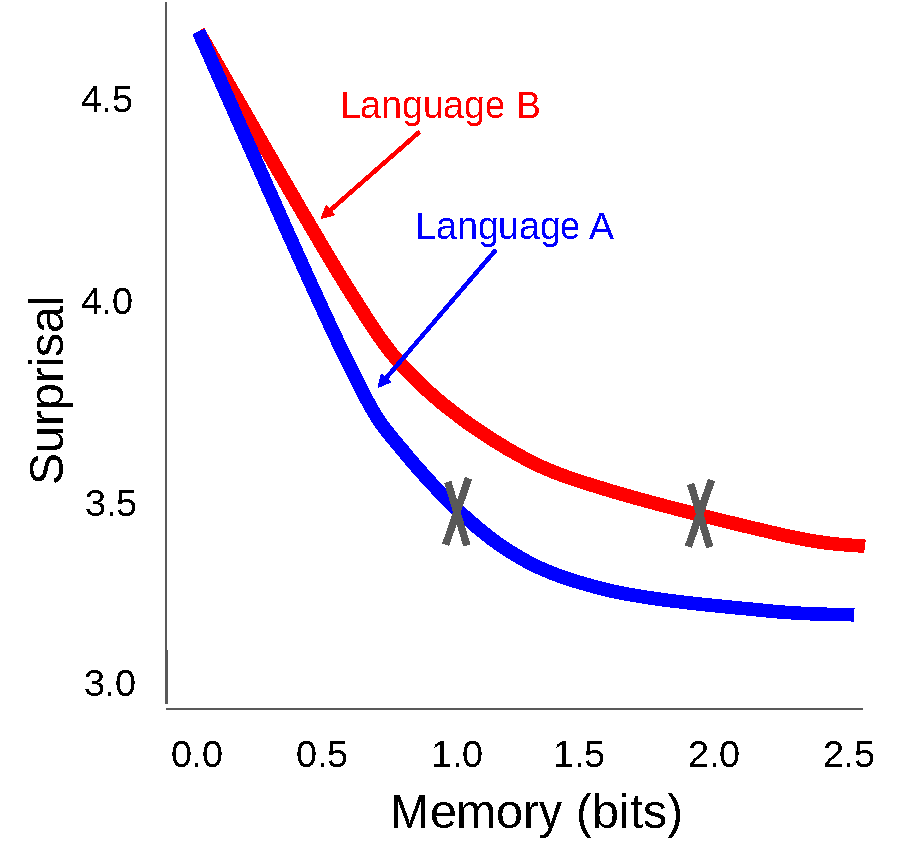
\includegraphics[width=0.5\textwidth]{figures-gdrive/tradeoff-schematic.pdf}
\caption{Example memory--surprisal tradeoff curves for two languages, $A$ and $B$. Achieving an average surprisal of 3.5 bits requires storing at least 1.0 bits in language $A$, while it requires storing 2.0 bits in language $B$. Language $B$ has a steeper memory--surprisal tradeoff than Language $A$, and requires less memory resources to achieve the same level of processing difficulty.}
\label{fig:examples}
\end{figure}

\subsection{Main hypothesis}

Having conceptually introduced the memory--surprisal tradeoff, we can state the main hypothesis of this work, the Efficient Tradeoff Curve Hypothesis.

\begin{adjustwidth}{6em}{6em}
\textbf{Efficient Tradeoff Curve Hypothesis:}\\
The order of elements in natural language is characterized by a distinctively steeper memory--surprisal tradeoff curve, compared to other possible orders.
\end{adjustwidth}
A steep tradeoff curve corresponds to memory efficiency, in the sense that it is possible to achieve a low level of processing difficulty (average surprisal $S_M$) while storing a relatively small amount of information about previous words (entropy of memory $H_M$).
We hypothesize that this property is reflected in grammatical structure and usage preferences across languages.


\subsection{Formal definition of the memory--surprisal tradeoff}
\label{sec:formal-tradeoff}

Here we provide the technical definition of the memory--surprisal tradeoff curve. % and relate it to concepts from information theory, rate--distortion theory, and statistical complexity theory.
Let $W$ be a stochastic process %\footnote{We will use $W$ to represent languages, and we will construct $W$ to be stationary. Large natural language texts are likely neither stationary nor ergodic \citep{debowski}. However, we are interested in explaining grammatical properties of languages, which mostly involve constraints among words within sentences, not within large texts as a whole. Therefore, we will represent a language using a stochastic process consisting of repeated independent samples from a distribution over sentences. This stochastic process is both stationary and ergodic.}
generating a stream of symbols extending indefinitely into the past and future: $\dots, w_{-2}, w_{-1}, w_0, w_{1}, w_{2}, \dots$. %indexed as $w_1, \dots, w_t, \dots$.
These symbols can represent words, morphemes, or other units for decomposing sentences into a sequence of symbols. 
We model this process as \emph{stationary} \citep{doob1953stochastic}, that is, the joint probability distributions of symbols at different time points depend only on their relative positions in time, not their absolute positions (see SI Section 1.1.1 for more on this modeling assumption).

Let $M$ be a memory encoding function.
We consider memory and surprisal costs at an arbitrary time point $t$.
%The process $W$ extends indefinitely into the past and future from this time point: $\dots, w_{t-2}, w_{t-1}, w_t, w_{t+1}, w_{t+2}, \dots$.
Recall that the surprisal for a specific word $w_t$ after a past word sequence $\dots, w_{t-2}, w_{t-1}$ encoded into a memory state $m_t$ is:
\begin{equation}
    -\log P(w_t | m_t).
\end{equation}
The \key{average surprisal} of the process $W$ under the memory encoding function $M$ is obtained by averaging over all possible past sequences $\dots, w_{t-2}, w_{t-1}$ with associated memory states $m_t$:
\begin{equation}
   S_M \equiv \sum_{w_t,m_t}  P(m_t) P(w_t|m_t) \left( -\log P(w_t | m_t) \right).
\end{equation}
where $w_t$ ranges over possible symbols, $m_t$ ranges over possible outputs of the memory encoding function $M$.
This quantity is known as the conditional entropy of $w_t$ given $m_t$ \citep[][p. 17]{cover2006elements}:
\begin{equation}
    S_M = H[w_t | m_t].
%    S_M \equiv \lim_{T\rightarrow\infty} \frac{1}{T} \sum_{t=1}^T \operatorname{H}[w_t | m_t],
\end{equation}
%where the notation $\operatorname{H}[\cdot | \cdot]$ indicates conditional entropy \citep[][p. 17]{cover2006elements}:
%\begin{equation}
%    \operatorname{H}[w_t|m_t] \equiv -\sum_{w_t,m_t} P(m_t) P(w_t|m_t) \log P(w_t|m_t).
%\end{equation}
Because the process $W$ is stationary, the average surprisal $S_M$ is independent of the choice of $t$ (see SI Section 1.1.2).
The lowest possible average surprisal for $W$ is attained when $m_t$ perfectly encodes all previous observed words.
This quantity is called the \key{entropy rate} of $W$ \citep[][pp. 74--75]{cover2006elements}:
\begin{equation}
    \label{eq:entropy-rate}
       S_\infty \equiv H[w_t | \dots, w_{t-2}, w_{t-1}],
%    S_\infty \equiv \lim_{t \rightarrow \infty} \frac{1}{T} \sum_{t=1}^T H[w_t | w_1, \dots, w_{t-1}].
\end{equation}
which again is independent of $t$ because $W$ is stationary.
We use the notation $S_\infty$ to suggest this idea of unlimited resources.
 The entropy rate of a stochastic process is the irreducible unpredictability of the process: the extent to which a stream of symbols remains unpredictable even for a predictor with unlimited resources. 
 The entropy rate $S_\infty$ of natural language text has been studied by \citet{shannon1951entropy}, \citet{bentz2017entropy}, and \citet{takahashi2018cross}. 
 Because the memory state $m_t$ is a function of the previous words $ \dots, w_{t-2}, w_{t-1}$, we can prove by the Data Processing Inequality \citep[][pp. 34--35]{cover2006elements} that the entropy rate must be less than or equal to the average surprisal for any memory encoding function $M$:
\begin{equation}
    \label{eq:entropy-rate-dpi}
    S_\infty \le S_M.
\end{equation}
If the memory state $m_t$ stores all information about the previous words $ \dots, w_{t-2}, w_{t-1}$, then we have $S_M = S_\infty$.
%Based on Eq.~\ref{eq:entropy-rate-dpi}, we can write the average surprisal $S_M$ as a sum of two non-negative terms,
%\begin{equation}
%    S_M = S_\infty + d_M,
%\end{equation}
%where $d_M$ is \key{memory distortion}: the extra surprisal incurred in addition to the unavoidable surprisal $S_\infty$, owing to the lossiness of the memory encoding function $M$. 
%The memory distortion $d_M$ is formally a Kullback-Leibler (KL) divergence:
%\begin{equation}
%    \label{eq:memory-distortion}
%    d_M = \lim_{t \rightarrow \infty} D_{\text{KL}} [ p(w_t | w_1, \dots, w_{t-1}) || p(w_t | m_t)].
%\end{equation}
%Finding a memory encoding function $M$ to minimize $S_M$ is equivalent to minimizing the memory distortion $d_M$.
%\mhahn{do we need to introduce the distortion $d_M$?}

Having defined average surprisal, we now turn to the question of how to define memory capacity. The average amount of information stored in the memory states $m_t$ is the average number of bits required to encode $m_t$. 
This is given by the entropy of the distribution over memory states, $H_M$: %, again averaged over all time points:
\begin{align}
    \label{eq:memory-entropy}
        H_M &\equiv \operatorname{H}[m_t] 
    %H_M &\equiv \lim_{T\rightarrow\infty} \frac{1}{T} \sum_{t=1}^T H[m_t] \\
\end{align}
where
\begin{equation}
    \operatorname{H}[m_t] = - \sum_m p(m_t = m) \log p(m_t=m)
\end{equation}
where $m$ runs over all possible states of the memory encoding $m_t$.
Again, because $W$ is stationary, this quantity does not depend on the choice of $t$ (see SI Section 1.1.2).


We will be imposing bounds on $H_M$ and studying the resulting values of $S_M$. 

\begin{definition}
The \key{memory--surprisal tradeoff curve} for a process $W$ is the lowest achievable average surprisal $S_M$ for each value of $H_M$. Let $R$ denote an upper bound on the memory entropy $H_M$; then the memory--surprisal tradeoff curve as a function of $R$ is given by
\begin{equation}
    \label{eq:ms-formal}
    D(R) \equiv \min_{M : H_M \le R} S_M,
\end{equation}
where the minimization is over all memory encoding functions $M$ whose entropy $H_M$ is less than or equal to $R$.
\end{definition}

The memory state $m_t$ is generally a lossy representation of the true context of words $w_1, \dots, w_{t-1}$, meaning that $m_t$ does not contain all the possible information about $w_1, \dots, w_{t-1}$. The mathematical theory of lossy representations is \key{rate--distortion theory} \citep[for an overview and key results, see][pp. 301--347]{cover2006elements}; this theory has seen recent successful application in cognitive science and linguistics as a model of rational action under resource constraints \citep{brady2009compression,sims2012ideal,sims2018efficient,zaslavsky2018efficient,schach2018quantifying,zenon2019information,gershman2020origin}. 
Rate--distortion theory studies curves of the form of Eq.~\ref{eq:ms-formal}, which quantify tradeoffs between negative utility (`distortion') and information (`rate'). %Our memory--surprisal tradeoff curve is a distortion--rate curve, with $H_M$ as the rate and $S_M$ as the distortion. It differs from the typical curve studied in rate--distortion theory in that we define rate using entropy, rather than mutual information \citep[see][for a discussion of some of the consequences of this formulation]{strouse-deterministic-2017}. 
%Our theoretical results still hold if we were to define rate using mutual information (see SI Section \REF).


\begin{figure}
	(a)
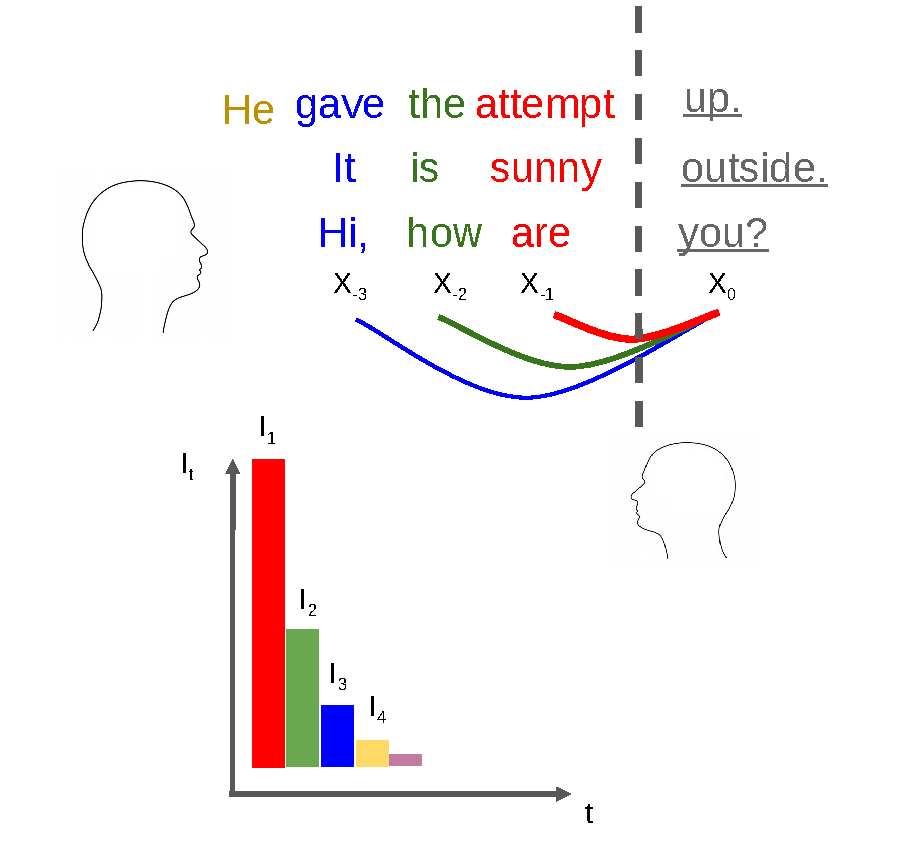
\includegraphics[width=0.4\textwidth]{figures-gdrive/mi-distance.pdf}
	(b)
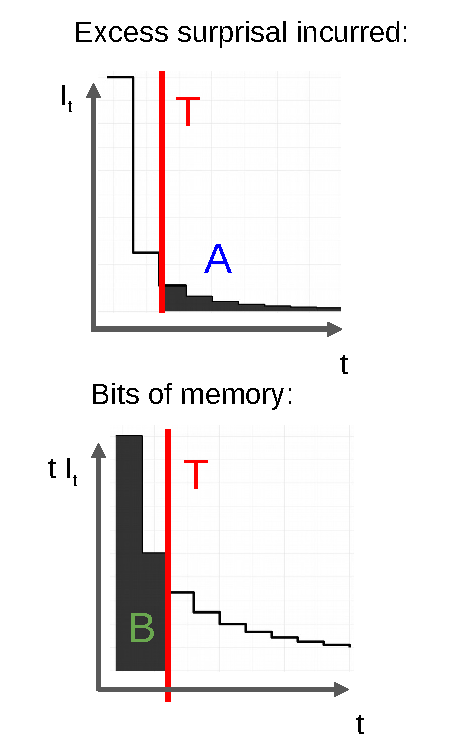
\includegraphics[width=0.25\textwidth]{figures-gdrive/theorem.pdf}
	\caption{
		(a) Conditional mutual information $I_t$ captures how much predictive information about the next word is provided, on average, by the word $t$ steps in the past.
		(b) Here we illustrate our theoretical result. We plot $I_t$ (top) and $tI_t$ (bottom) as functions of $t$. For any choice of $T$, a listener using $B$ bits memory (bottom) to represent prior observations will incur at least $A$ bits of extra surprisal beyond the entropy rate (top). 
}\label{fig:theorem}
\end{figure}

\subsection{Information locality}
\label{sec:infoloc}\label{sec:tradeoff}

The shape of the memory--surprisal tradeoff is determined in part by the grammatical structure of a language.
Some languages enable more efficient tradeoffs than others by forcing a listener to store more bits in memory to achieve the same level of average surprisal.

Here, we will demonstrate that the memory--surprisal tradeoff is optimized by languages with word orders exhibiting a property called \key{information locality}. Information locality means that words that depend on each other statistically are located close to each other in time. We will argue that information locality generalizes the well-known word order principle of dependency locality.

We will make our argument by defining a lower bound on the memory--surprisal tradeoff curve (Eq.~\ref{eq:ms-formal}). This lower bound represents an unavoidable cost associated with a certain level of memory usage $H_M$; the true average surprisal $S_M$ might be higher than this bound. 

Our argument will make use of a quantity called \key{mutual information}. Mutual information is the most general measure of statistical association between two random variables. The mutual information between two random variables $X$ and $Y$, conditional on a third random variable $Z$, is defined as:
\begin{align}
\label{eq:mi}
    I[X:Y|Z] &\equiv \sum_{x,y,z} P(x,y,z) \log \frac{P(x,y|z)}{P(x|z)P(y|z)} \text{ bits} \\
    \nonumber
    &= H[X|Z] - H[X|Y,Z] \\
    \nonumber
    &= H[Y|Z] - H[Y|X,Z].
\end{align}
Mutual information is always non-negative. It is zero when $X$ and $Y$ are conditionally independent given $Z$, and positive whenever $X$ gives any information that makes the value of $Y$ more predictable, or vice versa. 

We will study the mutual information structure of natural language sentences, and in particular the mutual information between words at certain distances in linear order. We define the notation $I_t$ to mean the mutual information between words at distance $t$ from each other, conditional on the intervening words:
\begin{align}
    \nonumber
    I_t &\equiv I[w_t : w_0 | w_1, \dots, w_{t-1}] \\
    \nonumber
    &= H[w_t | w_1, \dots, w_{t-1}] - H[w_t | w_0, \dots, w_{t-1}].
\end{align}
This quantity, visualized in Figure~\ref{fig:theorem}(a), measures how much predictive information is provided about the current word by the word $t$ steps in the past.
It is a statistical property of the language, and can be estimated from large-scale text data.

Equipped with this notion of mutual information at a distance, we can now state our theorem:
\begin{thm}\label{prop:suboptimal}(Information locality bound)
For any positive integer $T$, let $M$ be a memory encoding function such that
\begin{equation}
\label{eq:memory-bound}
H_M \le \sum_{t=1}^T t I_t.    
\end{equation}
Then we have a lower bound on the average surprisal under the memory encoding function $M$:
\begin{equation}
\label{eq:surprisal-bound}
S_M \ge S_\infty + \sum_{t=T+1}^\infty I_t.
\end{equation}
\end{thm}
A formal proof based on the Comprehension Postulates 1--3 is given in Appendix Section 1.2.

\paragraph{Interpretation} The theorem means that a predictor with limited memory capacity will always be affected by surprisal cost arising from long-term statistical dependencies of length greater than $T$, for some finite $T$. This is why we call the result `information locality': processes are easier to predict when most statistical dependencies are short-term (shorter than $T$). Below we explain in more detail how this interpretation matches the mathematics of the theorem.

The quantities in the theorem are illustrated visually in Figure~\ref{fig:theorem}. Eq.~\ref{eq:memory-bound} describes a memory encoding function which has enough capacity to remember the relevant information from at most $T$ words in the immediate past. The minimal amount of memory capacity which would be required to retain this information is the sum $\sum_{t=1}^T t I_t$, reflecting the cost of holding $I_t$ bits in memory for $t$ timesteps up to $t=T$. 

The information locality bound theorem says that the surprisal cost for this memory encoding function is at least $S_\infty + \sum_{t=T+1}^\infty I_t$ (Eq.~\ref{eq:surprisal-bound}). The first term $S_\infty$ is the entropy rate of the process, representing the bits of information in the process which could not have been predicted given any amount of memory. The second term $\sum_{t=T+1}^\infty I_t$ is the sum of all the relevant information contained in words \emph{more} than $T$ timesteps in the past (see Figure~\ref{fig:theorem}(b)). These correspond to bits of information in the process which \emph{could have} been predicted given infinite memory resources, but which were not, due to the limit on memory usage.

The theorem gives a lower bound on the memory--surprisal tradeoff curve, meaning that there is no memory encoding function $M$ with capacity $H_M$ which achieves lower average surprisal than Eq.~\ref{eq:surprisal-bound}. In terms of psycholinguistics, if memory usage is bounded by Eq.~\ref{eq:memory-bound}, then processing cost of at least Eq.~\ref{eq:surprisal-bound} is inevitable.
Importantly, the bound holds for \emph{any} memory encoding function $M$, including functions that do not specifically keep track of a window of the past $T$ words.

\begin{figure*}
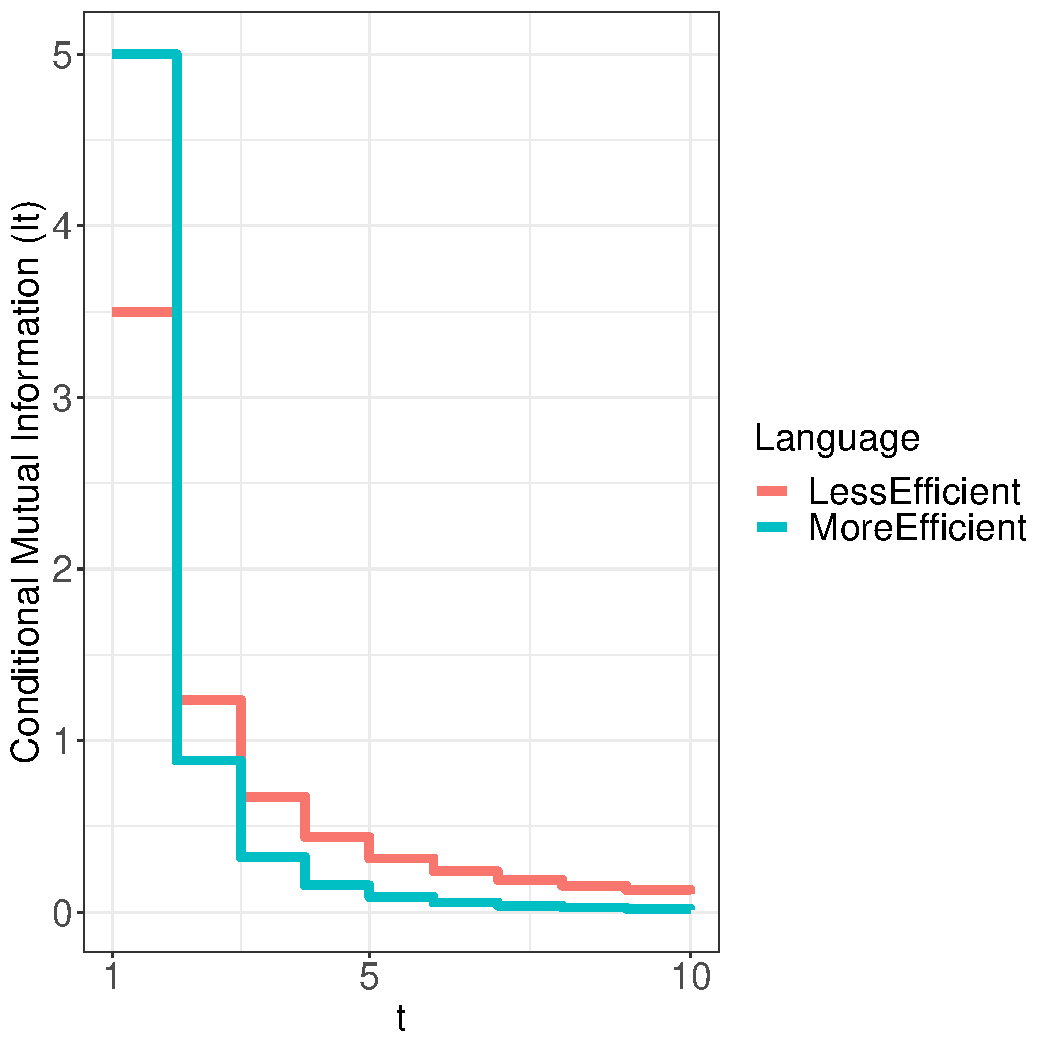
\includegraphics[width=0.45\textwidth]{figures/decay.pdf}
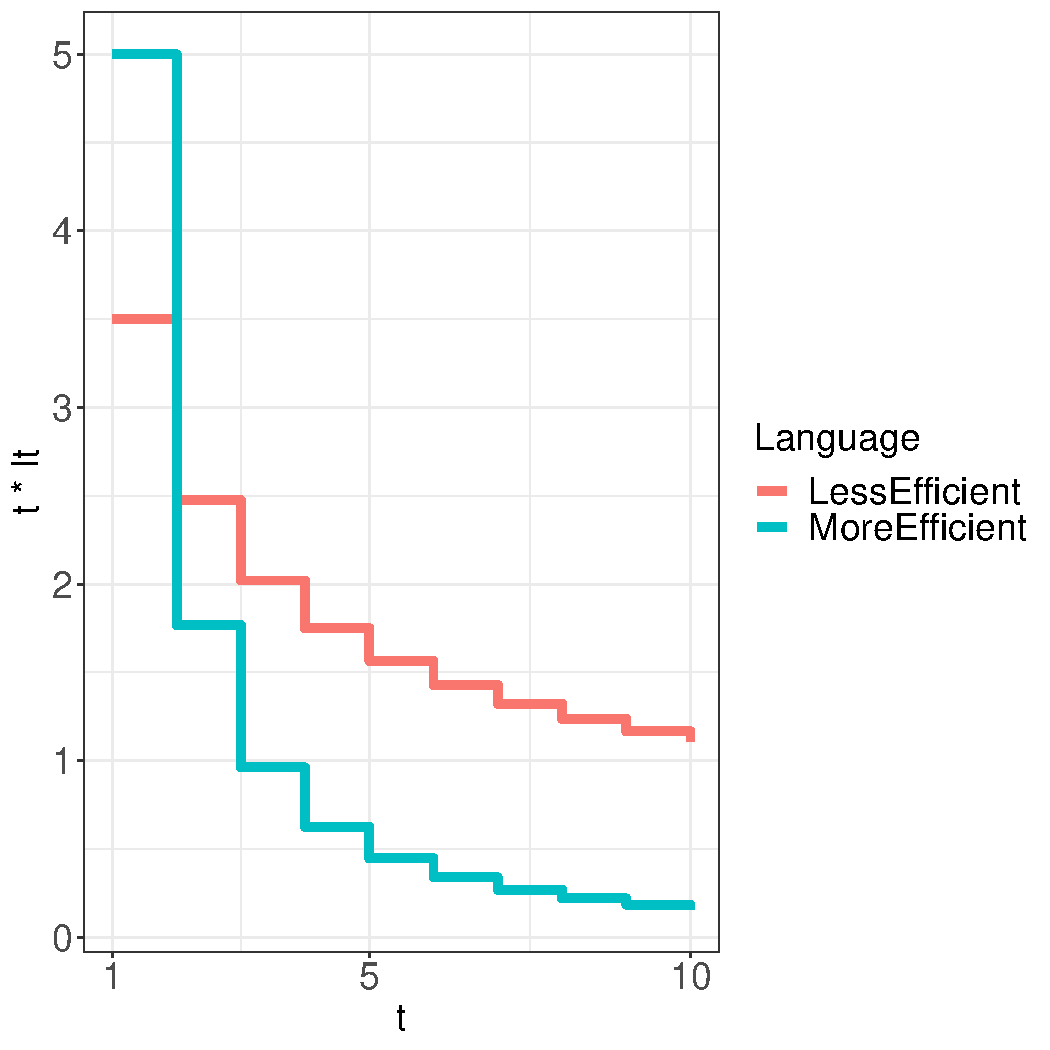
\includegraphics[width=0.45\textwidth]{figures/memory.pdf}
%
	\caption{Left: $I_t$ as a function of $t$, for two different hypothetical languages. $I_t$ decays faster for the MoreEfficient language: Predictive information about the present observation is concentrated more strongly in the recent past. Right: $t \cdot I_t$ as a function of $t$ for the same languages. }\label{fig:basic}
\end{figure*}

\begin{figure}
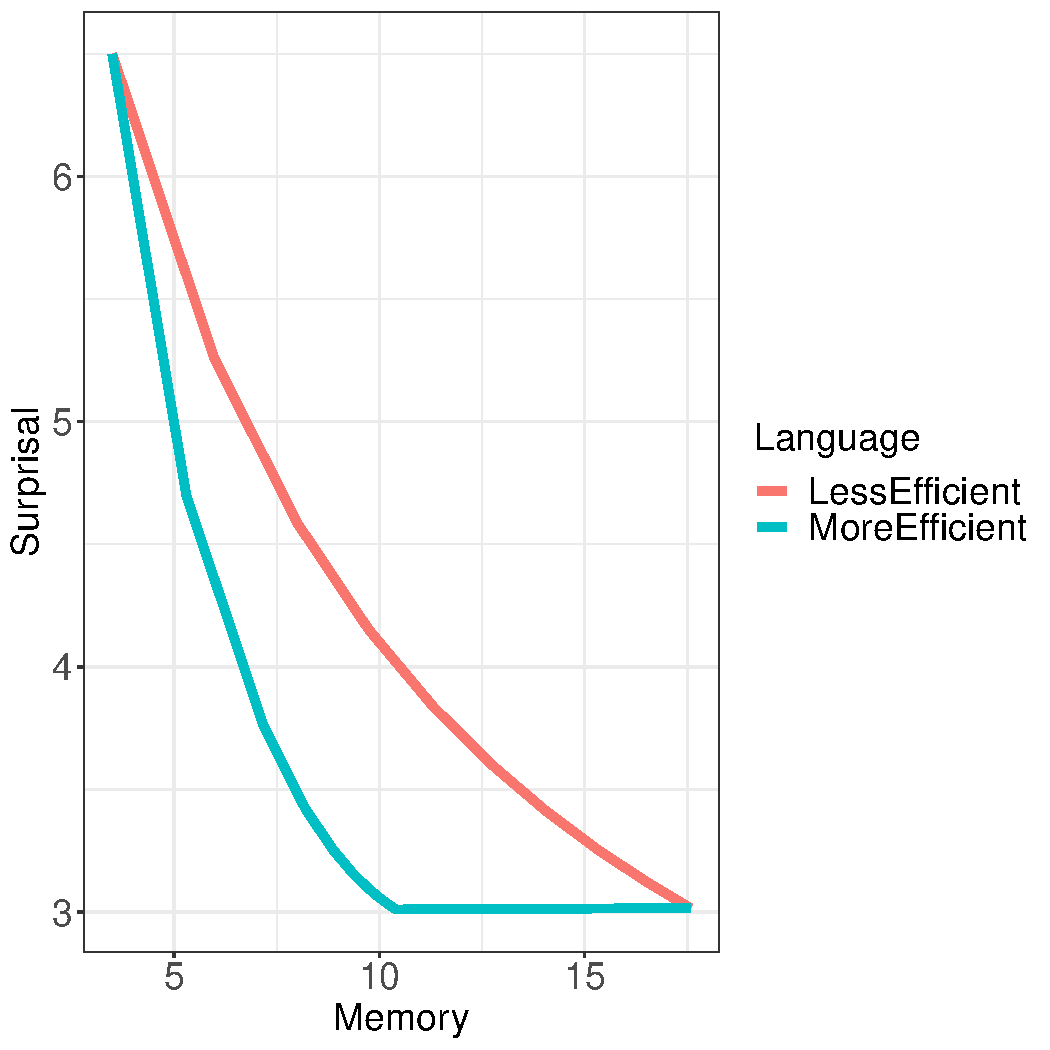
\includegraphics[width=0.45\textwidth]{figures/listener-tradeoff.pdf}
	\caption{Listener's memory-surprisal tradeoff for the two hypothetical languages in Figure~\ref{fig:basic}. Recall that the MoreEfficient language has a faster decay of conditional mutual information $I_t$. Correspondingly, this figure shows that a listener can achieve lower average surprisal at the same level of memory load.}\label{fig:listener-tradeoff}
\end{figure}

Eq.~\ref{eq:memory-bound} means that maintaining long-term dependencies requires higher memory usage. Carrying the same amount of information over longer distances requires more memory; this fact is reflected in the factor $t$ inside each term of the sum. 
The result is that modeling long-term statistical dependencies is more costly in terms of memory usage than modeling shorter ones; this cost can manifest in memory storage or in surprisal.
The information locality bound theorem demonstrates in a highly general way that language comprehension requires less memory resources when statistical dependencies are mostly short-term. 

Because processing long-term dependencies requires higher memory usage, the theorem also implies that a language will be easier to process when most of the predictive information about a word is concentrated close to that word in time---that is, when $I_t$ falls off rapidly as $t \rightarrow \infty$. When memory capacity is limited, then there must be some timescale $T$ such that a listener appears to be affected by excess surprisal arising from statistical dependencies of length greater than $T$. A language avoids such cost to the extent that it avoids dependencies with a time-span larger than $T$.

We illustrate the theorem in Figure~\ref{fig:basic}.
We consider two hypothetical languages, LessEfficient and MoreEfficient, where $I_t := 5t^{-1.5}$ for LessEfficient and $I_t := 3.5 t^{-2.5}$ for MoreEfficient.
The curves of $I_t$, as a function of the distance $t$, are shown in Figure~\ref{fig:basic} (left).
In both cases, $I_t$ converges to zero as $t$ grows to infinity. 
However, $I_t$ decays more quickly for language MoreEfficient.
This means that predictive information about an observation is concentrated more strongly in the recent past.
In Figure~\ref{fig:basic} (right), we show $t\cdot I_t$ as a function of $t$.
Note that the area under the curve is equal to (\ref{eq:memory-bound}).
This area is smaller for the MoreEfficient language, as $I_t$ decays more quickly there.  
In Figure~\ref{fig:listener-tradeoff}, we show the resulting bounds on memory-surprisal tradeoffs of the two languages.  
As $I_t$ decays faster for language MoreEfficient, it has a more efficient memory-surprisal tradeoff, allowing a listener to achieve strictly lower surprisal across a range of memory values.





\section{Study 1: Memory and Dependency Length}\label{sec:toy-study}

So far, we have proven that there must exist a trade-off between memory and surprisal, and that this trade-off is optimized when languages have relatively short-term dependencies. Here, we illustrate the linguistic predictions of our theoretical results, and confirm that favored word orders with short syntactic dependencies do indeed optimize the memory--surprisal tradeoff in a toy language.

We will illustrate the operation of our theoretical framework by reanalyzing the data from \cite{fedzechkina-human-2017}.
This is a miniature artificial language study that showed a bias for dependency locality in production in artificial language learning. 
We will show that the languages which were favored in the artificial language learning experiment are those which optimize the memory--surprisal trade-off.

\subsection{Background: \citet{fedzechkina-human-2017}}

\citet{fedzechkina-human-2017} conducted a miniature artificial language learning experiment in which participants were exposed to videos describing simple events, paired with sentences in an articial language of the form Subject--Object--Verb or Object--Subject--Verb, in equal proportion, with free variation between these two word orders. The subject and the object were either simple nouns, or complex noun phrases with modifiers. Participants were trained to produce sentences in response to videos.

Crucially, \citet{fedzechkina-human-2017} set up the experiment such that in all training trials, other the subject and the object were both simple, or they were both complex. Then, after participants were sufficiently skilled in the use of the artificial language, they were asked to produce sentences describing videos with mixed complexity of noun phrases. The possible word orders that could be produced in this mixed-complexity setting are shown in Figure~\ref{tab:artificial}; the orders marked $A$ would create short dependencies, and the orders marked $B$ would create long dependencies. 
\begin{figure}
	\textbf{A Orders: Short Dependencies}

	OSV: [[Adjective Noun Postposition] Noun-\textsc{Case}] Noun Verb

	SOV: [[Adjective Noun Postposition] Noun] Noun-\textsc{Case} Verb

%
%	OSV:
%		\begin{tabular}{ccc}
%%			Object & Subject & Verb \\
%			\fbox{\begin{tabular}{llllll}
%				\fbox{\begin{tabular}{llll} Adjective &Noun &Postposition\end{tabular}} & Noun-\textsc{\textsc{Case}}
%					\end{tabular}} & \fbox{\begin{tabular}{l}Noun\end{tabular}} & \fbox{\begin{tabular}{l}Verb\end{tabular}}  \\
%		\end{tabular}
%\\
%
%SOV:
%		\begin{tabular}{ccc}
%			%			Subject & Object & Verb \\
%			\fbox{\begin{tabular}{llllll}
%				\fbox{\begin{tabular}{llll} Adjective &Noun &Postposition\end{tabular}} & Noun
%					\end{tabular}} & \fbox{\begin{tabular}{l}Noun-\textsc{\textsc{Case}}\end{tabular}} & Verb \\
%		\end{tabular}
%\\
%\\

	\textbf{B Orders: Long Dependencies}

	SOV: Noun [[Adjective Noun Postposition] Noun-\textsc{Case}] Verb

	OSV: Noun-\textsc{Case} [[Adjective Noun Postposition] Noun] Verb
%
%		\begin{tabular}{ccc}
%%			Subject & Object & Verb \\
%			 \fbox{\begin{tabular}{l}Noun\end{tabular}} &  \fbox{\begin{tabular}{llllll}
%				\fbox{\begin{tabular}{llll} Adjective &Noun &Postposition\end{tabular}} & Noun-Case
%		\end{tabular}}  &  \fbox{\begin{tabular}{l}Verb\end{tabular}}  \\
%		\end{tabular}
%\\
%		\begin{tabular}{ccc}
%%			Object & Subject & Verb \\
%			\fbox{\begin{tabular}{l}Noun-Case\end{tabular}} & \fbox{\begin{tabular}{llllll}
%				\fbox{\begin{tabular}{llll} Adjective &Noun &Postposition\end{tabular}} & Noun
%		\end{tabular}} & Verb \\
%		\end{tabular}
%
			\caption{Production targets in the miniature artificial language from \cite{fedzechkina-human-2017}. The language has head-final order, with free variation between SO and OS orders. When one of the arguments is much longer than the other, placing the longer one first ($A$ orders) shortens syntactic dependencies, compared to $B$ orders.}\label{tab:artificial}

\end{figure}

\citet{fedzechkina-human-2017} hypothesized, and indeed found, that participants favored the $A$ orders over the $B$ orders, despite the fact that there was no pattern in the participants' training input which would have favored $A$ over $B$. That is, when exposed to input which was ambiguous with respect to language $A$ or $B$, participants favored language $A$. \citet{fedzechkina-human-2017} explain the result in terms of dependency locality, because the $A$ orders create short dependencies between the verb and its arguments, and the $B$ orders create long dependencies.

\subsection{Calculating the memory--surprisal trade-off for the artificial languages}

We hypothesize, in line with our Main Hypothesis, that the favored language $A$ has a steeper memory--surprisal trade-off curve than the disfavored language $B$. Because of the controlled nature of this artificial language, we are able to test this hypothesis by exactly computing the bound on memory as given in Theorem~\ref{prop:suboptimal}. In fact, for this toy process, we can prove that the bound provided by the theorem is achievable, meaning that our computations reflect the true memory--surprisal trade-off curve, and not only a lower bound on it.

We only consider the head-final version of \citet{fedzechkina-human-2017}'s artificial language. This is because our bound on the memory--surprisal trade-off curve is invariant under reversal of a language. That is, if we take a language and reverse the order of all the words in all its sentences, we would measure the same lower bound on the memory--surprisal trade-off curve (for a proof, see SI Section \REF). Therefore, strictly head-final and strictly head-initial languages are equivalent under our bound.\footnote{Note that this invariance to reversal applies only to our \emph{lower bound} on the memory-surprisal trade-off curve; the true curve is not generally invariant to word order reversal \citep{crutchfield-times-2009}.} 

%The language has consistent head-final order, and uses case marking on objects.
%The relevant production targets are transitive sentences where one of the two arguments is much longer than the other, due to the presence of a PP modifier, as shown in Table~\ref{tab:artificial}.
%The language has variable order of subjects and objects; for the production targets, the B versions produce much longer dependencies than the A versions.
%Dependency Length Minimization thus predicts that speakers are more likely to use the A versions.
%\cite{fedzechkina-human-2017} confirmed this experimentally.

We constructed a stochastic process representing the language consisting of sentences with the $A$ orders from Figure~\ref{tab:artificial}, and one language consisting of the $B$ orders. Following the experimental setup of \cite{fedzechkina-human-2017}, we assigned equal probability to the two possible configurations per language, and used a separate set of nouns (inanimate nouns) for the embedded noun in the long phrase.

% TODO: Does the process only include those orders, or does it also include the SOV and OSV orders with equal-complexity O and S?

We interpreted each of the two languages as a stationary processes, extending infinitely in both directions, by concatenating independent samples drawn from the language.
We computed (\ref{eq:memory-bound}) from a chain of 1000 independently sampled sentences, for each of the two versions of the toy language.
% TODO: More on how this was done.			
% TODO: Convert nats to bits

\subsection{Results}	

\begin{figure*}
\centering
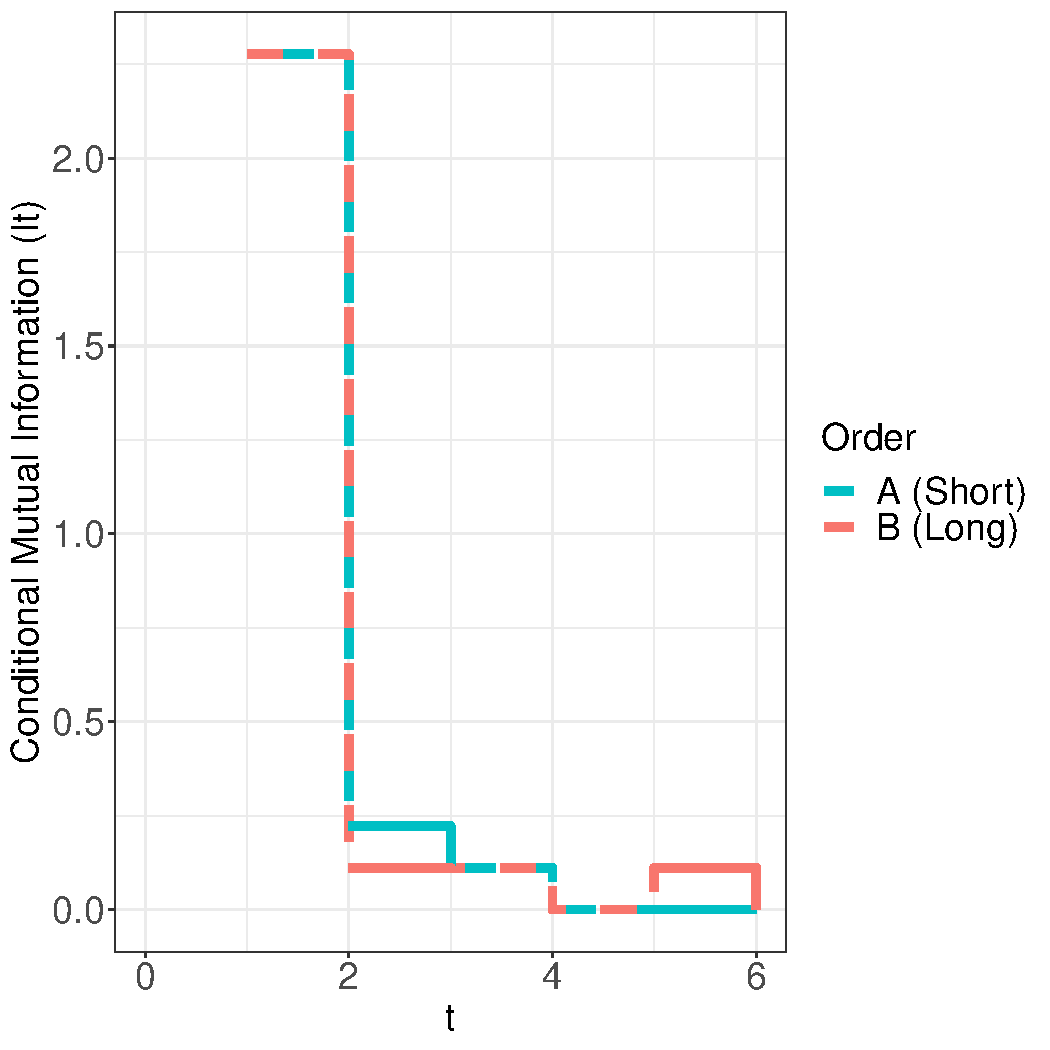
\includegraphics[width=0.45\textwidth]{figures/toy-mis.pdf}
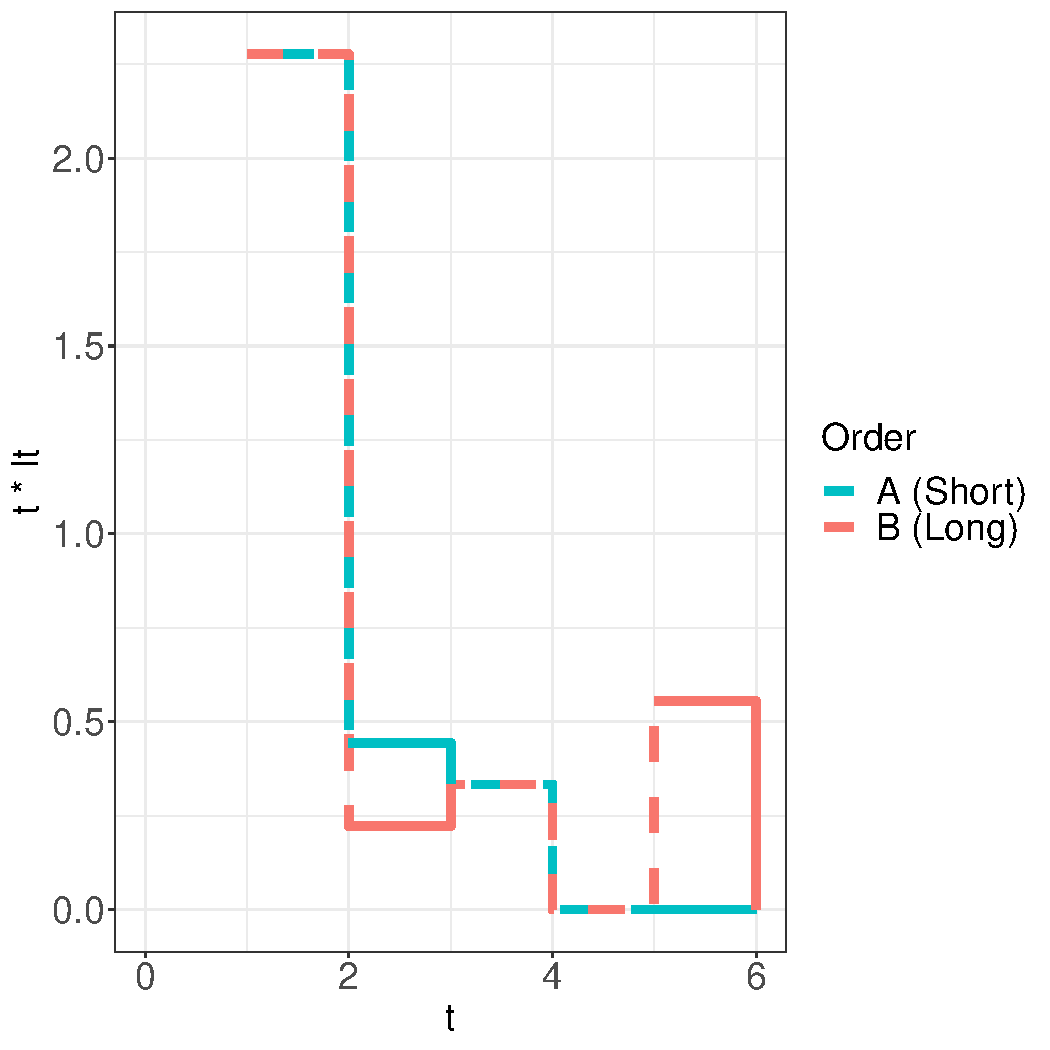
\includegraphics[width=0.45\textwidth]{figures/toy-t-mis.pdf}
%
	\caption{Left: Decay of conditional mutual information $I_t$, as a function of the distance $t$, for the two versions in the artificial language. The areas under the two curves are identical, corresponding to the fact that both orders are equally predictable. However, mutual information decays faster in language $A$.\ \ \ Right: The minimal memory requirement $t I_t$ to store $I_t$ bits of information for timespan $t$, as a function of $t$. The area under the $B$ curve is larger, corresponding to larger memory demand for this order.}\label{fig:toy-mis}
\end{figure*}

Figure~\ref{fig:toy-mis} (left) shows the curve of the conditional mutual information $I_t$ as a function of the distance $t$, for the two languages $A$ and $B$. 
The curves differ at $t=2$ and $t=5$: 
About 0.073 units of predictive information that are at distance $t=2$ in the $A$ orders are moved to $t=5$ in the $B$ orders.
The source of the difference lies in predicting the presence and absence of a case marker on the second argument---i.e., whether to anticipate a subject or object.
In the $A$ orders, considering the last two words is sufficient to make this decision.
In the $B$ orders, it is necessary to consider the word before the long second constituent, which is five words in the past.

The total amounts of predictive information---corresponding to the area under the $I_t$ curve----are the same for both languages, indicating that both languages are equally predictable.
			
However, we will see that the memory demands are different.
Figure~\ref{fig:toy-mis} (right) shows the minimal memory requirements for remembering predictive information at a distance $t$ ($t\cdot I_t$) as a function of $t$.
As $I_t$ decays faster in $A$ orders, the total area under the curve now differs between $A$ and $B$, and is larger in $B$.
			Therefore, achieving the same predictive accuracy in language $B$ requires more memory resources than in language $A$.
			%This area corresponds to the lower bound in (\ref{eq:memory-bound}), and is 2.21 nats in A orders, and 2.43 nats in B orders.

%While (\ref{eq:memory-bound}) is a general lower bound, it can be proven that this bound is actually tight in the case of this specific example.\footnote{This can be shown by computing the causal states and then showing that the crypticity is zero, both of which is tractable in the case of this small-scale artificial language.}
%That is, a speaker who optimally allocates memory resources will spend 2.21 nats in A orders, and 2.43 nats in B orders.

\begin{figure}
\centering
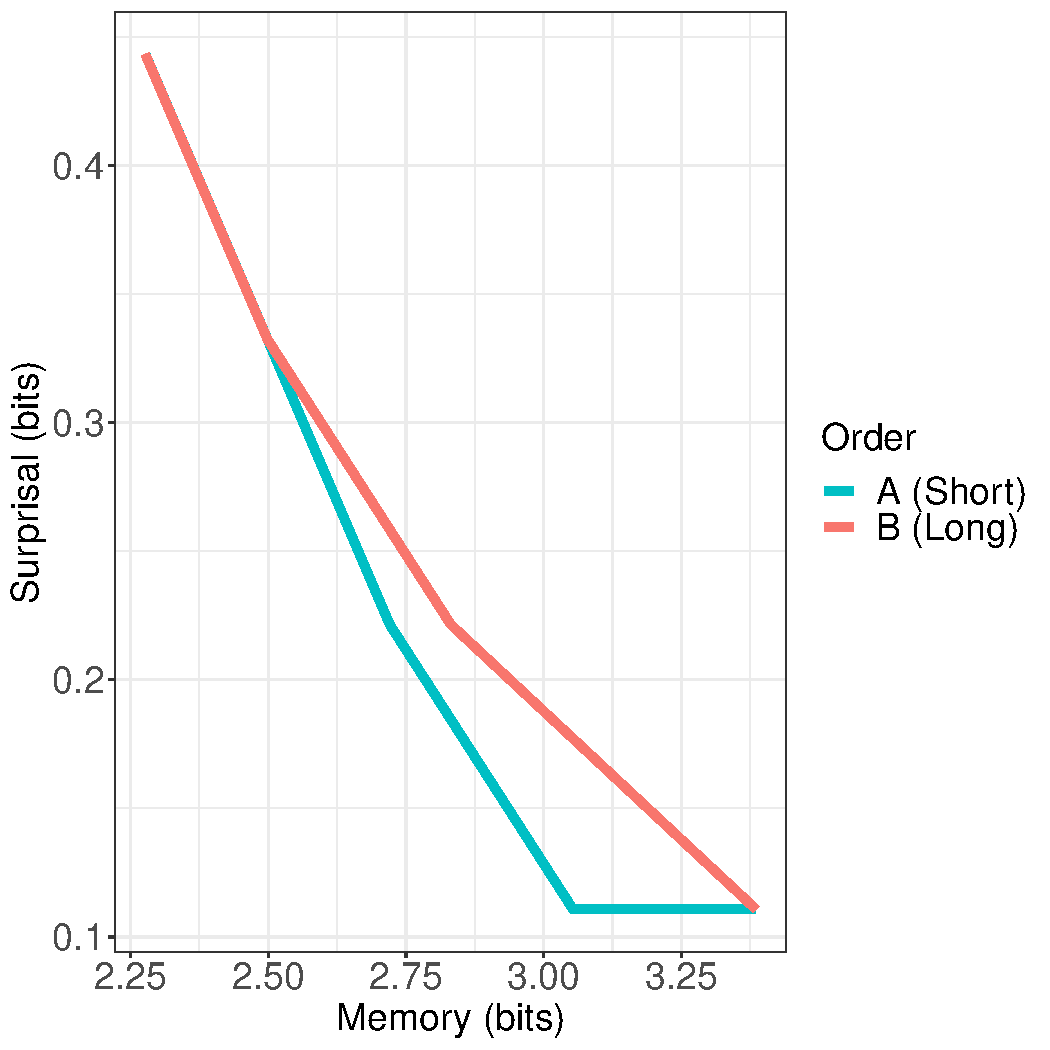
\includegraphics[width=0.45\textwidth]{figures/toy-mem-surp.pdf}
	\caption{Tradeoff between listener memory and surprisal, for the two versions of the artificial language from \cite{fedzechkina-human-2017}. Language $A$ requires less memory at the same level of surprisal. }
	\label{fig:toy-listener-tradeoff}
\end{figure}

In Figure~\ref{fig:toy-listener-tradeoff}, we show the resulting memory--surprisal trade-off curve for the two versions of the artificial language from \cite{fedzechkina-human-2017}, obtained by tracing our all values of $T=1, 2, \dots$ in the theorem, and connecting the points linearly.\footnote{Linear interpolation is justified because rate-distortion curves such as the memory-surprisal tradeoff curve are convex \citep{berger2003rate}.}
The curve shows that, at any desired level of surprisal, language $A$ requires at most as much memory as language $B$.
For reaching optimal surprisal, the empirically-favored language $A$ requires strictly less memory.


%It is important to stress that, even though we computed this value by considering the number of words impacting predictions at a given point in time, this bound holds independently of the actual implementation and architecture of memory and predictions.





%Both languages have the same overall entropy rate, but they differ in the distribution of predictive information.
%
%plot of $I_t$
%
%The areas under the curves are identical.
%
%good version
%
%%CONTEXT LENGTH 0   2.06856758681  9997.93143241   0.0
%%CONTEXT LENGTH 1   0.29195106479  1.77661652202   1.77661652202
%%CONTEXT LENGTH 2   0.0729865489103  0.21896451588   2.21454555377
%%CONTEXT LENGTH 3   0.0729865489103  0.0   2.21454555377
%%CONTEXT LENGTH 4   0.0729865489103  0.0   2.21454555377
%%CONTEXT LENGTH 5   0.0729865489103  0.0   2.21454555377
%%CONTEXT LENGTH 6   0.0729865489103  0.0   2.21454555377
%
%bad version
%
%%CONTEXT LENGTH 0   2.06937301571  9997.93062698   0.0
%%CONTEXT LENGTH 1   0.291673373027  1.77769964269   1.77769964269
%%CONTEXT LENGTH 2   0.145830550934  0.145842822093   2.06938528687
%%CONTEXT LENGTH 3   0.145830550934  0.0   2.06938528687
%%CONTEXT LENGTH 4   0.145830550934  0.0   2.06938528687
%%CONTEXT LENGTH 5   0.0729152754672  0.0729152754672   2.43396166421
%%CONTEXT LENGTH 6   0.0729152754672  0.0   2.43396166421
%%CONTEXT LENGTH 7   0.0729152754672  0.0   2.43396166421
%%
%
%
%
%%
%%grammar:
%%
%%S $\rightarrow$ Obj Subj V (1/2) | Subj Obj V (1/2)
%%
%%Obj $\rightarrow$ NP di
%%
%%Subj $\rightarrow$ NP
%%
%%NP $\rightarrow$ N (3/4) | PP NP (1/8) | Adj NP (1/8)
%%
%%PP $\rightarrow$ NP P
%%
%
%




\subsection{Discussion}

In a reinterpretation of previous experimental findings, we showed that the languages which are favored in artificial language learning experiments are those which optimize the memory--surprisal trade-off. 
This is evidence that learners and/or speakers have a bias toward word orders that optimize the trade-off. 
Furthermore, this result solidifies the link between the memory--surprisal trade-off and more traditional notions from linguistics, such as dependency locality. 
We found that the word orders which are optimal from the perspective of dependency locality are also those orders which are optimal from the perspective of the memory--surprisal trade-off.




\section{Study 2: Large-Scale Evidence that Word Orders Optimize Memory-Surprisal Tradeoff}
\label{sec:main-experiment}

We now investigate whether word orders as found in natural language reflect optimization for the memory--surprisal trade-off more generally.
To this end, we compare the memory--surprisal trade-offs of 52 actual languages to those of counterfactual baseline languages, which differ from the actual languages only in their word order rules. This method of comparison against counterfactual baseline languages was introduced by \citet{gildea-optimizing-2007,gildea-grammars-2010} has been applied to study optimization-based models of word order universals by \citet{futrell-large-scale-2015}, \citet{gildea-human-2015}, and \citet{hahn2020optimization}.

Here, we describe how we measure the memory--surprisal trade-off in corpora, and how we generate counterfactual baseline languages. In Section~\ref{sec:main-experiment-results}, we compare the trade-off in real corpora against the trade-off in the counterfactual baselines.

\subsection{Measuring the memory--surprisal trade-off in corpora}

The key to evaluating the memory-surprisal tradeoff from corpus data is the set of quantities $I_t$, the  mutual information between words at distance $t$ conditional on the intervening words. 
All that is required is to estimate the quantities $I_t$; then these can be plugged in to Theorem~\ref{prop:suboptimal} to give a lower bound on the memory--surprisal trade-off. 

The quantities $I_t$ can be estimated as the difference between the average surprisal of Markov models that have access to the last $t-1$ or $t$ words.
That is, if we have a $t$th-order Markov model with average surprisal
\begin{equation*}
    S_t = H[w_t | w_0, \dots, w_{t-1}]
\end{equation*}
and a $(t-1)$th-order Markov model with average surprisal
\begin{equation*}
    S_{t-1} = H[w_t | w_1, \dots, w_{t-1}],
\end{equation*}
then we can calculate $I_t$ straightforwardly in the following way:
\begin{align}
    \nonumber
    I_t &= I[w_t : w_0 | w_1, \dots, w_{t-1}] \\
    \nonumber
    &= S_{t-1} - S_t.
\end{align}
Therefore, to evaluate $I_t$, all we need is a way of fitting Markov models of order $t$ and $t-1$. Then the average surprisal values can be extracted from these models straightforwardly.

To fit Markov models to the data, we use neural language models. In particular, we use Recurrent Neural Networks with Long Short-Term Memory architectures \citep{hochreiter-long-1997}. 
Neural network models are the basis of the state-of-the art in statistical modeling of language and in predicting the surprisal effect on reading times~\citep{frank-insensitivity-2011,goodkind-predictive-2018}.
See Supplementary Materials Section X for details on how these models were fit to data, and see Supplementary Materials Sections Y and Z for control studies using other methods of estimating $I_t$ (based on $n$-gram models and PCFG chart parsers). The results of these control studies are in agreement with the neural network results presented in this section.

In order to evaluate the values $S_t$, we calculated the average surprisal under the $t$th-order Markov model on held-out data, different from the data that was used to train the model. By evaluating on held-out data, we avoid underestimating the value of $S_t$ due to overfitting.

\subsection{Data}
We draw on corpora annotated with syntactic structures.
The Universal Dependencies project has compiled such annotated corpora for several dozen languages~\citep{nivre-universal-2017}.
These are annotated in the format of Dependency Grammar.

\paragraph{Dependency Grammar}
In dependency corpora, sentences are annotated with \emph{dependency trees} (Figure~\ref{fig:dependency}).
These are directed trees describing the grammatical relations among words. For example, the arcs labeled ``obj'' represent that the noun in question is the \emph{direct object} if the verb, rather than e.g. the subject or an indirect object.
A dependency arc is drawn from a \emph{head} (e.g. TODO in Figure TODO) to a \emph{dependent} (e.g. TODO).
Dependency trees can be defined in terms of many different syntactic theories \citep{corbett1993heads}.
Although there are some differences in how different formalisms would draw trees for certain sentences, there is broad enough agreement about dependency trees that it has been possible to develop large-scale dependency-annotated corpora of text from dozens of languages \citep{nivre2017universal}.

\begin{figure}
\centering
\begin{dependency}[theme = simple]
   \begin{deptext}[column sep=1em]
	   I \&	   wrote \& risāla \& li \& sadīq  \\
   \end{deptext}
	%   \deproot{3}{ROOT}
   \depedge{1}{2}{obj}
	%   \depedge[edge start x offset=-6pt]{2}{5}{ATT}
   \depedge{1}{4}{obl}
   \depedge{4}{3}{case}
   %\depedge[arc angle=50]{7}{6}{ATT}
\end{dependency}
	\caption{TODO Dependencies example}\label{fig:dependency}
\end{figure}

\paragraph{Selection of Languages}
We considered all languages for which there are Universal Dependencies 2.4 treebanks with a total of at least 500 sentences of training data.
We excluded data from historical languages.\footnote{Historical languages excluded: Ancient Greek, Classical Chinese, Coptic, Gothic, Latin, Old Church Slavonic, Old French.}
%While running this experiment, data from additional languages became available that also had enough data, through the Universal Dependencies 2.4 release. 
This resulted in 54 languages.

\paragraph{Processing of Corpora}
For each of these languages, we pooled all available corpora in one dataset.
We excluded corpora that primarily contain code-switched text\footnote{Hindi English corpus}, or text created by non-native speakers.\footnote{ESL for English, CFL for Chinese.}
Most Universal Dependencies corpora have a predefined split into \emph{training}, \emph{held-out} (also known as \emph{development}), and \emph{test} partitions.
%While larger corpora have all three partitions, smaller corpora often have only some of these partitions.
In most cases, we used the predefined data split, separately pooling data from the different partitions. 
For some languages with little data, there is no predefined training partition, or the training partition is smaller than the other partitions.
In these cases, we redefined the split to obtain more training data.
For these languages, we pooled all the available partitions, used 100 randomly selected sentences as held-out data, and used the remainder as training data.\footnote{This affects Amharic, Armenian, Breton, Buryat, Cantonese, Faroese, Kazakh, Kurmanji, Naija, Thai, and Uyghur.}
We did not make use of the \textit{test} partitions here.
We provide the sizes of the resulting datasets in Table~\ref{tab:corpora}.

\subsection{Defining baselines}

We construct counterfactual ordering grammars that define consistent ordering rules similar to those found in actual languages.
For instance, these grammars will specify which dependents precede or follow their heads (e.g., whether objects follow or precede verbs, whether adjectives follow or precede nouns), and the relative order of different dependents on the same side of the head (e.g., whether noun phrases have order adjective-numeral-noun or numeral-adjective-noun). Our formalism of ordering grammars adapts the method of \citet{gildea-optimizing-2007,gildea-grammars-2010,gildea-human-2015} to the setting of dependency corpora, following \citet{futrell-large-scale-2015} and \citet{hahn2020optimization}.


\begin{figure}
\centering
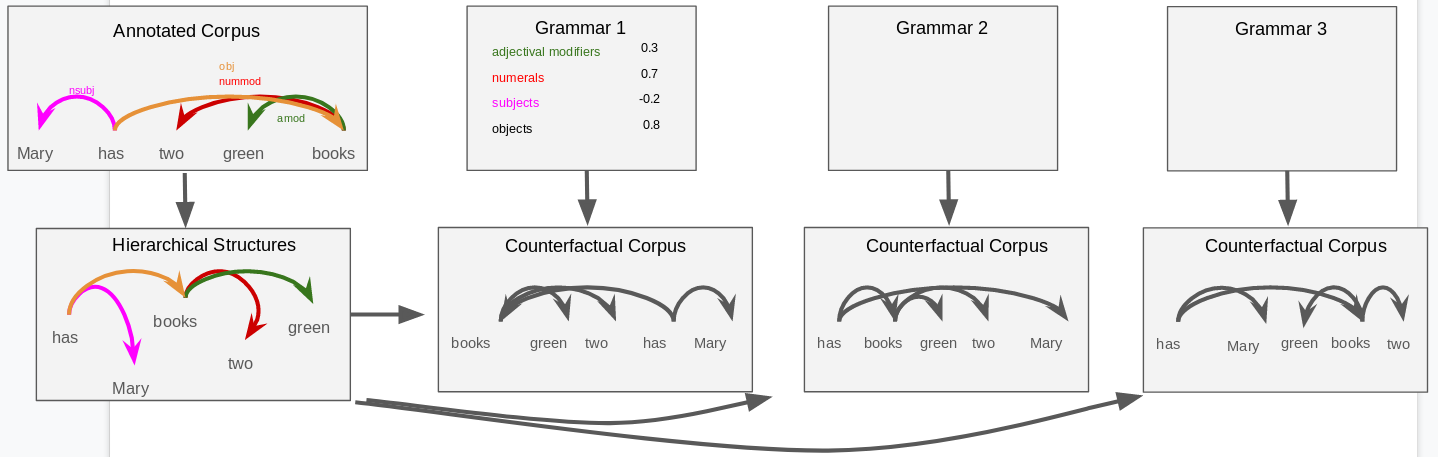
\includegraphics[width=\textwidth]{figures-gdrive/counterfactual-languages.png}
	\caption{\note{Can say more here to explain how it works} Estimating chance by constructing counterfactual grammars and languages.\jd{this figure is again blurry for me. also looks like there's sth in the background on the left?}}\label{fig:grammars}
\end{figure}


Universal Dependencies 2.4 defines 37 universal syntactic relations that are used to label dependency arcs across all corpora.
These relations encode cross-linguistically meaningful relations such as subjects, objects, and adjectival modifiers.
We define ordering grammars by assigning a parameter $a_\tau \in [-1,1]$ to every one of these 37 universal syntactic relations.
Relations sometimes have language-specific subtypes; we do not distinguish these subtypes.

Following Gildea and colleagues, this parameter defines how dependents are ordered relative to their head:
Given a head and a set of dependents, we order each dependents by the parameter $a_\tau$ assigned to the syntactic relation linking it to the head.
Dependents with negative weights are placed to the left of the head; dependents with positive weights are placed to the right.

Ordering grammars describe languages that have consistent word order:
For instance, the subject is consistently ordered before or after the verb, depending on whether the parameter for the verb-subject dependency is positive or negative.

We construct baseline grammars by randomly sampling the parameters $a_\tau$.
Such baseline grammars define languages that have consistent word order, but do not exhibit systematic preferences for specific word order patterns such as short dependencies.


In actual languages, the ordering of words is largely determined by the syntactic relations (CITE).
However, certain kinds of rules cannot be modeled by our word order grammars, such as rules sensitive to the category of the dependent (e.g., differences between nominal and pronominal objects).
Word order freedom also is not modeled.
In this sense, ordering grammars represent approximations to the kinds of ordering rules found in natural language \citep{gildea-optimizing-2007, gildea-grammars-2010, gildea-human-2015}.
See Section (Discussion) for further discussion.


We first constructed at least 10 baseline grammars for each of the 54 real languages.
We then continued to construct baseline grammars until a precision-based stopping criterion was reached (CITE). This criterion was designed to ensure that enough grammars were sampled to reliably compare the tradeoff curves of real and baseline grammars, without biasing results towards or against our hypothesis (see SI).

\subsection{Results}

\begin{figure}
	\begin{center}
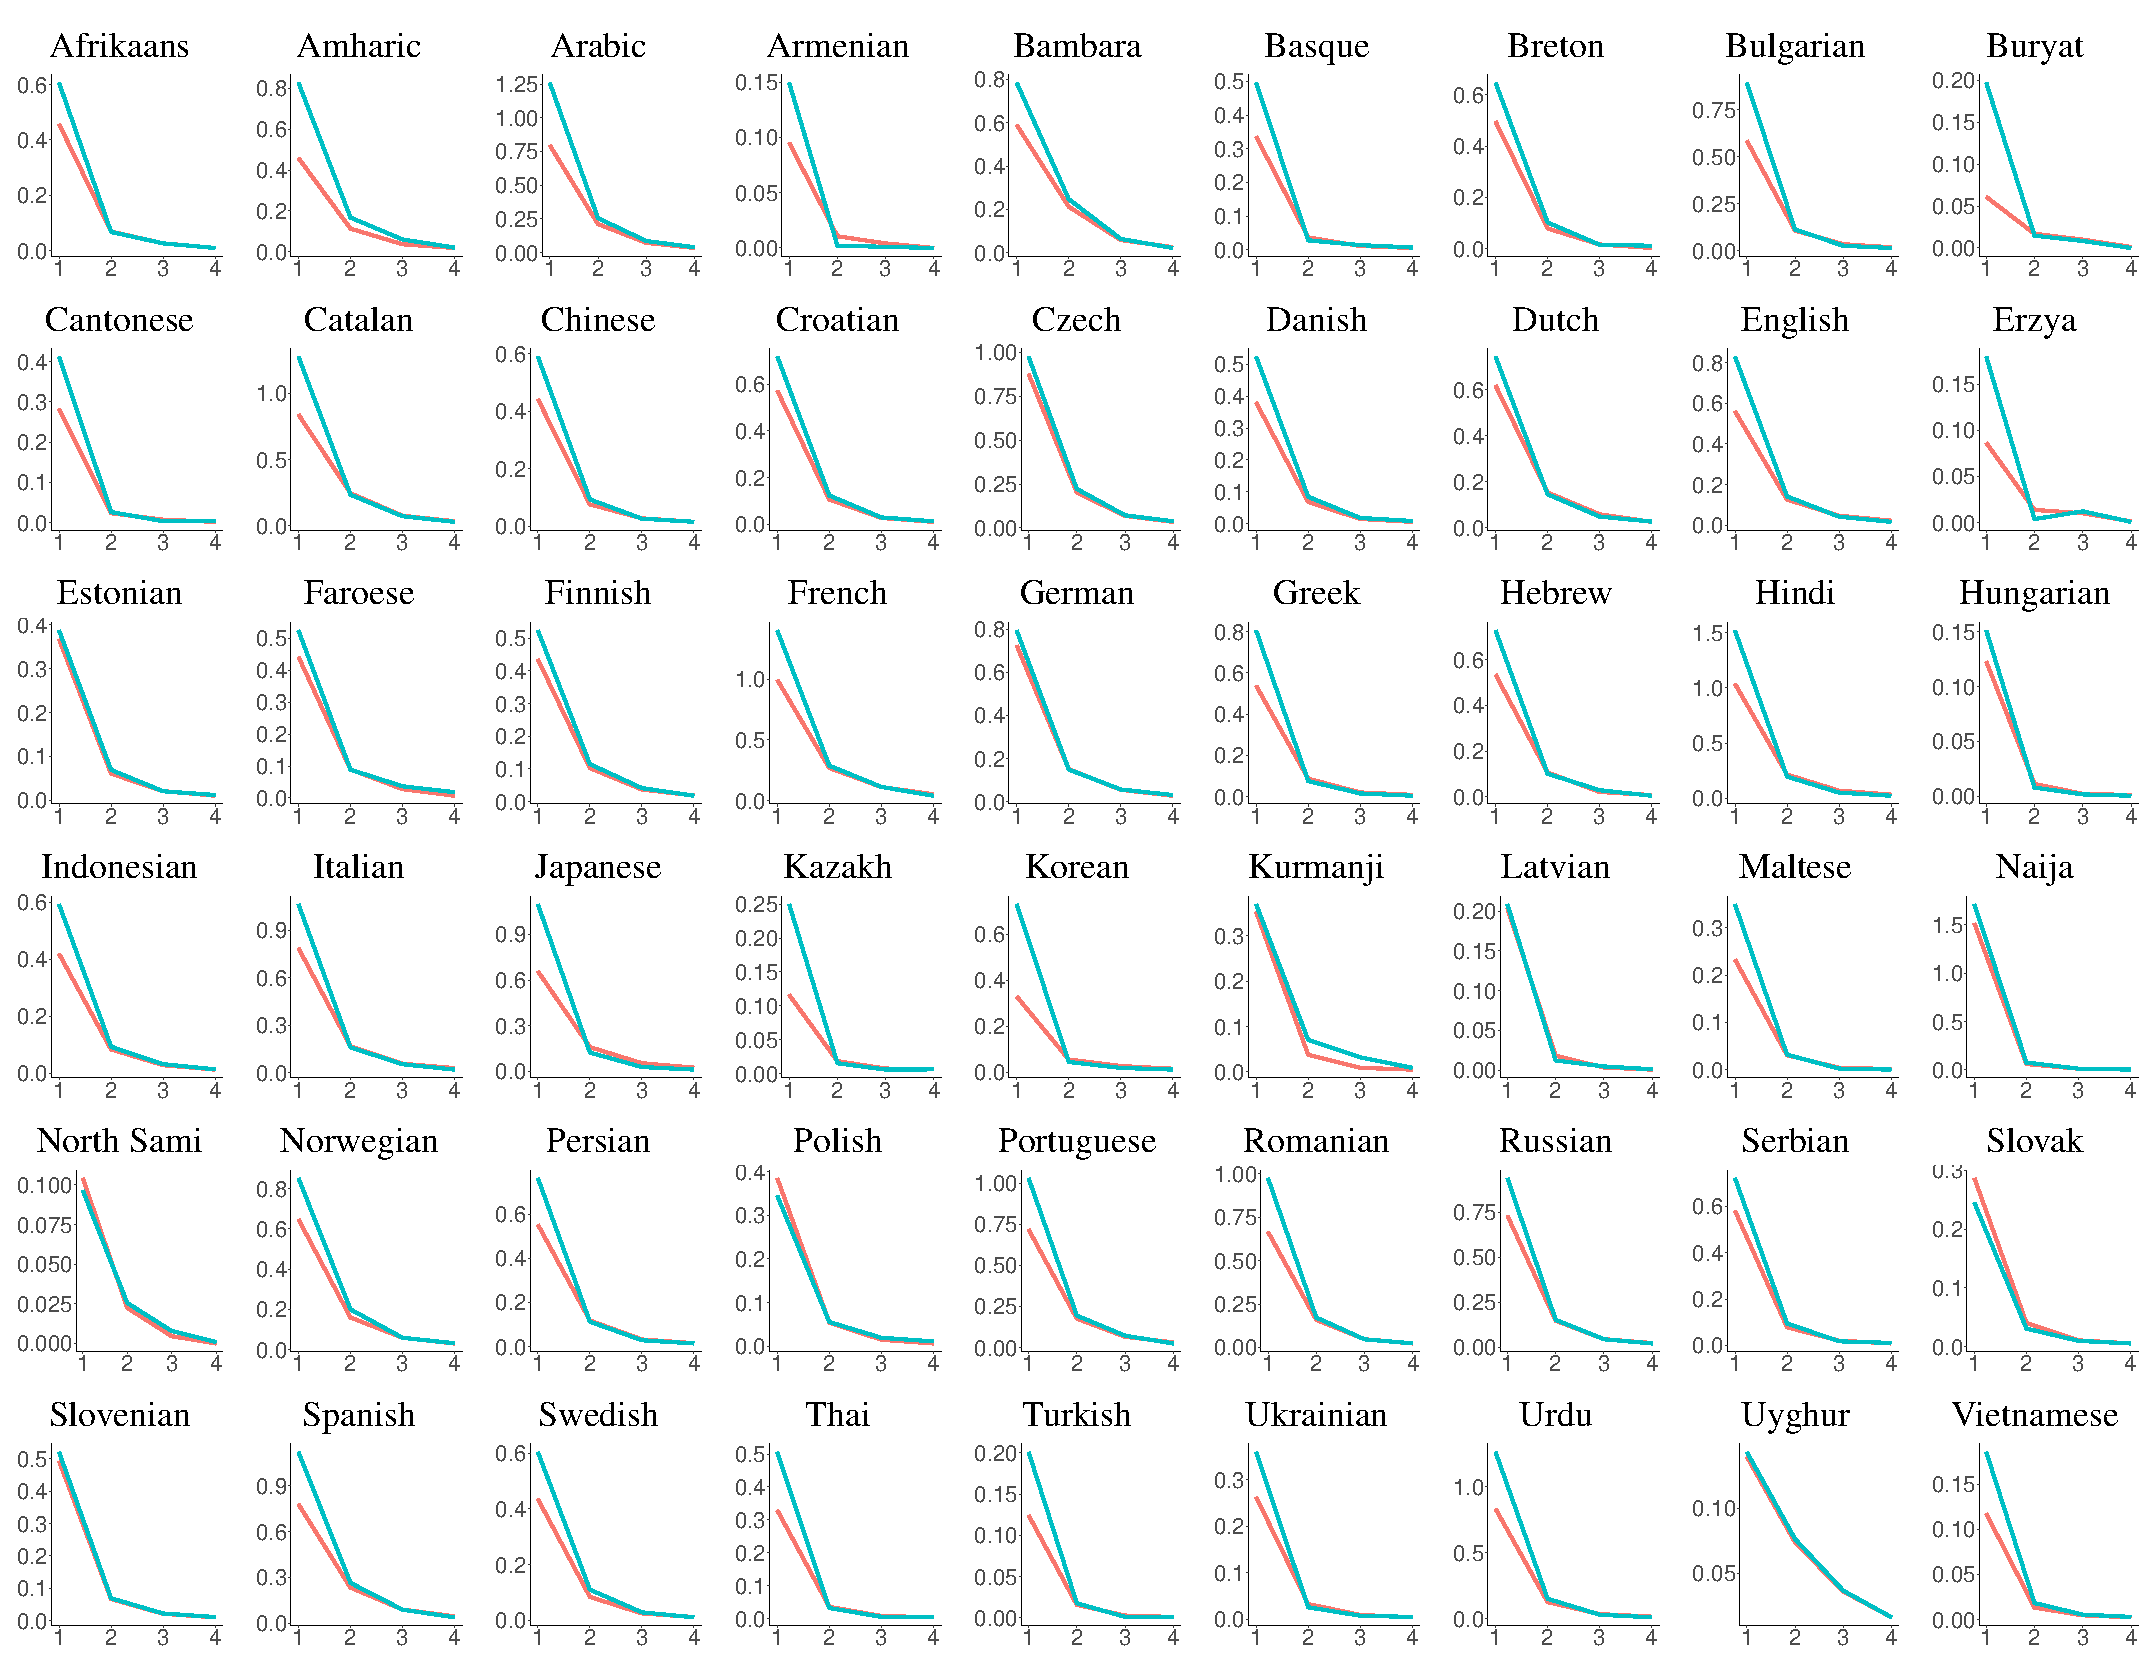
\includegraphics[width=\textwidth]{it-table.pdf}
\end{center}
	\caption{$I_t$ (y-axis) as a function of $t$ (x-axis), for real (blue) and counterfactual (red) orders. We plot the median over all runs of the neural network estimator, and over all random grammars.}\label{fig:it}
\end{figure}



\begin{figure}
	\begin{center}
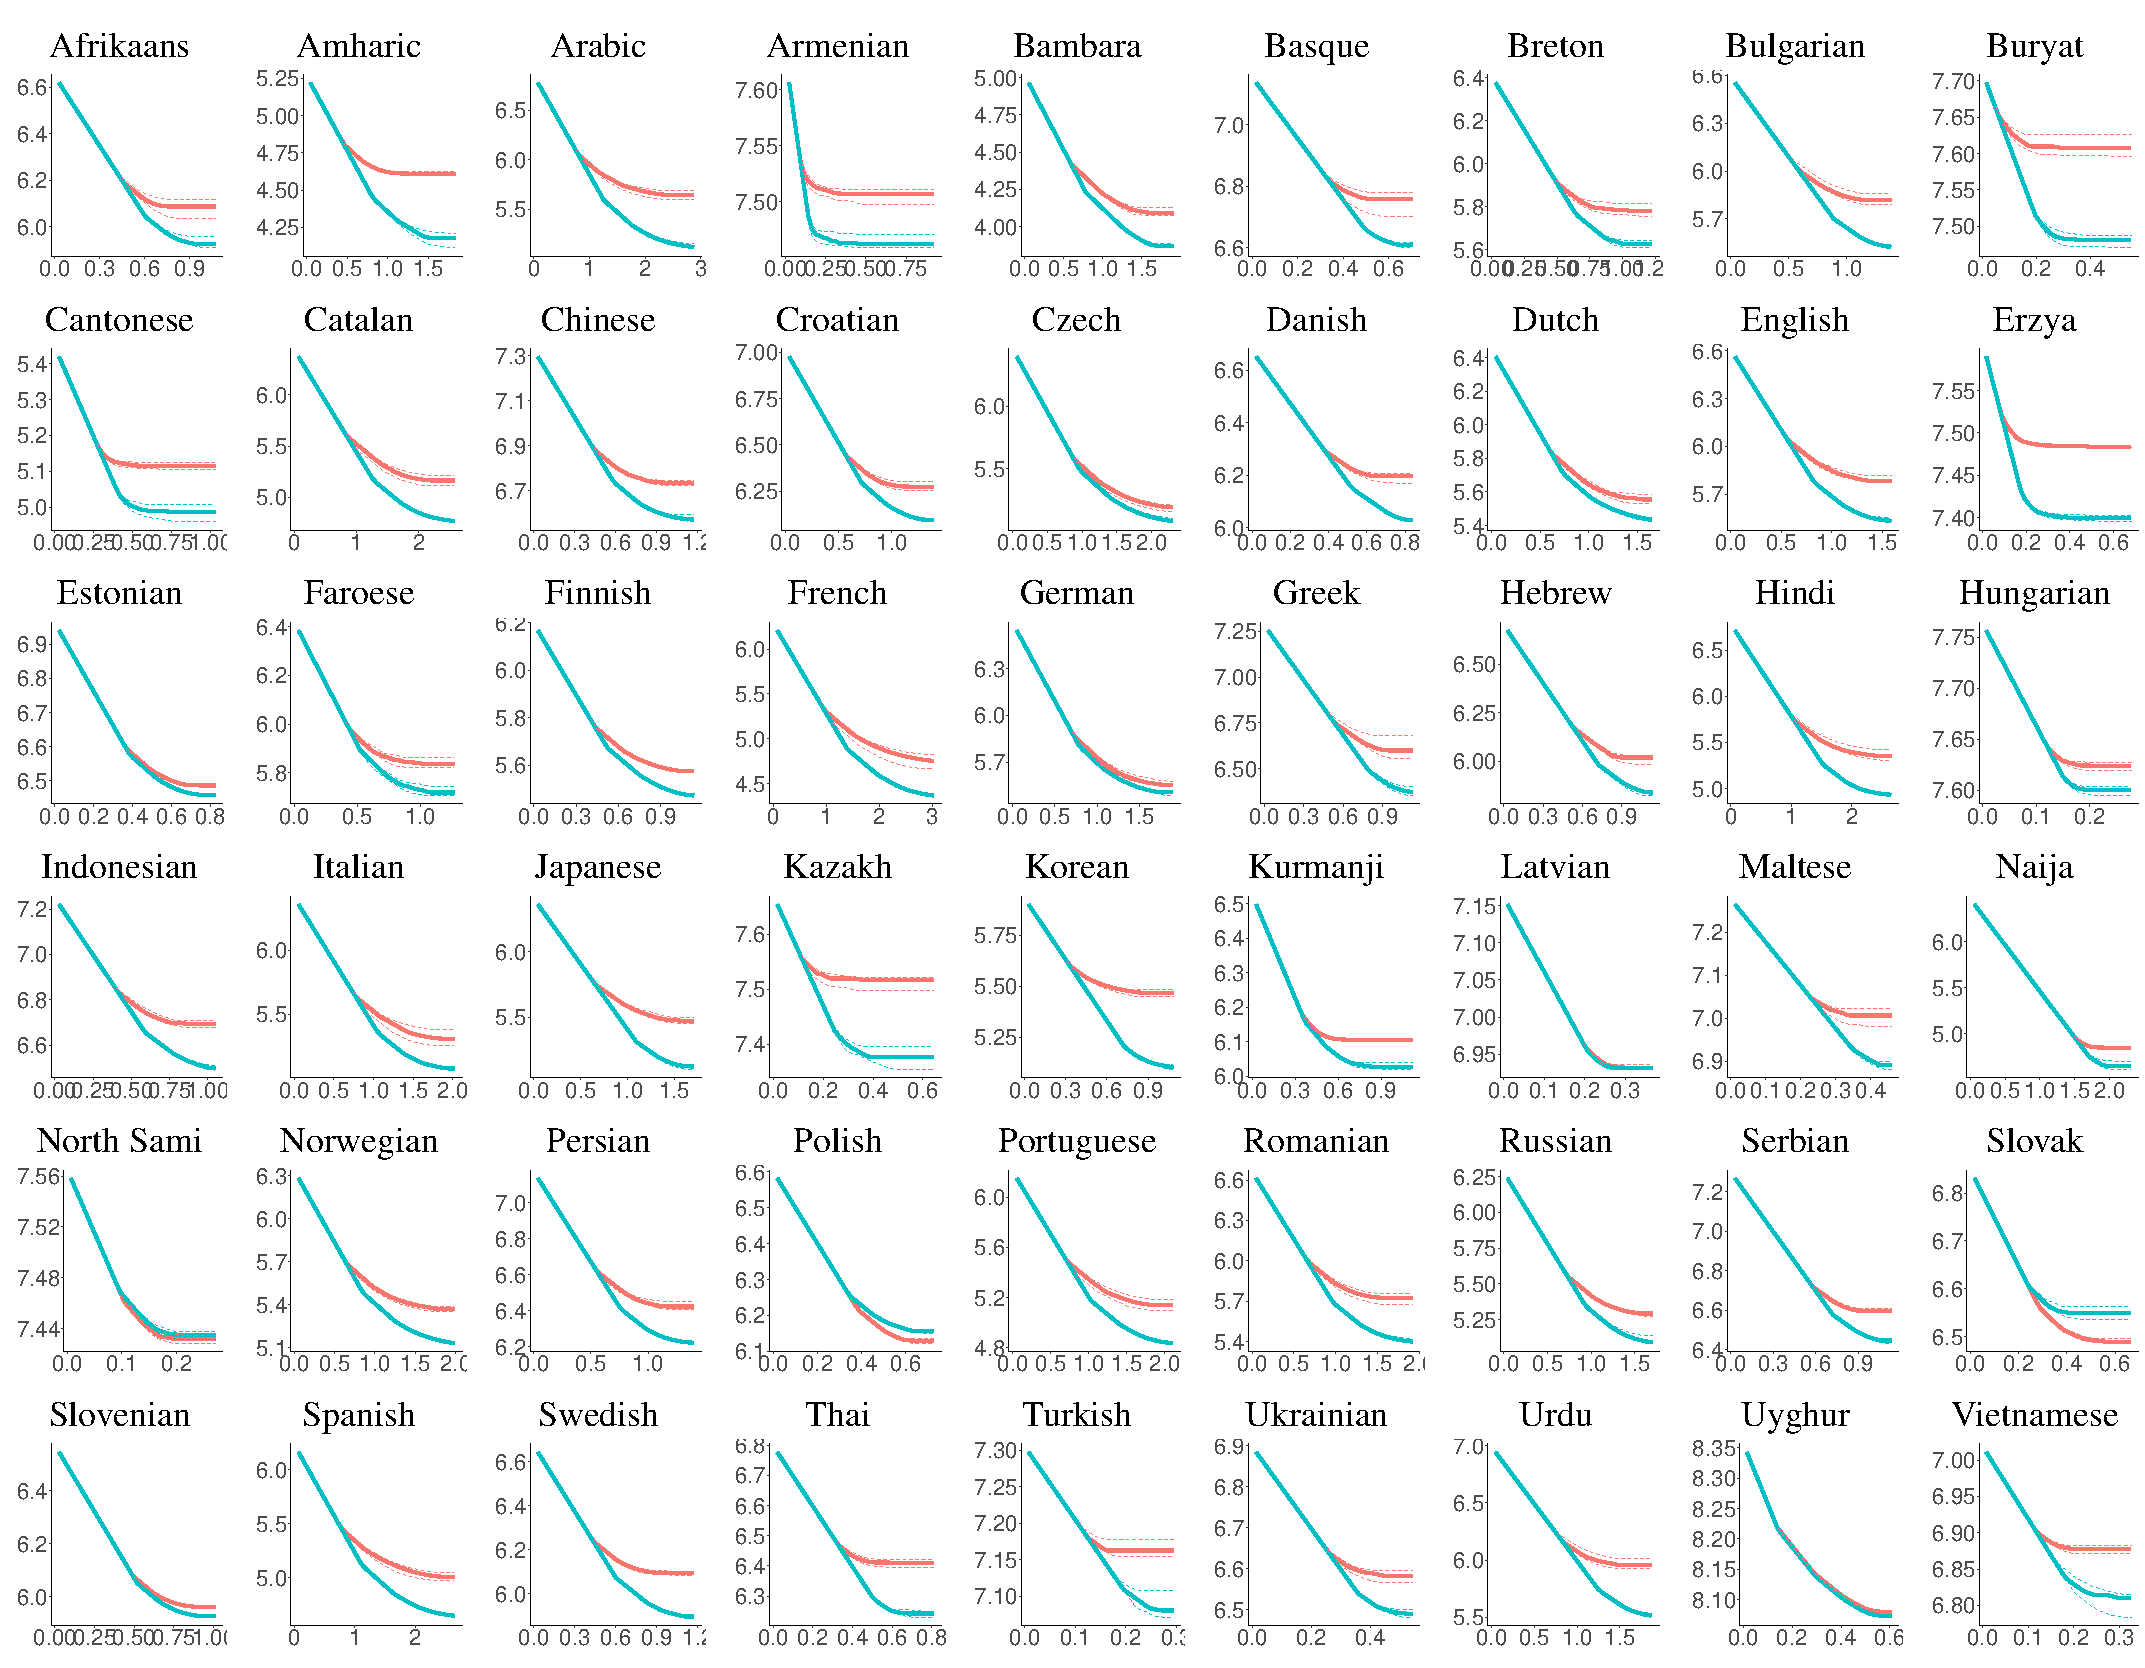
\includegraphics[width=\textwidth]{results-table.pdf}
\end{center}
	\caption{Median surprisal (y-axis) at given memory level (x-axis), for real orders (blue) and random baseline grammars (red). We provide 95\% confidence bands. These are computed over different runs of the estimation algorithm for the real orders, and over different runs \emph{and} different grammars for the baseline grammars.}\label{fig:median-table}
\end{figure}


\begin{figure}
	\begin{center}
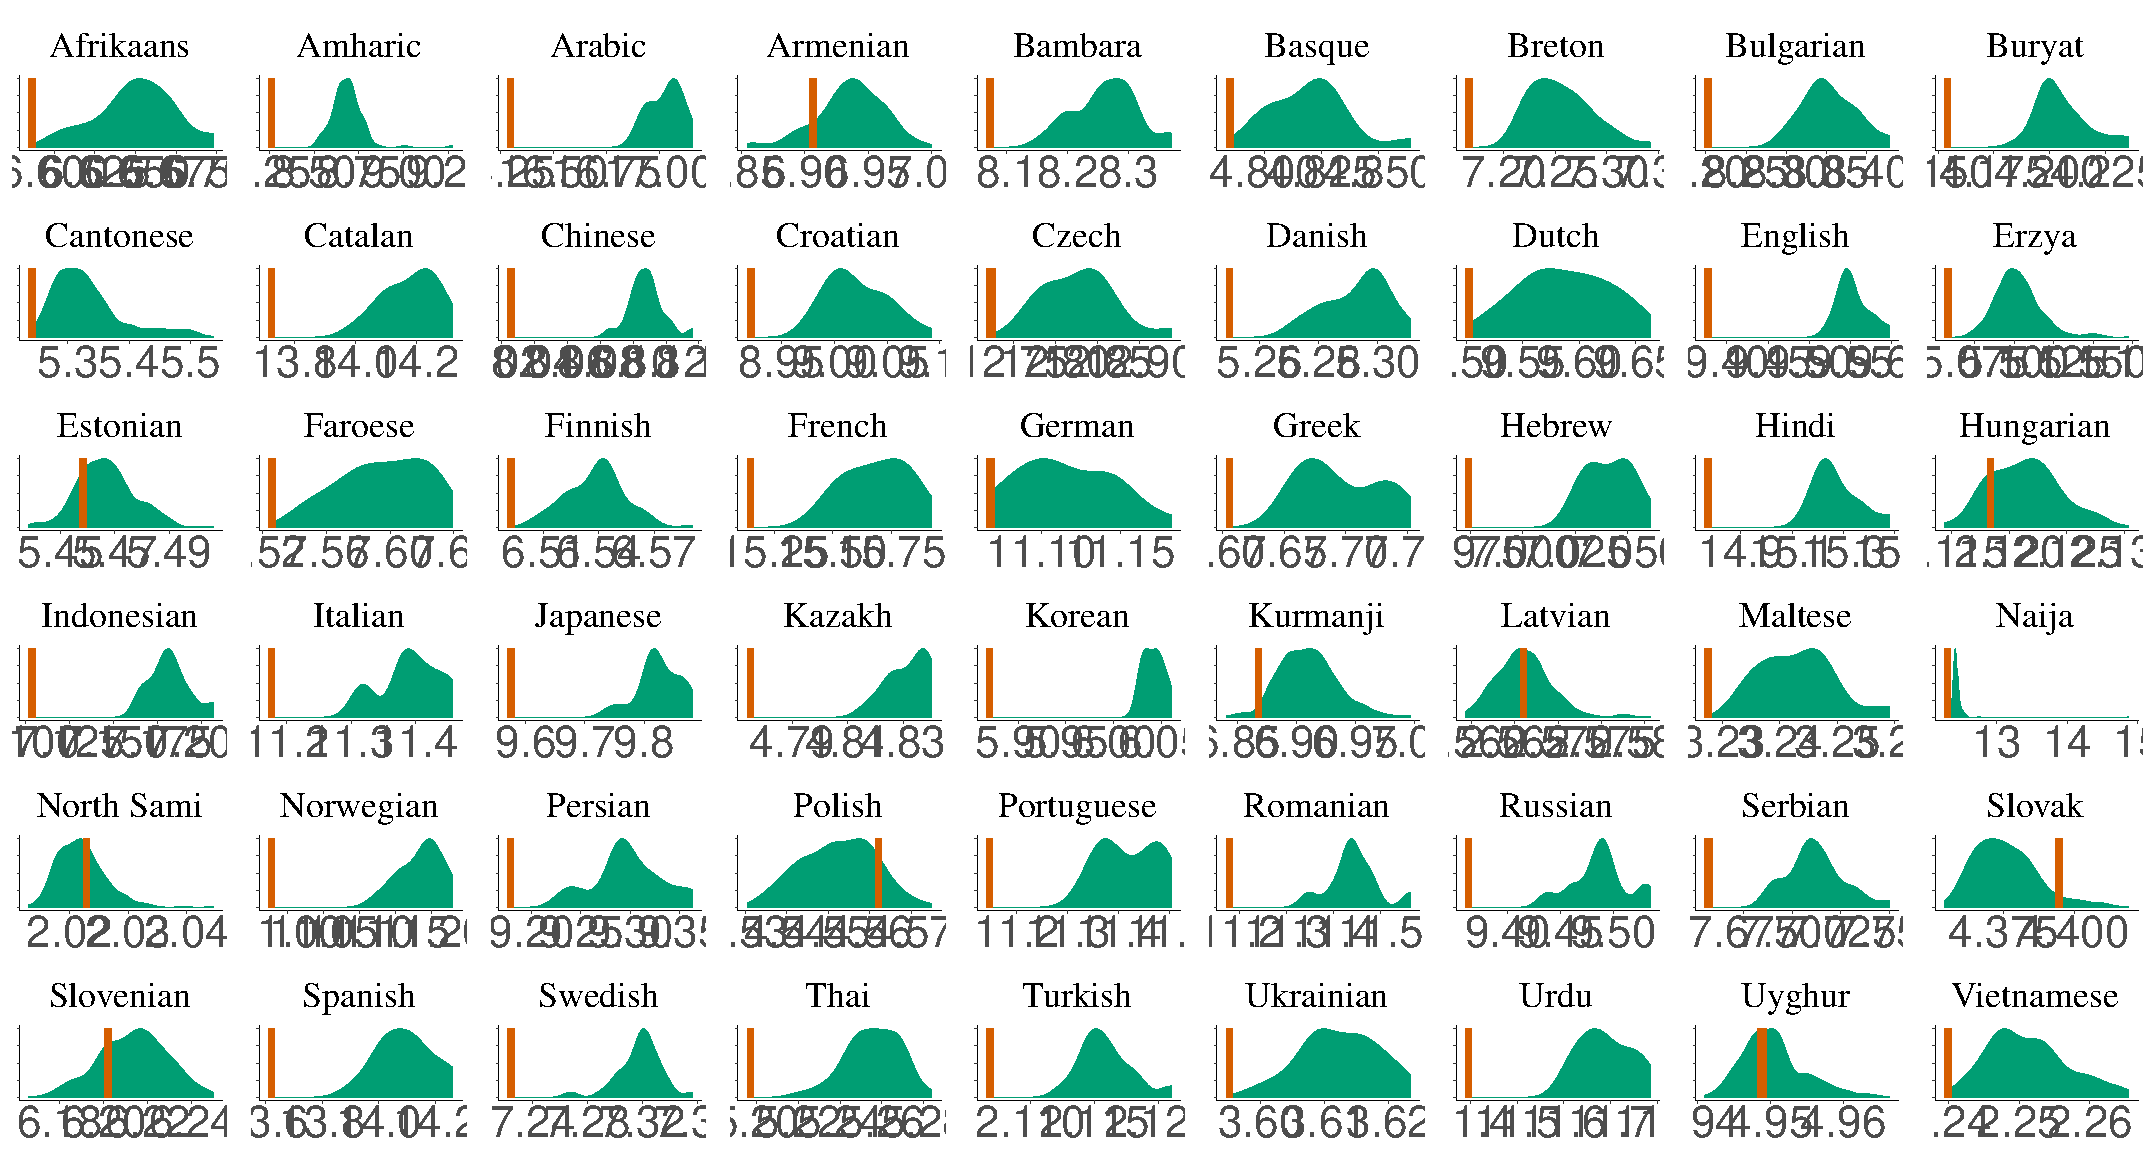
\includegraphics[width=\textwidth]{auc-table.pdf}
\end{center}
	\caption{AUC Histograms}\label{fig:auc}
\end{figure}





%The numbers of samples taken per language are provided in SI Table~\ref{tab:samples}.

%In Figure~\ref{tab:plain-results} (TODO), we show the estimated memory-surprisal tradeoff curves for all samples.


In Figure~\ref{fig:it}, we show the estimated values of $I_t$ for real orders (blue) and the median of $I_t$ across different baseline grammars (red).
In most languages, $I_1$ is distinctly larger for the actual orderings (blue) compared to the baseline orderings (red). This means that real orderings tend to concentrate more predictive information at the immediately preceding word than baseline grammars.

In Figure~\ref{fig:median-table}, we show the resulting bounds on the memory-surprisal tradeoff curves, showing median surprisals at given levels of memory, for real and baseline languages.
We compute surprisal at 40 evenly spaced points of memory (selected individually for each language), over real orders and baseline grammars.
We then compute the median surprisal over all runs for the real language, and over all baselines grammars.
For each point, we compute a confidence interval for the median surprisal, using the binomial PDF. \mhahn{some standard stats reference}
This is an \emph{exact} confidence interval, without parametric assumptions or asymptotic approximations.

Numerically, the real language provides better tradeoffs than the median of the baselines across languages, with four exceptions (Latvian, North Sami, Polish, Slovak).


In order to quantify the degree of optimality of real orders, we further computed the area under the memory-surprisal tradeoff curve (AUC) for real and baseline orderings.
Area under the curve (AUC) is a general quantity evaluating the efficiency of a tradeoff curve (CITE).
A \emph{smaller} area indicates a \emph{more efficient} tradeoff.
In Figure~\ref{fig:auc}, we plot the AUC for the real orderings, together with the distribution of AUCs for baseline grammars.
Numerically, the AUC is smaller in the real orderings than in at least 50\% of baseline grammars in all but four languages

%\subsection{Statistical Analysis}

%We now describe how we compared memory-surprisal tradeoffs between real and baseline languages.
%We want to test whether languages' surprisal-memory tradeoffs better than those of most baseline languages.
%We compare real and baseline languages by evaluating which languages result in lower surprisal at the same level of memory.
%We now describe the statistics we use to quantifying the difference between real and baseline languages.
%We do everything in a frequentist framework (null hypothesis testing \& confidence intervals), as we can do exact tests and confidence intervals without parametric assumptions.
%\mhahn{Maybe we can explain how the tests \& CIs also have reasonable Bayesian interpretations (for the specific methods used here, rejection of the null should guarantee that the posterior of the null hypothesis is small under a wide range of priors.).}

%\paragraph{Median Surprisal and Confidence Interval for Medians}



%\paragraph{CI for Median Difference}
%We create (nonparametric and nonasymptotic) confidence interval for the difference between real and baseline median surprisals at each memory value.
%\mhahn{the resulting plots are not very intuitive, might scrap this}
%
%% yStudyTradeoff_Bootstrap_Parallel_OnlyWordForms_BoundedVocab_BinomialTest_Single_MedianDiffCI.py



%This statistic also should have a reasonable Bayesian interpretation:
% E.g., if the random samples are unimodal, and we do inference over only the median (location family), 



%\begin{figure}
%	\begin{center}
%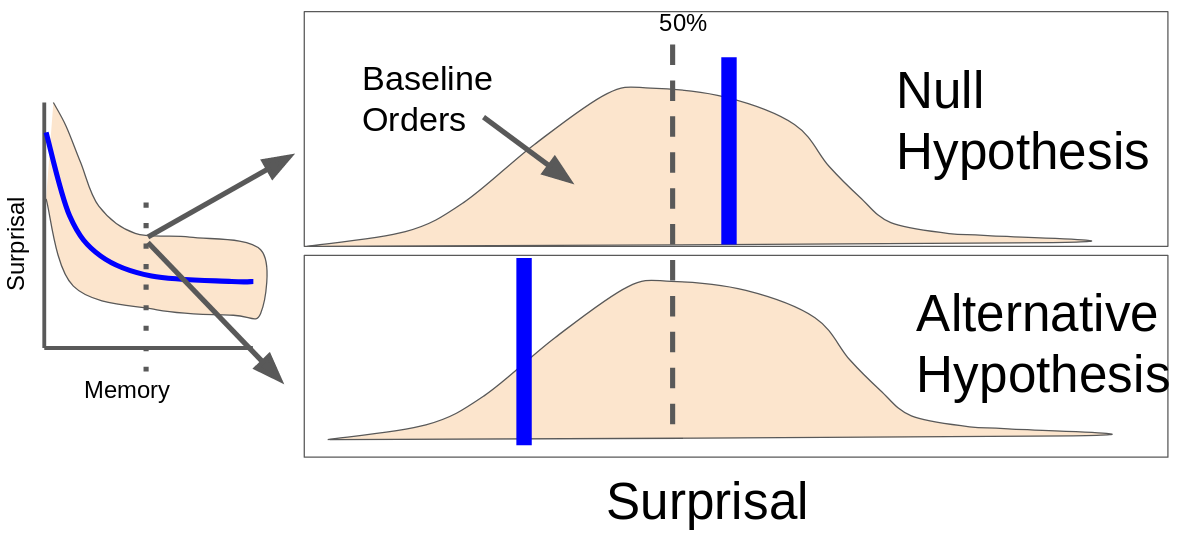
\includegraphics[width=0.45\textwidth]{figures/nhst.png}
%\end{center}
%	\caption{Illustration for the pointwise null-hypothesis significance test. At a given level of memory, we test against the null hypothesis that at least half of the baseline orders provide lower surprisal than the real language.}\label{fig:nhst-pointwise}
%\end{figure}






%For each memory value $\mu$, we do a significance test (nonparametric and nonasymptotic).
%\begin{equation}
%	W_+(\mu) \geq W_-(\mu)
%\end{equation}
%We use the empirical median for the real language.

% yStudyTradeoff_Bootstrap_Parallel_OnlyWordForms_BoundedVocab_BinomialTest_Single.py

%We take the REAL values to be estimated exactly by their medians.

%TODO some aggregate visualization of the quantiles
%\paragraph{AUC}
%TODO some aggregate visualization

%\begin{figure}
%	\begin{center}
%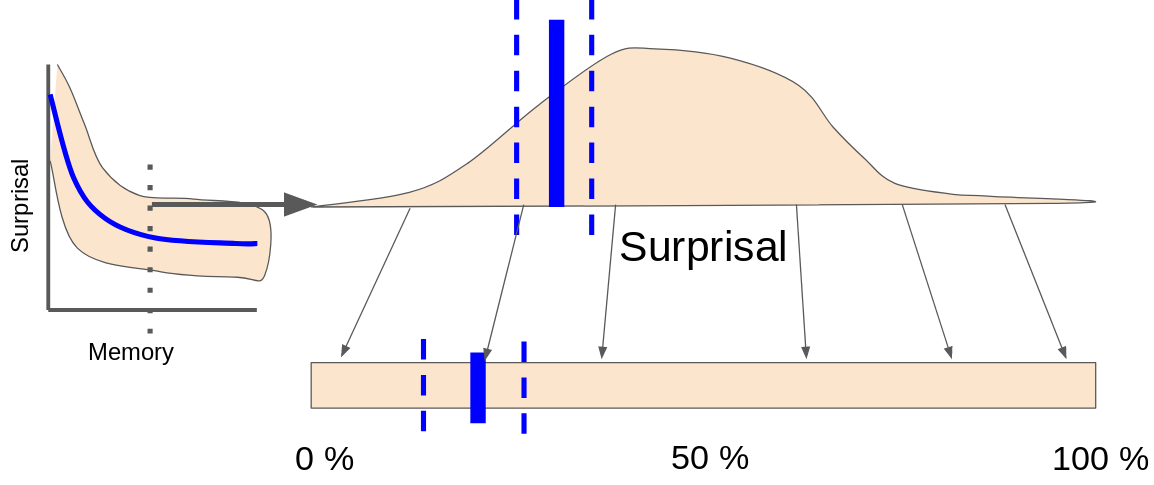
\includegraphics[width=0.45\textwidth]{figures/quantile.png}
%\end{center}
%	\caption{Illustration for the quantile estimate. At each level of memory, we provide an estimate of the percentage of baseline languages that have lower surprisal than the real language.}\label{fig:quantile-pointwise}
%\end{figure}



%Also the following does not assume unimodality, and ends up getting about the same intervals
%% yStudyTradeoff_Bootstrap_Parallel_OnlyWordForms_BoundedVocab_BinomialTest_Single_UnimodalBoundOnQuantile_BothDirections_NoAssumption.py






%In Figure~\ref{tab:slice-hists-real}, we show the distribution of surprisals achieved at the maximal memory value for real and random languages.

%In Figure~\ref{fig:hist-real}, we show surprisals at maximum memory, after z-transforming for each individual language and then aggregating.

%In Table \ref{tab:median_diffs}, we show the differences in median surprisal, as a function of memory.


%In Table~\ref{tab:boot-g}, we report the bootstrap estimates and confidence intervals for G~(\ref{eq:g}).
%$\E[G]$ was not estimated to be significantly above $>5$ for four languages: Latvian, North Sami, Polish, and Slovak.


%In Table~\ref{tab:quantiles}, we show the quantiles.





\subsection{Discussion}

We have found that 50 out of 54 languages provide better memory-surprisal tradeoffs than random baselines with consistent but counterfactual word order rules.

Four languages provide exceptions; these are Latvian (Baltic), North Sami (Uralic), Polish and Slovak (both Slavic).
All four languages have strong word order freedom (CITE).
Freedom of word order plausibly makes sentences less predictable, as the same syntactic structure can receive different surface realizations.
We thus hypothesized that freedom of word order impacts the memory-surprisal tradeoff, and that languages with more strongly fixed word order should display more optimal memory-surprisal tradeoffs.

To test this hypothesis, we examined the correlation between word order freedom and the surprisal difference between real and baseline orderings.
To quantify word order freedom, we used a corpus-based estimate, the \emph{branching direction entropy}~\citep{futrell-quantifying-2015}.
This is the entropy of the ordering (head-first or dependent-first) of dependencies conditioned on the dependency label and the part-of-speech label of head and dependent.
These two quantities are plotted in Figure~\ref{fig:hist-real}.
We found that branching direction entropy was strongly correlated with the surprisal difference between real and baseline orderings (Spearman correlations -0.58, $p = 7.414e-6$).

We will address this in Experiment 3.


\begin{figure}
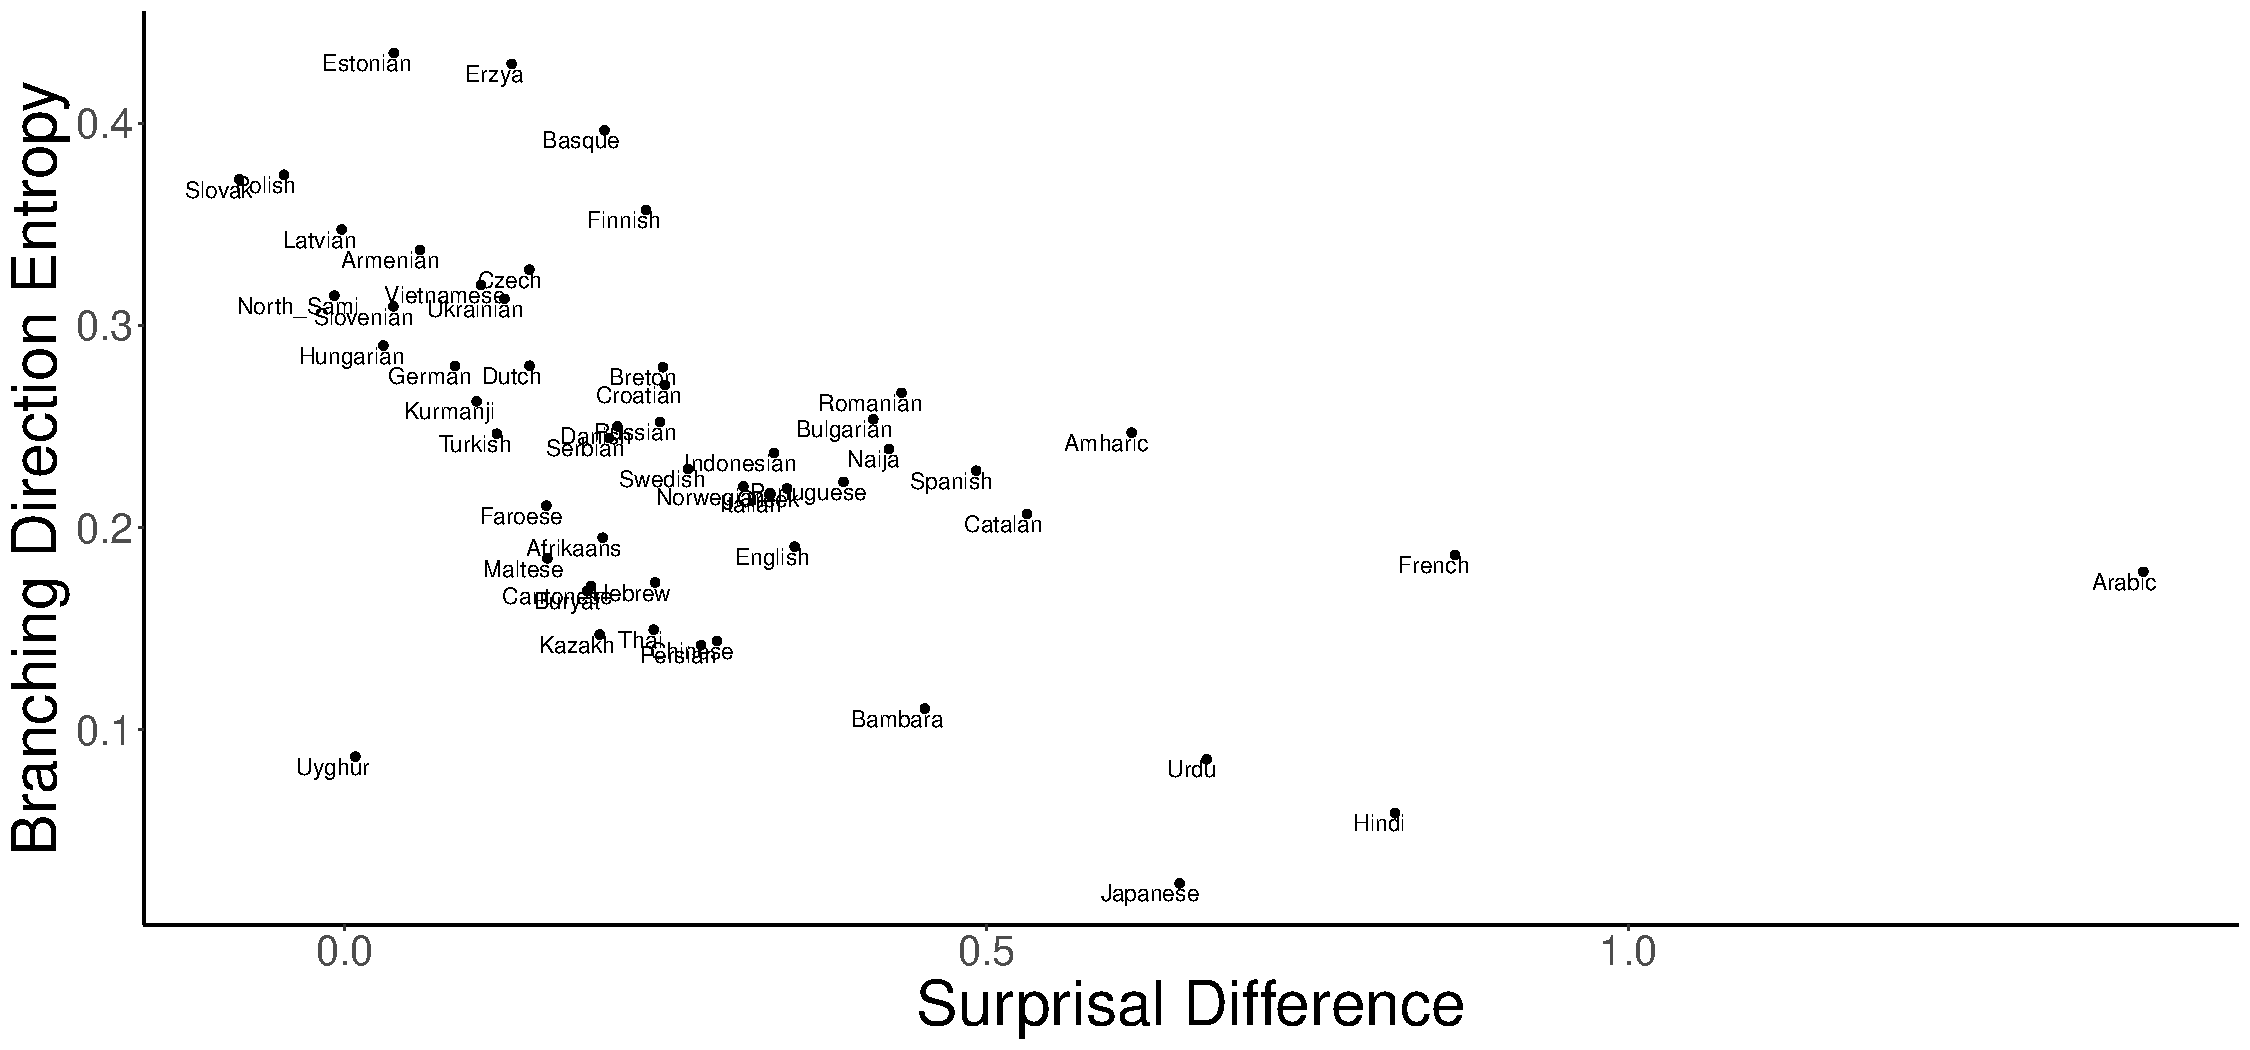
\includegraphics[width=0.95\textwidth]{figures/surprisal-branching-entropy-REAL.pdf}
	\caption{Surprisal Difference vs Branching Direction Entropy.}\label{fig:hist-real}
\end{figure}


\mhahn{One thing that has to be discussed: the absolute values differ between languages}



A possible concern is that the optimization observed in Experiment 1 might be an artifact of the grammar formalism.
We will address this in Experiment 3.
%To address this possibility, we repeated the experiment comparing baseline grammars to grammars that represent the word order of the real languages as faithfully as is possible with the grammar formalism.




\subsection{Controlling for Information Structure}\label{subsec:freedom}



We now address the questions raised in Section~\ref{subsec:expt2-discussion}.
First, we compare memory-surprisal tradeoffs for grammars approximating real orders in the same formalism as the baseline grammars (Section~\ref{sec:compare-mle}).
Second, we draw on a corpus of Czech with information structure annotation to determine whether real orders are more optimized when comparing to baselines taking information structure into account (Section~\ref{sec:czech}).


\subsubsection{Comparing Grammars Fitted to Actual Orders}\label{sec:compare-mle}

As discussed in Section~\ref{subsec:expt2-discussion}, there is the possibility of a confound in the fact that baselines are constructed using a grammar formalism that is in some ways too restrictive to model all word order rules found in natural languages.
To ensure that results are not due to the representational restrictions of the word order grammar formalism, we compare the real languages to the result of ordering the corpora according to grammars that approximates the observed orders to the extent possible in the grammar formalism.
These grammars have exactly the same representational constraints as the baseline grammars.
Importantly, they differ from real languages in having entirely deterministic order.
We expect these grammars to have better memory-surprisal tradeoffs than comparable random baseline grammars across all languages.

We create ordering grammars that are fit to the actual orderings of each language.
These grammars faithfully represent the ordering rules if the actual language, to the extent that is possible in the formalism of ordering grammars.
These grammars are extracted from the observed orders using the method of \cite{hahn2020universals}.
We compared the memory-surprisal tradeoffs of these extracted grammars to the same baseline grammars as above.


\paragraph{Results}


We show estimated memory-surprisal tradeoffs in Figure~\ref{fig:median-table}, and histograms of the area under the tradeoff curve (AUC) in Figure~\ref{fig:auc-mle}.
The AUC for the fitted grammars is lower than more than 50\% of random baseline grammars in all 54 languages ($p < 0.01$, using two-sided Binomial test and Hochberg's step-up procedure).

Thus, the ordering regularities of real languages provide more efficient tradeoffs than most possible order grammars also when comparing within the same word order grammar formalism.

\begin{figure}
	\begin{center}
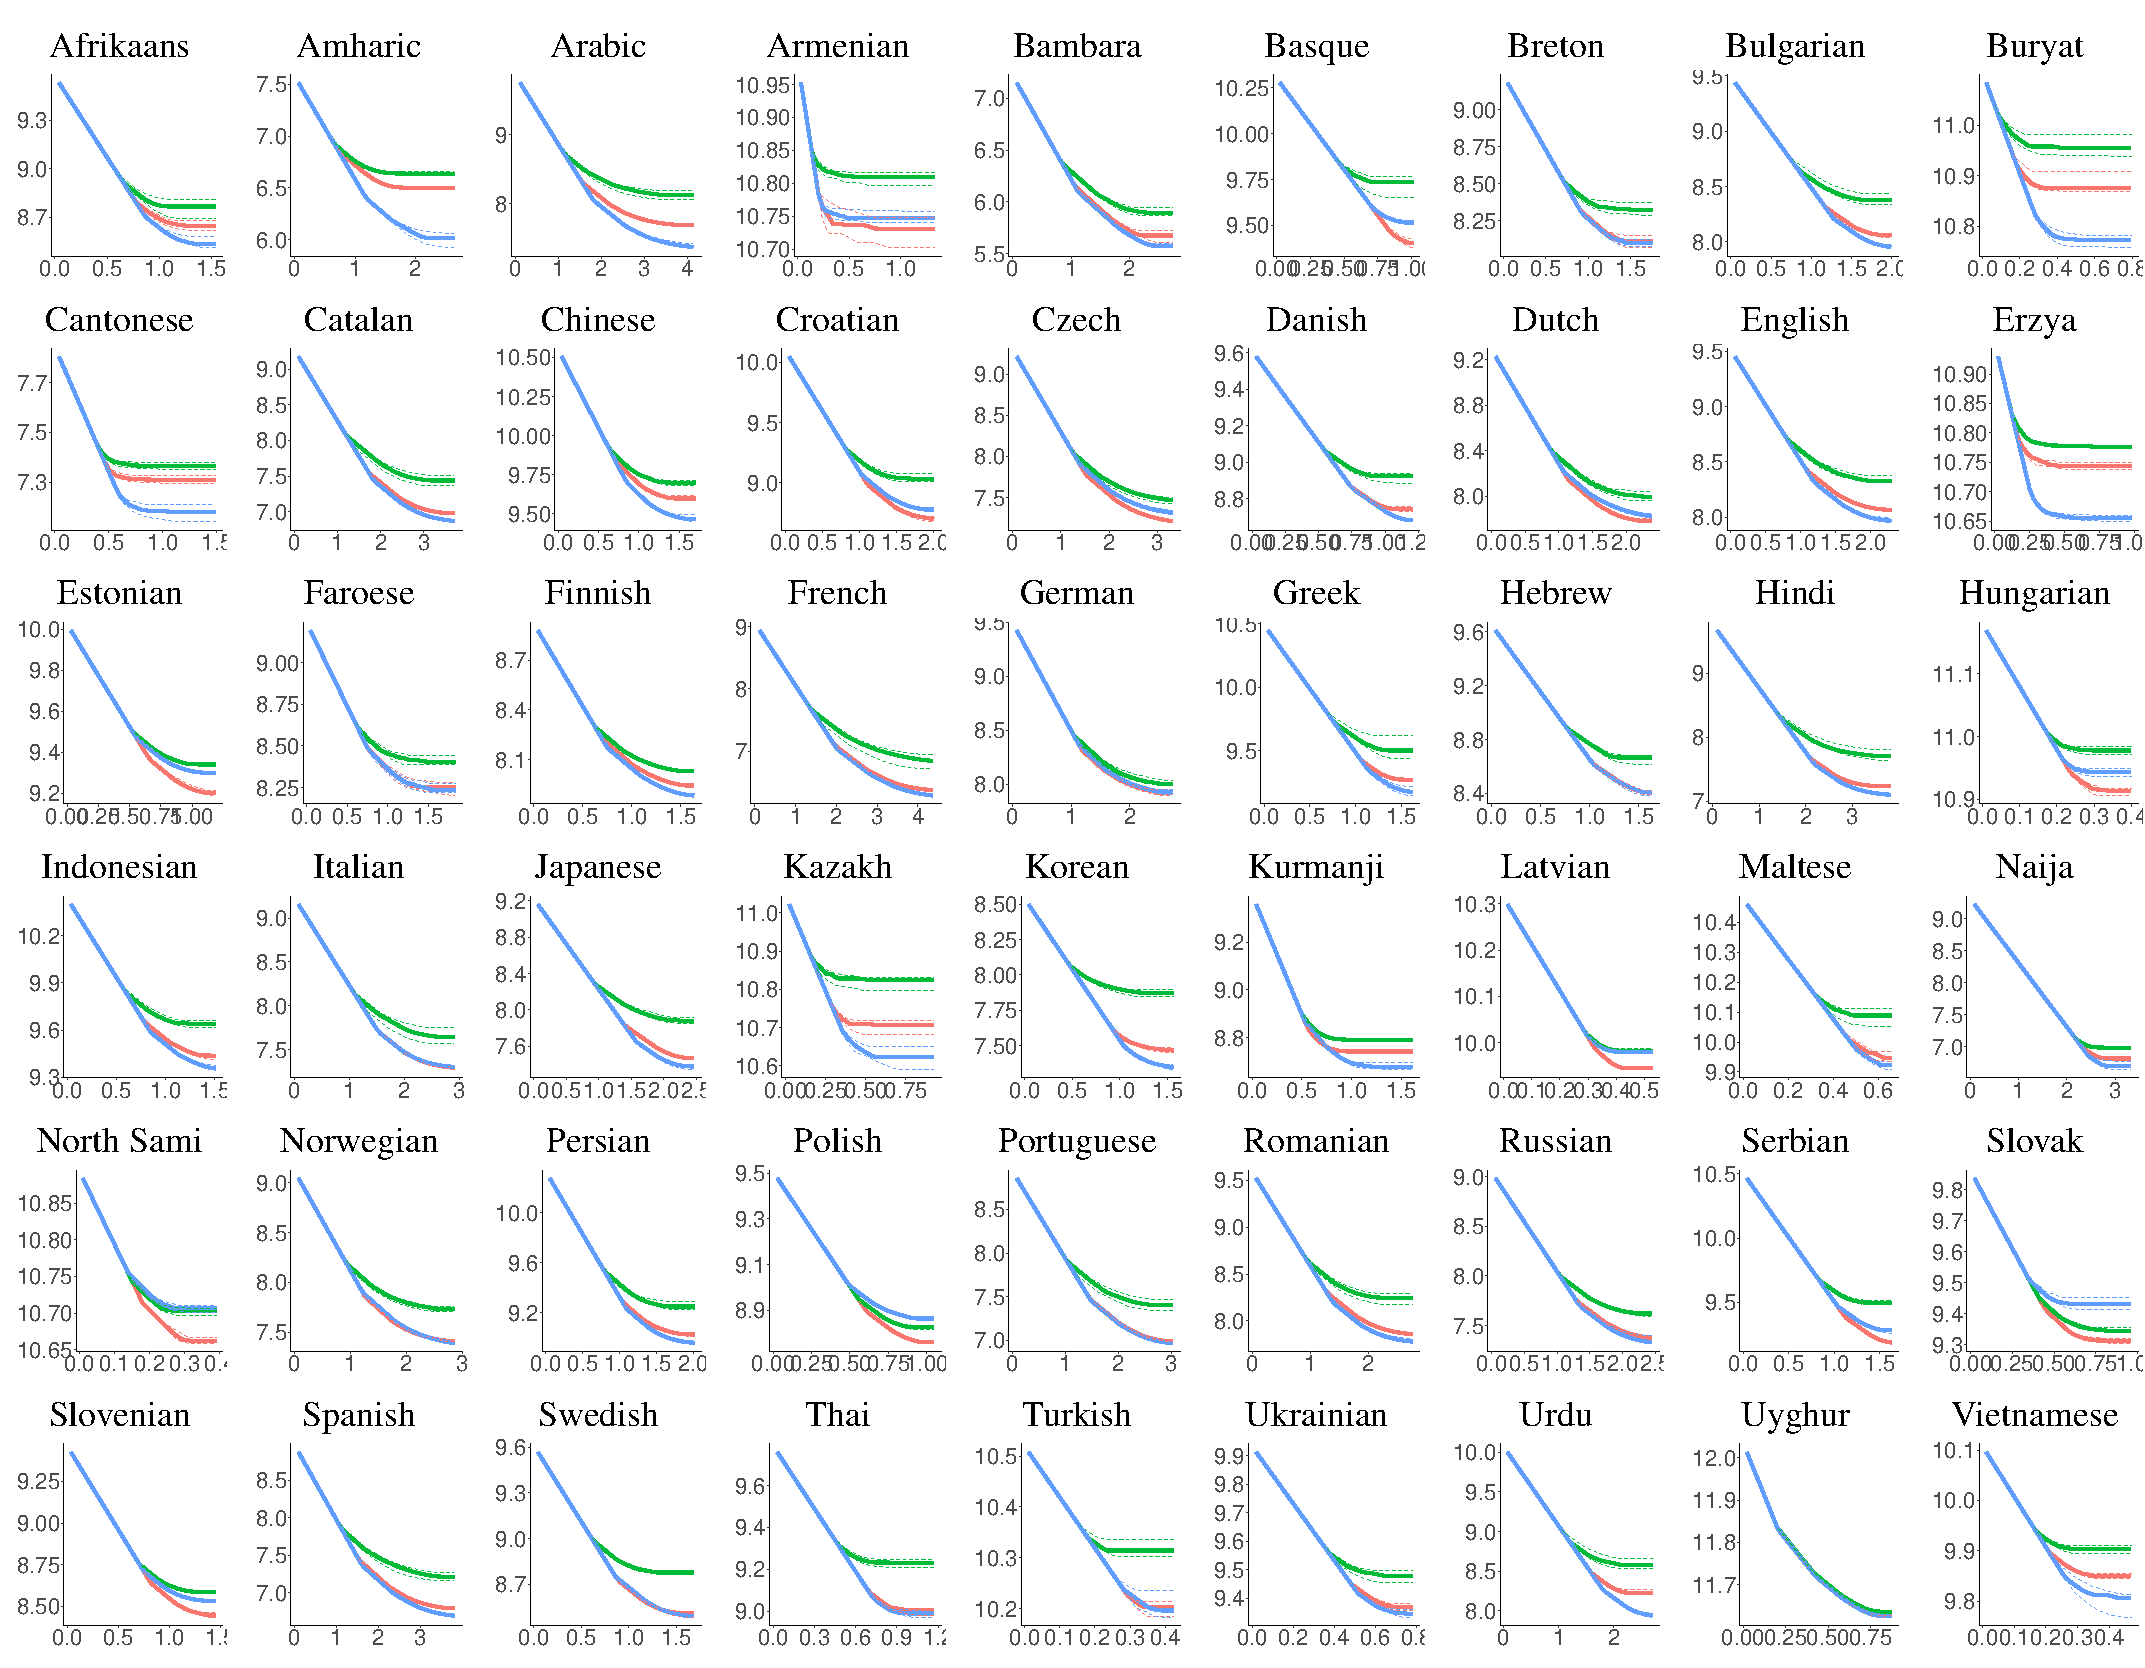
\includegraphics[width=\textwidth]{results-table-mle.pdf}
\end{center}
	\caption{Median surprisal (y-axis) at given memory level (x-axis), for real orders (blue) and random baseline grammars (red). We provide 95\% confidence bands. These are computed over different runs of the estimation algorithm for the real orders, and over different runs \emph{and} different grammars for the baseline grammars. \mhahn{make axis numbers readable}}\label{fig:median-table}
\end{figure}



\begin{figure}
	\begin{center}
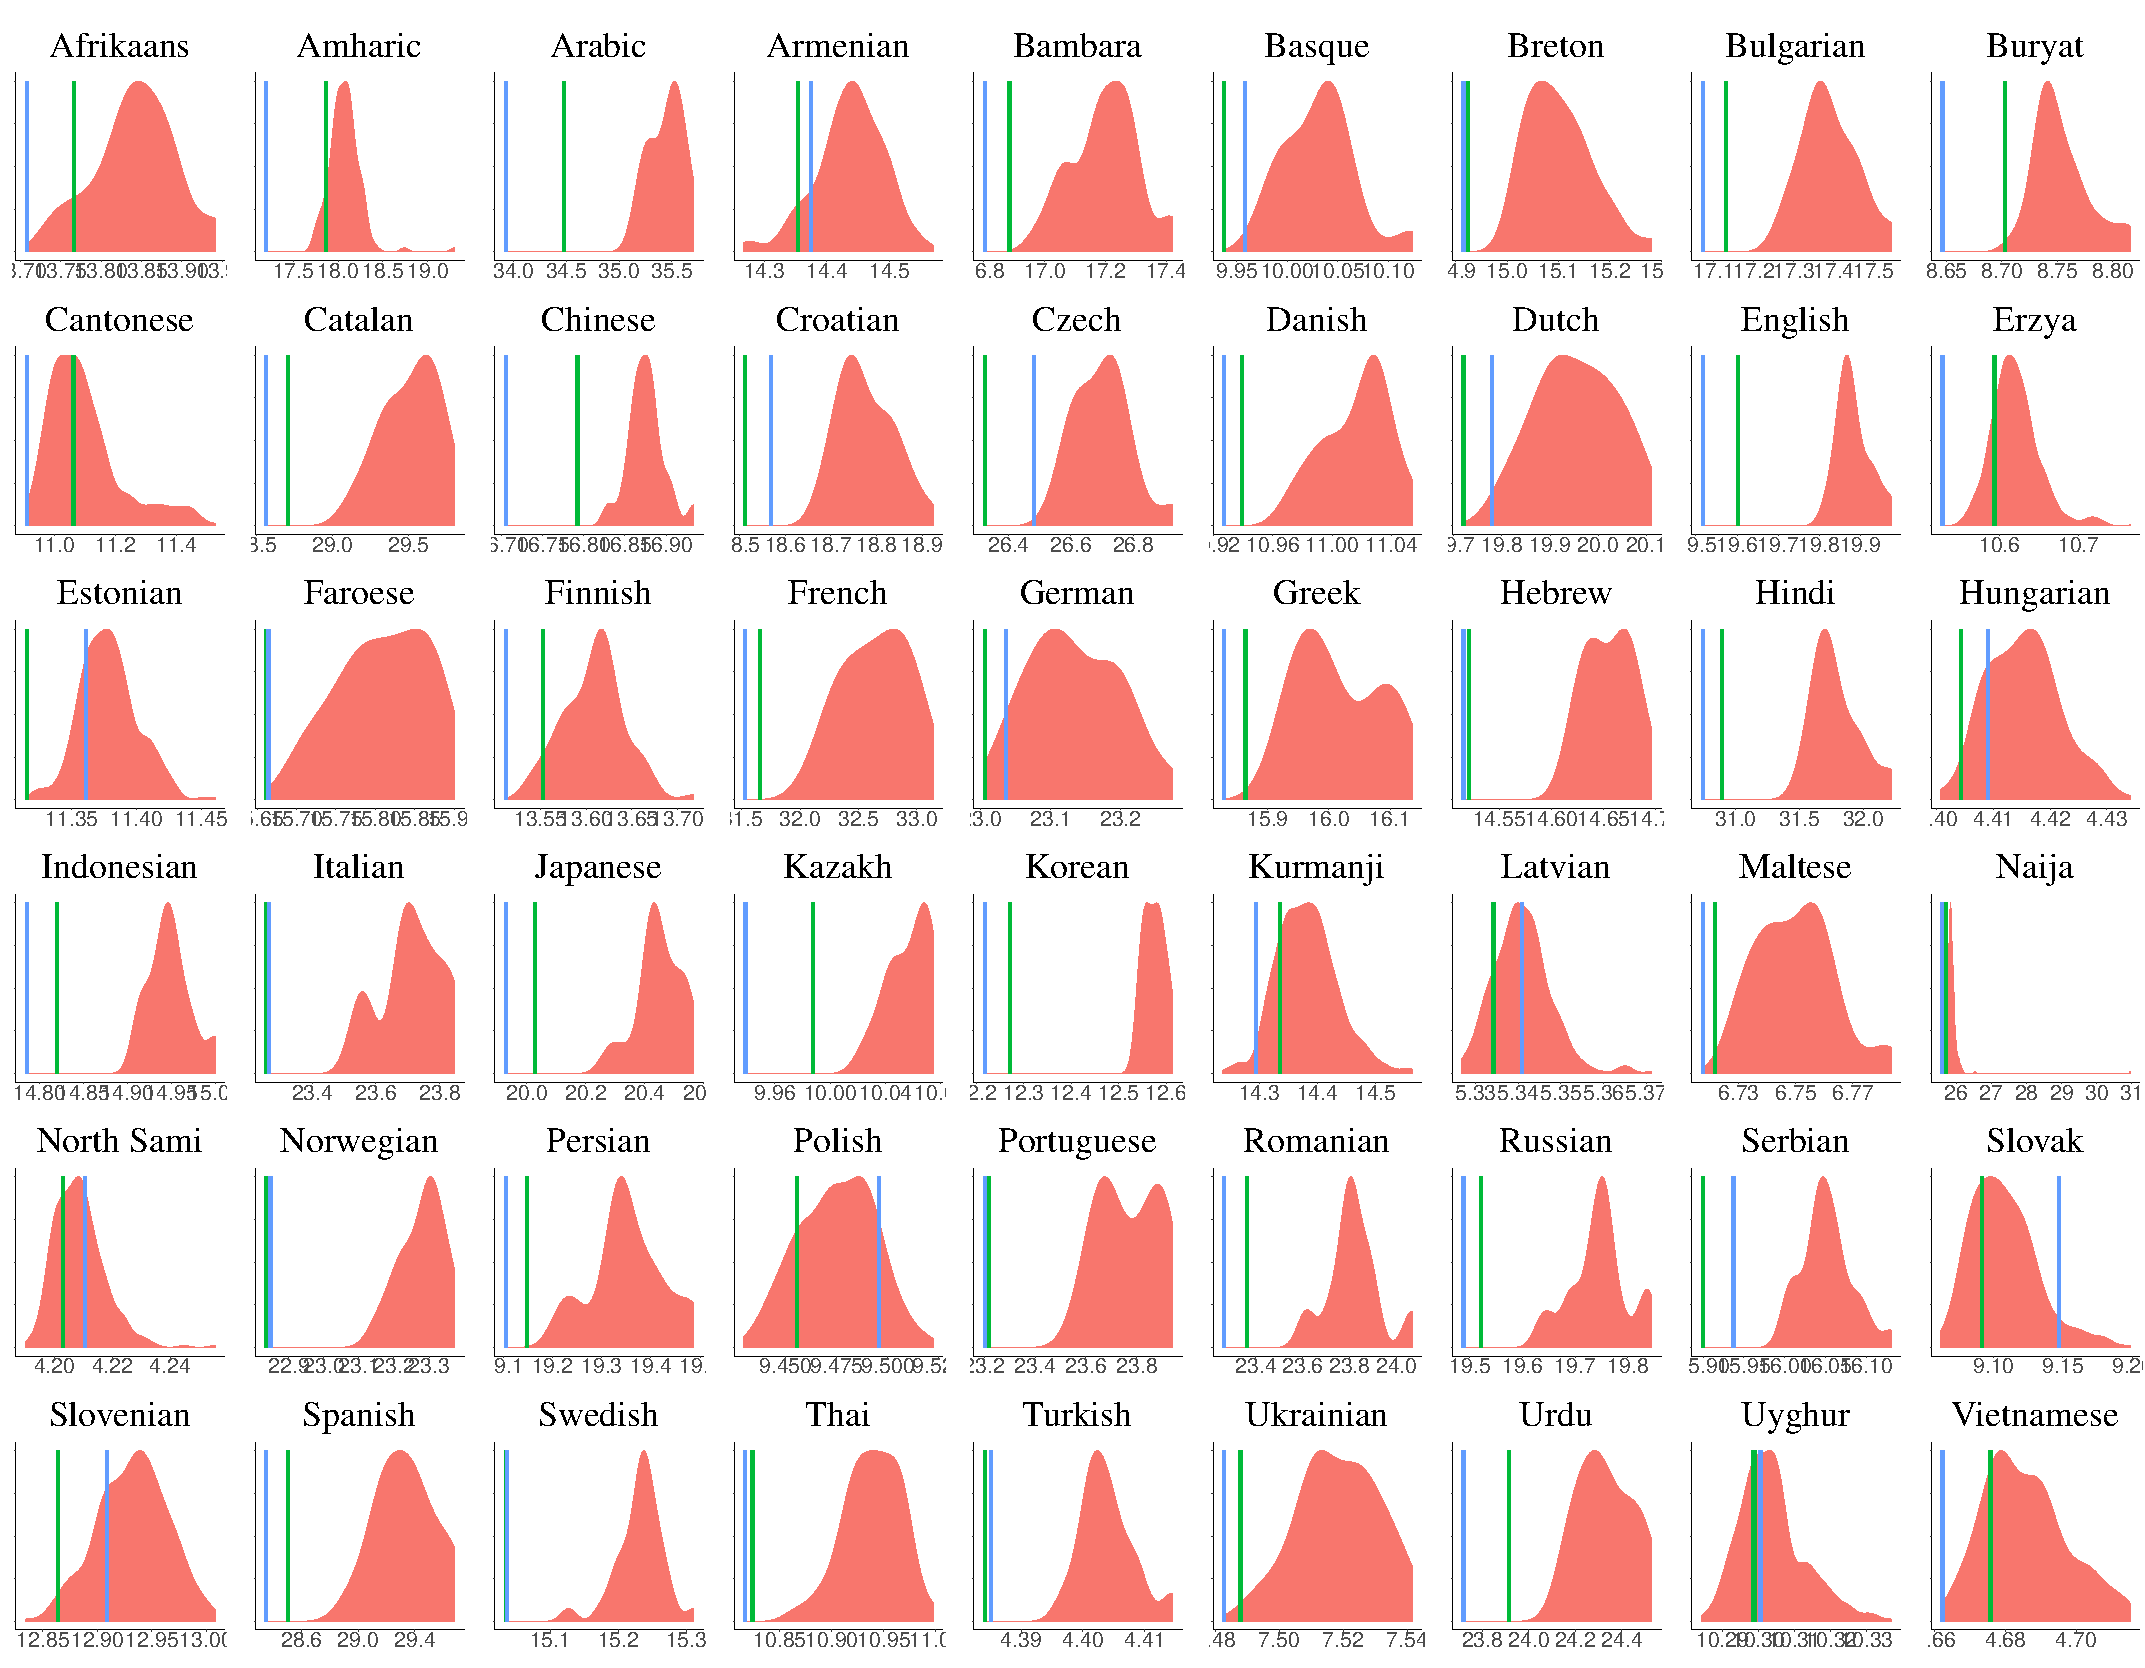
\includegraphics[width=\textwidth]{auc-table_MLE.pdf}
\end{center}
\caption{Histograms for the Area under the Curve (AUC) for the memory--surprisal tradeoffs for real (\mhahn{TODO color}) and random baseline (\mhahn{red}) orders, and for orders according to extracted grammars (\mhahn{TODO color}).
Compare Figure~\ref{fig:auc}. \mhahn{TODO make colors consistent with previous figure}
}\label{fig:auc-mle}
\end{figure}





%\begin{figure}
%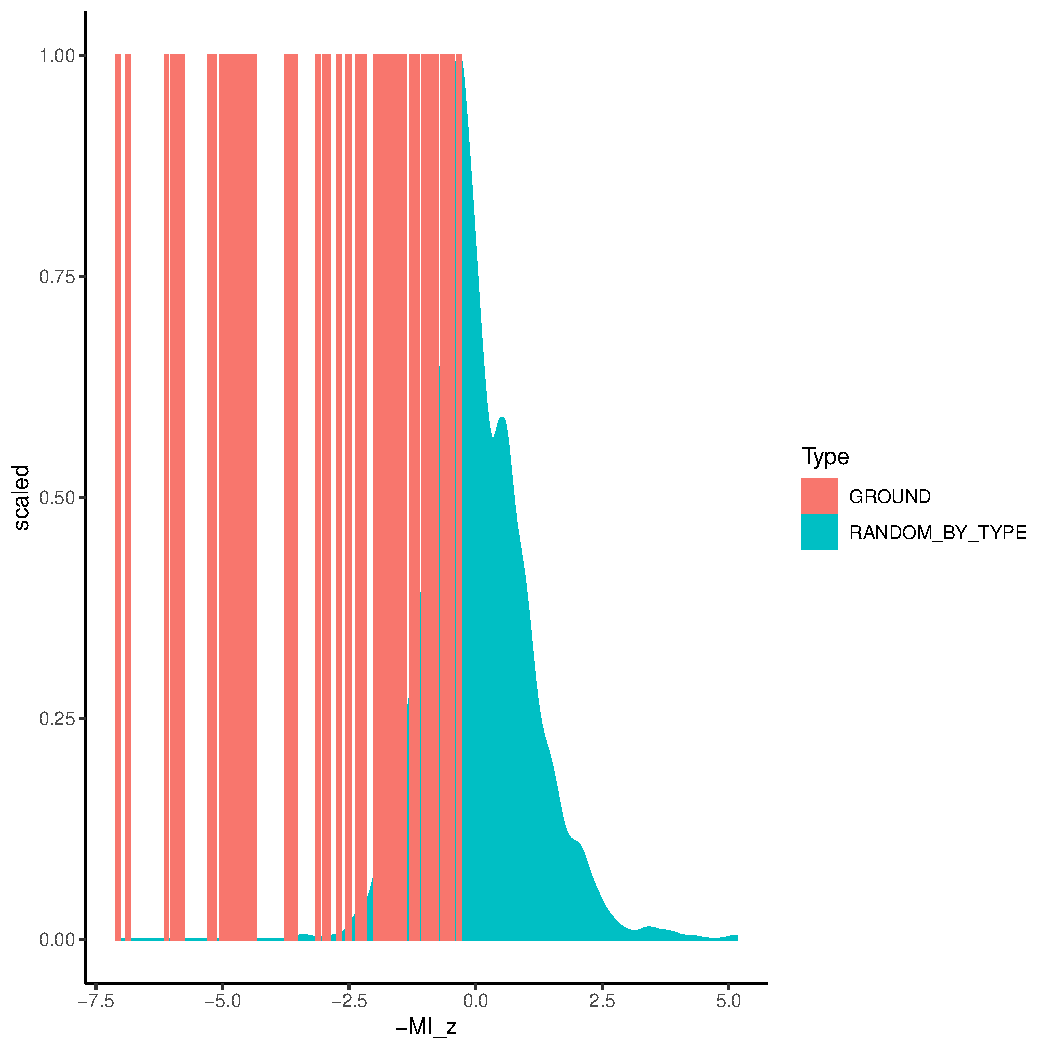
\includegraphics[width=0.5\textwidth]{figures/full-GROUND-listener-surprisal-memory-HIST_z_byMem_onlyWordForms_boundedVocab.pdf}
%	\caption{Histogram}\label{fig:hist-real}
%\end{figure}

\subsubsection{Taking Information Structure into Account}\label{sec:czech}

Languages with flexible word order often show a strong influence of information structure on word order \cite{givon1988pragmatics,jacobs1988probleme,neelemen2016word}.
Due to the difficulty of annotating information structure, only relatively few datasets have annotations for information structure, and even fewer datasets have both syntactic and information structure annotation.
We draw on the Prague Dependency Treebank of Czech \citep{bohmova2003prague,mikulova2006annotation}, which has both types of annotation.
Czech is a language with relatively high degree of word order freedom, which is generally thought to be strongly impacted by information structure \citep{firbas1966defining,firbas1974aspects}.

About one third of the Prague Dependency Treebank has annotation for topic-focus articulation \citep{mikulova2006annotation}.
Constituents are annotated for contrastiveness and for contextual boundedness, i.e., givenness.
Three labels are used:
``c'' for contrastive and contextually bound, ``f'' for contextually non-bound, ``t'' for non-contrastive contextually bound.
These labels are diagnosed based on constituent order and intonation.
Some constituents remain unmarked, the vast majority of these are function words such as adpositions, conjunctions, and auxiliaries; we introduce a label ``NA'' for these.
To define baselines, we extend the word order grammar formalism by defining separate weights for each combination of the 37 syntactic relations and these four information structure labels.

We obtained 38,727 training sentences and 5,228 dev sentences.

We created 20 baseline grammars with information structure, 20 baseline grammars without it, and created 5 model runs for both real orders and the fitted grammar.

\paragraph{Results}

We show estimated tradeoffs and the distributions over AUC values in Figure~\ref{fig:median-czech-infostruc}.
As this experiment was conducted only on the subset of the Prague Dependency Treebank that has information structure annotation, the numerical values are slightly different from those in Section \ref{sec:main-experiment-results}.

We compare the real orders both with the same baselines as above (red), and with the baselines taking information structure into account (green).
Baselines show a larger gap in efficiency between real and baseline grammars when the baselines condition word order on information structure.




In Figure~\ref{fig:freedom-mi-with-infostruc}, we provide a version of Figure~\ref{fig:freedom-surp} showing how the data point for Czech would move when modeling word order including information structure.
When modeling information structure, branching direction entropy decreases, while the surprisal difference between real and baseline orders increases.
This suggests that the weaker optimization in free word order languages observed in Experiment 2 might in part be because ordering grammars did not take information structure into account.
	
\paragraph{Discussion}
Using data from Czech, we found that the difference between the memory-surprisal tradeoffs of real and baseline orders increases if we choose baseline orderings that encode information structure, as real orders do.
We hypothesize that this in part explains why the strength of memory efficiency optimization in Section~\ref{sec:main-experiment-results} is negatively correlated with the degree of word order freedom:
Languages wit flexible word order typically encode information structure in word order, which increases average surprisal.
This does not mean that conditioning word order on information structure makes language less efficient in general.
Rather, encoding information structure in word order may increase the information content transmitted to the listener, which may in turn balance an increase in surprisal processing effort \citep{hahn2020universals}.
Due to the difficulty and cost of annotating information structure, we could only evaluate this hypothesis on data from one language.
As more annotated data becomes availabe, this should be replicated on data from further languages.

	


	
\begin{figure}
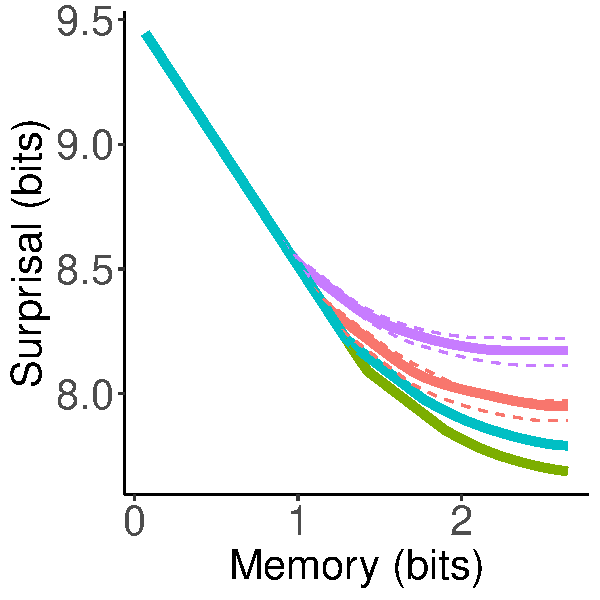
\includegraphics[width=0.5\textwidth]{figures/Czech-PDT-listener-surprisal-memory-MEDIANS_onlyWordForms_boundedVocab.pdf}
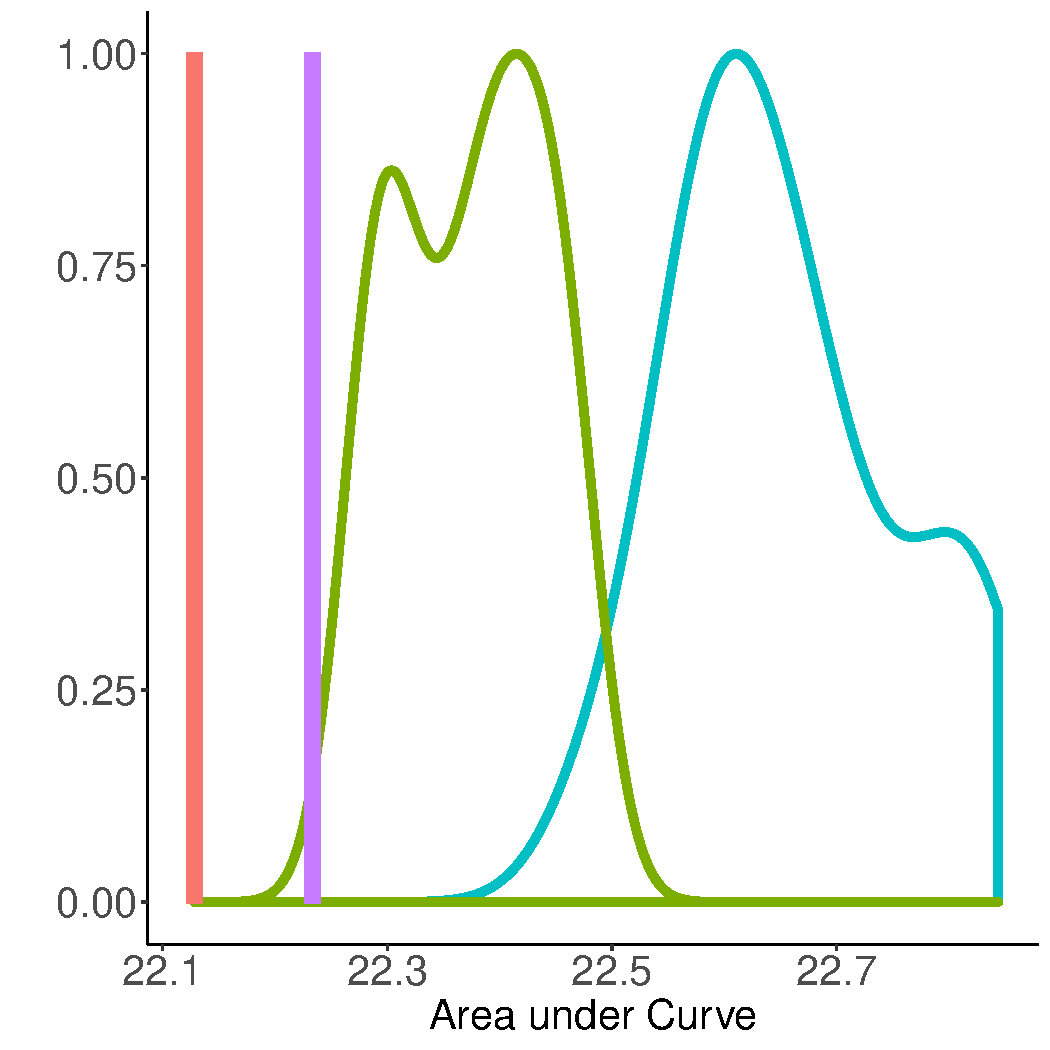
\includegraphics[width=0.5\textwidth]{figures/Czech-PDT-listener-surprisal-memory-HIST_AUC_onlyWordForms_boundedVocab_REAL-infostruc.pdf}

	\caption{Left: Memory-surprisal tradeoff Czech with information structure. Green: Baselines with information structure. Red: Baselines without information structure. Blue: Real. Right: AUC for Czech, for baselines without information structure (red) and baselines with information structure (green). Optimization of real orders is stronger when considering information structure in baselines. \mhahn{make colors and font size compatible}}\label{fig:median-czech-infostruc}
\end{figure}


	
\begin{figure}
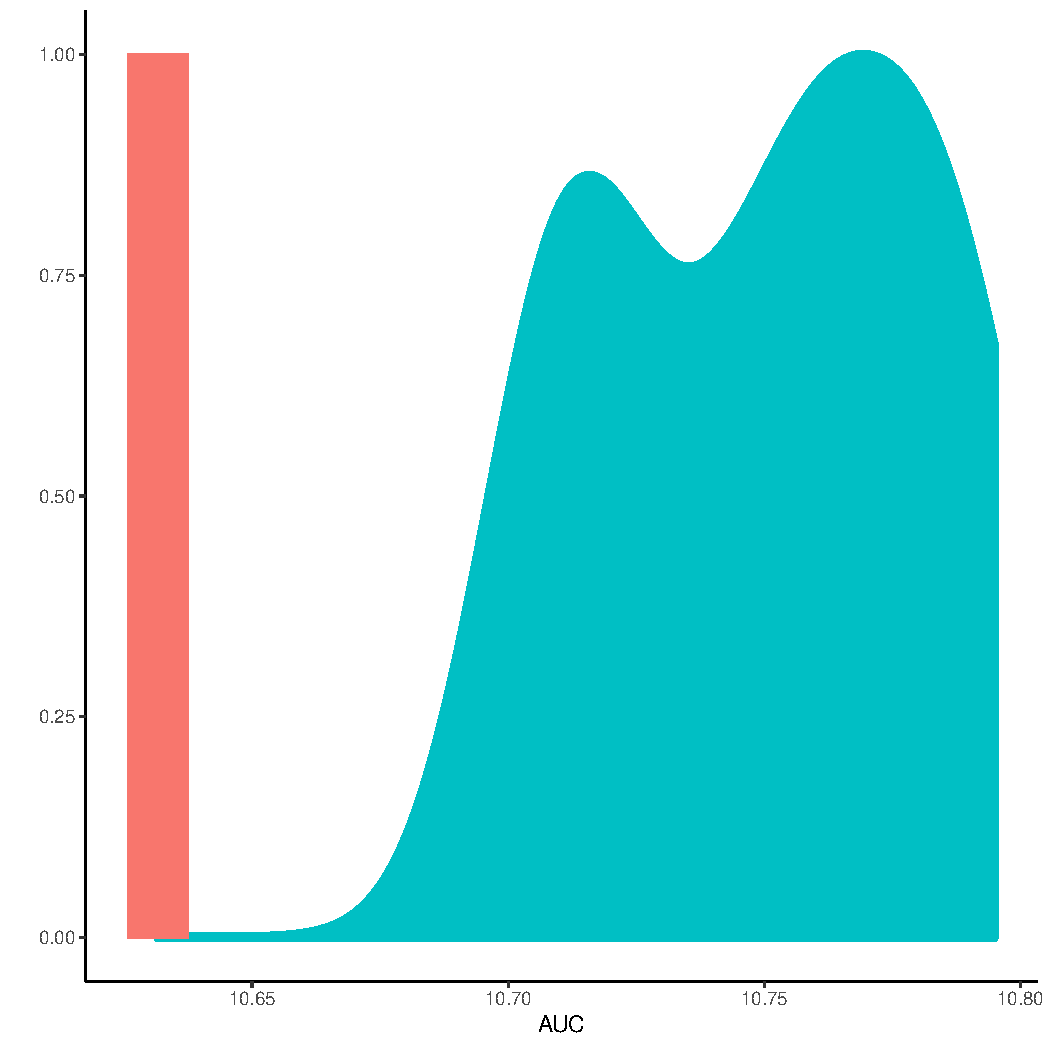
\includegraphics[width=0.5\textwidth]{writeup/figures/Czech-PDT-listener-surprisal-memory-HIST_AUC_onlyWordForms_boundedVocab_REAL-infostruc_GROUND.pdf}
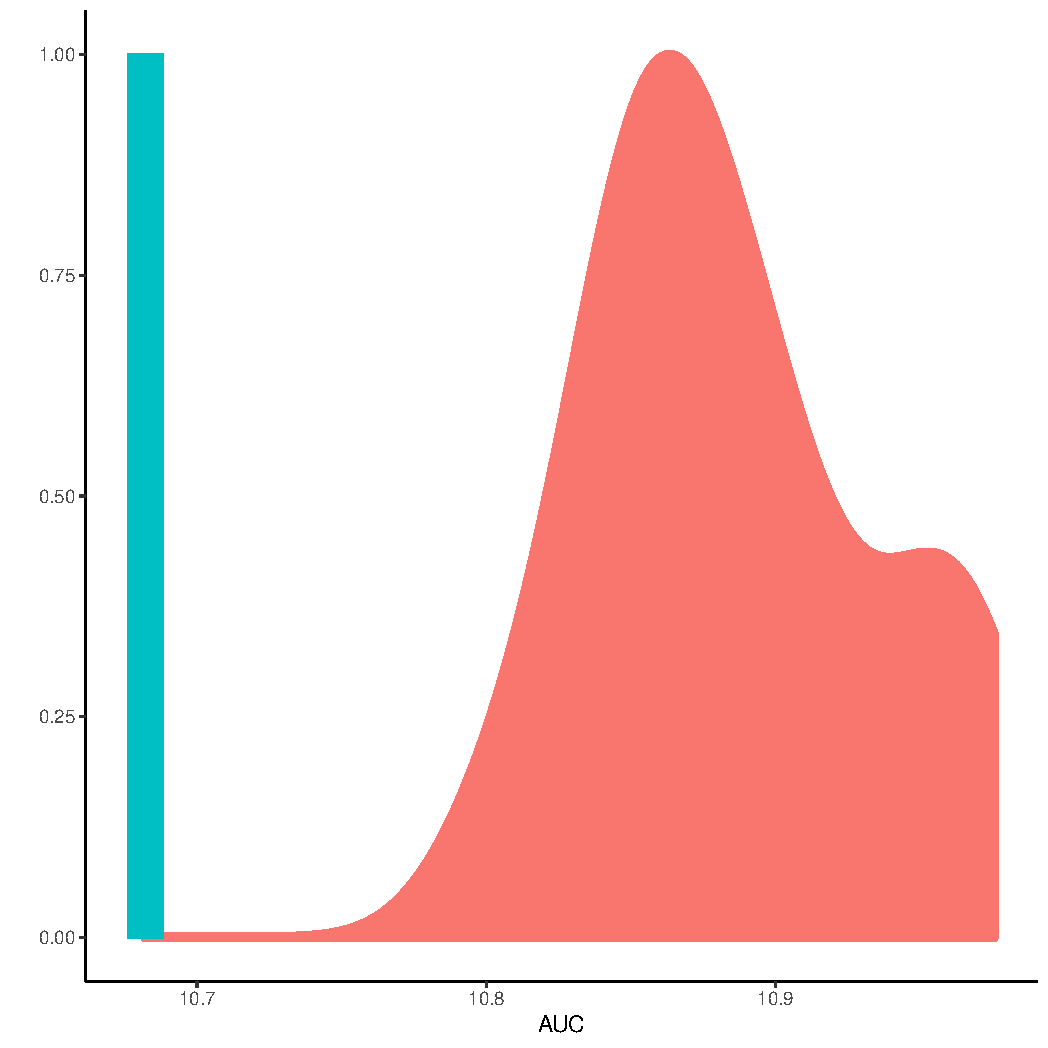
\includegraphics[width=0.5\textwidth]{writeup/figures/Czech-PDT-listener-surprisal-memory-HIST_AUC_onlyWordForms_boundedVocab_REAL-infostruc_REAL.pdf}

	\caption{\mhahn{TODO}}\label{fig:median-czech-infostruc}
\end{figure}





\begin{figure}
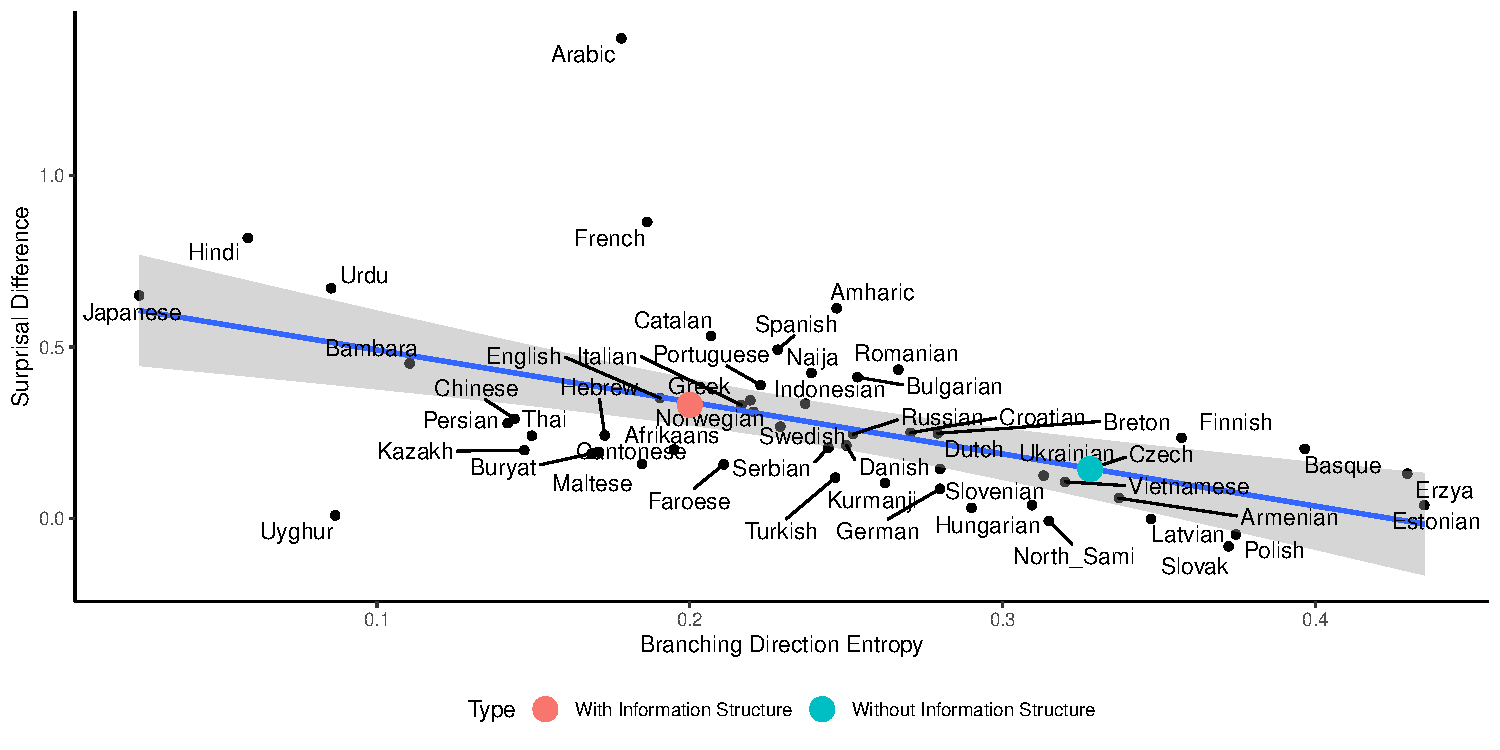
\includegraphics[width=0.9\textwidth]{figures/surprisal-branching-entropy-REAL-infostruc-invert.pdf}
	\caption{Order Freedom vs Difference in Surprisal at maximal memory (compare Figure~\ref{fig:freedom-surp}). The arrow indicates how the data point for Czech would move when modeling word order including information structure.
	When modeling information structure, branching direction entropy decreases, while the surprisal difference between real and baseline orders increases.
	This suggests that the weaker optimization in free word order languages observed in Experiment 2 might in part be because ordering grammars did not take information structure into account.
	}\label{fig:freedom-mi-with-infostruc}
\end{figure}




%
%\subsection{Discussion: Alternative Models}
%In view of the NLP literature, the following are the main other options that exist for estimating mutual information and probabilities in sequences:
%
%A traditional model uses n-gram models. A challenge of n-gram models is that they do not express any morphosyntactic generalizations. Furthermore, standard n-gram models do not express any generalizations about pairs of words that are not adjacent -- e.g., encoding a generalization about morphological agreement between two words is hard for such a model to capture if the two words are not always adjacent. Both the small scale of available corpora in many languages and free word order in many languages with rich morphology thus seem to make such models unattractive.
%We evaluate our hypothesis using n-gram models in SI Section X, confirming the conclusions obtained from neural models.
%
%A second option is to construct a statistical grammar, such as PCFG.
%The challenge is to encode statistical morphosyntactic generalizations, and to decide which independence assumptions to put into the model.
%One can either decide on a language-specific basis which generalizations to put in (laborious and might introduce bias), or choose a general model family that is rich enough to learn generalizations.
%The second option will make this a machine learning model that, for our purposes, does not seem to be superior to a recurrent neural network.
%



%\subsection{Data}
%\subsection{Setup}
%The recurrent neural network architecture has a range of adjustable parameters such as the number of neurons.
%For each language, we used Bayesian optimization using the Expected Improvement acquisition function (CITE) \citep{snoek-practical-2012} to find a good setting of the hyperparameters, taking average surprisal on random grammars as the objective.
%This biases the hyperparameters towards favoring counterfactual grammars.

%\subsection{Setup}




%\paragraph{Data}
%Given a sequence of input words $w_1, ..., w_n \in V$, the model 
%%
%\textbf{TODO I'm describing this in a lot of detail. Alternatively, we can say this is a standard NLP method and refer to the NLP literature for the definition.}
%The first component of such a model is an \emph{embedding matrix} $W_{emb} \in \mathbb{R}^{|V| \times d_{emb}}$, where the \emph{vocabulary} $\mathcal{V}$ is a set, containing the words that occur in the corpus, and $d_{emb} \in \mathbb{N}$ is a fixed parameter.
%This matrix assigns a $d_{emb}$-dimensional vector to each word occurring in the corpus.
%The second component is an LSTM cell $f_{LSTM}$, a nonlinear transformation mapping an \emph{input} vector $x_{i} \in \mathbb{R}^{d_{emb}}$ a \emph{hidden state} $h_i \in \mathbb{R}^{d_{LSTM}}$ and a \emph{cell state} $c_i \in \mathbb{R}^{d_{LSTM}}$ to a new pair of hidden state and cell states $h_{i+1}, c_{i+1} \in \mathbb{R}^{d_{LSTM}}$.
%The LSTM cell $f_{LSTM}$ is parameterized by a matrix of numerical parameters $W_{LSTM}$.
%
%%Such networks estimate the probability of a word in context as follows.
%Given a sequence of input words $w_1, ..., w_n \in V$, the model first retrieves fixed-dimensionality vector representations $x_1, ..., x_n$, where $x_i$ is the row of $W_{emb}$ corresponding to the word $w_i$.
%It then computes a sequence of hidden and cell states by the following recurrent computation:
%\begin{align*}
%	h_1, c_1 &:= 0 \\
%	h_2, c_2 &:= f_{LSTM}(x_1, h_1, c_1) \\
%	\dots \\
%	h_{n+1}, c_{n+1} &:= f_{LSTM}(x_n, h_n, c_n) \\
%\end{align*}
%The vector $h_i$ encodes the result of reading the words $w_1, ..., w_{i-1}$.
%We will write $LSTM(w_1, ..., w_{i-1})$ for $h_i$.
%
%The third component of the recurrent language model is the matrix $W_{output} \in \mathbb{R}^{|V| \times d_{LSTM}}$.
%We obtain per-word predictions of the next word by computing
%\begin{align*}
%	s_i := W_{output} h_i \in \mathbb{R}^{|V|} \\
%	p_i := \operatorname{softmax}(s_i)\in \mathbb{R}^{|V|} 
%\end{align*}
%where the softmax transformation normalizes vectors into probability distributions as follows
%\begin{equation}
%	\operatorname{softmax}(x)_i := \frac{\exp(x_i)}{\sum_{j=1}^{|V|} \exp(x_j)}
%\end{equation}
%Finally, the probability of the word $w_n$ in the context $w_1, ..., w_{n-1}$ is computed as
%\begin{equation}
%	p_\theta(w_n|w_1...w_{n-1}) := \frac{\exp((p_n)_{w_n})}{\sum_{w \in V} \exp(x_w)}
%\end{equation}
%and thus the surprisal is estimated as
%\begin{equation}
%- \log	p_\theta(w_n|w_1...w_{n-1}) := -\log \frac{\exp((p_n)_{w_n})}{\sum_{w \in V} \exp(x_w)}
%\end{equation}
%We discuss the choice of the numerical parameters in the next section.
%



%We collected data from the actual and random orderings in proportion one to two.
%The stopping criterion will be described below.

%Due to the randomness both in the sequence of training examples and the random initialization of the network weights, the results of the parameter estimation procedure will vary when run multiple times, especially on smaller datasets.
%Informally, due to the finiteness of the dataset, multiple parameter settings are compatible with the available training data.
%Consequently, memory-surprisal tradeoffs estimated on held-out sets will also show some variation.
%Therefore, we collect multiple samples for the actual orderings to control for variation due to the random initialization of the neural network.


%We chose these thresholds based on preliminary simulations which had suggested that these widths were achievable at acceptable computational cost.

%- at least 30 samples from both baseline and real
%
%- for the language-level tradeoff curve, either the fraction is zero or the bootstrapped CI has width $\leq 0.2$.



%
%(1) is bigram MI always greater in real languages?
%
%(2) is the tradeoff curve always lower than for deterministic simple grammar? for deterministic complex grammars? for stochastic simple/complex grammars?




%Training progresses in a series of parameter update steps, constructing updated parameters $\theta_0, \theta_1, \theta_2, \dots$.
%In the $n$-th update step, we first randomly select a word sequence $w_1 ... w_T$ from the training corpus, and use the LSTM using the current parameter setting $\theta_n$ to compute the per-word surprisals.
%We then update the parameter vector:
%\mhahn{maybe better to just say we use SGD}
%\begin{equation}\label{eq:train}
%	\theta_{n+1} := \theta_n + \alpha \partial_\theta \left(\sum_{i=1}^T \log p_\theta(w_i|w_1...w_{i-1})\right)
%\end{equation}
%where $\alpha \in \mathbb{R}_+$ is the \emph{learning rate}.



%We parameterized probabilistic ordering grammars as follows.
%For each relation type $\tau$, we introduce a \emph{direction parameter} $a_\tau \in [0,1]$ and a \emph{distance parameter} $b_\tau \in \mathbb{R}$.
%Each dependent is ordered on the left of its head with probability $a_\tau$ and to the right with probability $1-a_\tau$. 
%Then for each set of co-dependents $\{s_1, \dots , s_n\}$ placed on one side of a head, their order outward from the head is determined by iteratively sampling from the distribution $\operatorname{softmax}(b_{\tau_1}, \dots, b_{\tau_n})$ (\cite{goodfellow2016deep}, p. 184) without replacement. 
%Given a dependency tree, a probabilistic ordering grammar assigns a probability distribution over the possible projective linearizations of that tree.
%We use gradient descent to find parameters $a_\tau, b_\tau$ so as to maximize the overall likelihood of the orders in the actual corpus.
%We convert probabilistic ordering grammars into ordinary ordering grammars by the following method.
%Let $A_-$ be those relations $\tau$ where $a_\tau > 0.5$, similarly for $A_+$ those here $a_\tau \geq 0.5$.
%Then we order all relations in $A_-$ by $b_\tau$ in \emph{decreasing} order, and those in $A_+$ by $b_\tau$ in \emph{increasing} order.
%Then ordering a tree following the converted version is equivalent to greedily choosing the highest-probability linearization for the dependents of each head in a tree.
%We choose this method since maximum-likelihood grammars can be constructed with simple gradient descent.
%Another option would be to use some kind of discrete optimization method to approximate the original orders without a probabilistic method.
%However, discrete optimization is computationally challenging.


%Everything else is identical to Experiment 2.




%We test this hypothesis by comparing baseline languages to \emph{fixed-order} versions of the real languages.
%This enables us to tease apart the impact of the languages' word order rules from the impact of word order freedom.

%\mhahn{clean up text a bit}

%Above, we found that the majority of languages exhibit more favorable memory--surprisal trade-offs than counterfactual baselines based on random word order grammars. We also found that the strength of the difference between the real and baseline languages varies from language to language. Furthermore, we found that the magnitude of the difference is larger for languages with a higher degree of word order flexibility.




% Two issues: Confound because of restrictive formalism. 
% Association of efficiency and word order: By including information structure, we make the baselines worse
% Different orders based on info structure -> higher entropy when you don't have info structure

% Two controls:
% 1. Fixed-order baseline
% 2. Include info structure in the baseline, so that the baseline gets higher-entropy






\section{Study 3: Morpheme Order}\label{sec:morphemes}

%- datasets
%-- unimorph
%-- bibles corpus?
%-- celex
%- permute phonemes
%- permute syllables
%- permute phonemes only within syllables
%- permute morphemes 
%\section{Morphology}

\label{sec:morphemes}

The Efficient Tradeoff Hypothesis should apply not just at the level of words, but at the level of any linguistic element.
For instance, just as observed word orders exhibit information locality, the order of morphemes within words should also be structured so that morphemes which predict each other are close to each other.
Here, we apply the Efficient Tradeoff Hypothesis to predict the order of morphemes within morphologically complex words in two agglutinative languages. We study two agglutinative languages for which extensive corpora with hand-annotated morphological segmentation and labeling are available: Japanese and Sesotho. 
We compare the memory--surprisal tradeoff of the actual morpheme orders in these languages with hypothetical baseline orderings.
Furthermore, we construct hypothetical orderings that are optimized for the efficiency of the memory--surprisal tradeoff, and compare these to the actual morpheme orderings, to investigate whether morpheme order in these languages can be predicted by optimization of tradeoff efficiency.
Below, we first give brief sketches of the morphological patterns in these languages. 


\paragraph{Verb Suffixes in Japanese}

In Japanese, verbs are marked with an extensive number of suffixes. For example, the following verb forms are marked with multiple suffixes:

\ex.\ag. mi  rare mash yoo \\
%Stem (3) (5) (8) \\
see  \textsc{passive}  \textsc{politeness}  \textsc{future} \\
`will be seen'
\bg. mi taku nakat ta \\
%Stem (6) (7) (8) \\
see \textsc{desiderative} \textsc{negation} \textsc{past} \\
`did not wish to see'

Based on corpus data and the linguistic literature on Japanese, we identified the following frequent verb suffixes, occurring in the following order outwards from the verb root (see SI for details).


\begin{enumerate}
\item \textit{suru}: obligatory suffix after Sino-Japanese words when they are used as verbs
\item Valence: causative (-\textit{ase}-) (\citet[142]{hasegawa2014japanese}, \citet[Chapter 13]{kaiser2013japanese})
\item Voice and Mood: passive (-\textit{are}-, -\textit{rare}-) (\citet[152]{hasegawa2014japanese}, \citet[Chapter 12]{kaiser2013japanese}) and potential (-\textit{e}-, -\textit{are}-, -\textit{rare}-) \citep[398]{kaiser2013japanese}  
\item Politeness (-\textit{mas}-) \citep[190]{kaiser2013japanese}.
\item Mood: desiderative (-\textit{ta}-) \citep[238]{kaiser2013japanese}
\item Negation (-\textit{n}-)
\item Tense, Aspect, Mood, and Finiteness: past (-\textit{ta}), future/hortative (-\textit{yoo}) \citep[229]{kaiser2013japanese}, nonfiniteness (-\textit{te}) \citep[186]{kaiser2013japanese}
%\item Nonfiniteness: the suffix -\textit{te} derives a nonfinite form .
\end{enumerate}

%In accordance with Bybee's hierarchy, valence is marked closest to the verb, followed by voice.
%Unlike predicted by the hierarchy, tense/aspect markers are not placed closer to the verb than mood/modality markers.






\paragraph{Verb Affixes in Sesotho}
Sesotho (also known as Southern Sotho) is a Southern Bantu language spoken primarily in Lesotho and South Africa.
Sesotho verbs are marked with both prefixes and suffixes \citep{demuth1992acquisition}.
Common prefixes include markers for agreement with subjects and objects; object prefixes always follow subject prefixes \ref{ex:oadireka}.
Common suffixes include markers changing valence and voice, and a mood suffix \ref{ex:ophehela}.

\ex.\ag. oa di rek a \\
\textsc{subject.agreement} \textsc{object.agreement} buy \textsc{indicative} \\
`(he) is buying (it)'  \citep{demuth1992acquisition} \label{ex:oadireka}
\bg. o pheh el a \\
\textsc{subject.agreement} cook \textsc{applicative} \textsc{indicative} \\
`(he) cooks (food) for (him)'  \citep{demuth1992acquisition}
\label{ex:ophehela}

We identified affix morphemes and their ordering based on the analysis in \cite{demuth1992acquisition}, supplemented with information from grammars of Sesotho \citep{doke1967textbook,guma1971outline}. See SI for details.
We identified the following prefixes:

\begin{enumerate}
    \item Subject agreement: This morpheme encodes agreement with the subject, for person, number, and noun class (the latter only in the 3rd person) \cite[\textsection 395]{doke1967textbook}.
	    The annotation provided by \cite{demuth1992acquisition} distinguishes between ordinary subject agreement prefixes and agreement prefixes used in relative clauses; we distinguish these morpheme types here.
    
    \item Negation \citep[\textsection 429]{doke1967textbook}
    
    \item Tense/aspect marker   \citep[\textsection 400--424]{doke1967textbook}
    
    \item Object agreement or reflexive marker \citep[\textsection 459]{doke1967textbook}. 
    Similar to subject agreement, object agreement denotes person, number, and noun class features of the object.
\end{enumerate}
We identified the following suffixes:

% something we might cite at some point (pointers from Beth Levine), about templatic morpheme order in Bantu
% Hyman2003 in literature.bib
% Jeffrey Good, Strong Linearity: Three Case Studies Towards a Theory of Morphosyntactic Templatic Constructions (Diss, 2003)
    
\begin{enumerate}
\item Semantic derivation: reversive (e.g., `do' $\rightarrow$ `undo') \citep[\textsection 345]{doke1967textbook}
\item Valence: Common valence-altering suffixes include causative, neuter/stative, applicative, and reciprocal \citep[\textsection 307--338]{doke1967textbook}. See SI for details on their meanings.
    \item Voice: passive \citep[\textsection 300]{doke1967textbook} 
    \item Tense \citep[\textsection 369]{doke1967textbook}
    \item Mood \citep[\textsection 386--445]{doke1967textbook}
    \item Interrogative and relative markers, appended to verbs in certain interrogative and relative clauses \citep[\textsection 160, 271, 320, 714, 793]{doke1967textbook}.
    %-\textit{ng}.
    %The interrogative marker -\textit{ng} is an enclitized form of the interrogative `what'.
    %The relative marker -\textit{ng} is suffixed to verbs in relative clauses.
\end{enumerate}



%For prefixes, in agreement with Bybee's hierarchy, subject agreement is encoded in a position further away than TAM features.
%For suffixes, relation to Bybee hierarchy: valence closest, then voice, then tense, then mood.


\subsection{Experiment}
\paragraph{Data Selection and Processing}
For Japanese, we drew on Universal Dependencies data.
In the tokenization scheme used for Japanese, most affixes are separated as individual tokens, effectively providing morpheme segmentations.
We used the GSD corpus, Version 2.4, \citep{tanaka2016universal, asahara2018universal}, as it was the only corpus with a training set and freely available word forms.
In the corpus, verb suffixes largely correspond to auxiliaries (with tag \texttt{AUX}); only a few morphemes tagged \texttt{AUX} are not standardly treated as suffixes (see SI), and one frequent suffix (-\textit{te}) is labeled \texttt{SCONJ}.
We selected verb forms by selecting all chains of a verb (tag \texttt{VERB}) followed by any number of auxiliaries (tag \texttt{AUX}) from the training set of the corpus. When the suffix -\textit{te} (tag \texttt{SCONJ}) followed such a chain, we added this.
We labeled suffixes for underlying morphemes with the help of the lemmatization provided for each suffix in the corpus (see SI Section 4.3 for details).
The passive and potential (slot 3) markers are formally indistinguishable for many verbs.
As we cannot systematically distinguish them on the basis of the available corpus annotation, we merge these into a single underlying morpheme `Passive/Potential'.

We obtained 15,281 verb forms in the training set and 1,048 verb forms in the held-out set.
Of the forms in the training set, 27\% had two or more suffixes (modal group: two suffixes, accounting for 20\% of forms; maximum seven suffixes).
While predicting order naturally focuses on datapoints with more than one suffix, we include the other datapoints for estimating conditional mutual information $I_t$.
%We used the annotation provided in the corpus to identify underlying morphemes (see SI).

%In the corpus, each morpheme is annotated with a lemma, indicating a normalized context-independent representation of the morpheme.
%For both verbs and affixes, this lemma annotation abstracts away from most morphophonological and other allomorphic variation, it thus largely identifies underlying morphemes (see SI for limitations).

For Sesotho, we used the Demuth Corpus \citep{demuth1992acquisition} of child and child-directed speech, containing about 13K utterances with 500K morphemes.
The corpus has very extensive manual morphological segmentation and annotation; each verb form is segmented into morphemes, which are annotated for their function.
Sesotho verbs carry both prefixes and suffixes.
We extracted 37K verb forms (see SI 4.2 for details).
We randomly selected 5\% to serve as held-out data and used the remaining 95\% as training data.
93\% of forms had two or more affixes (modal group: three affixes, accounting for 36\% of forms; maximum eight affixes).


\paragraph{Estimating Memory-Surprisal Tradeoff}
We modeled incremental prediction on the level of morpheme sequences.
To do so, we represented each verb form as a sequence of a stem and affix morphemes, abstracting away from morphophonemic interactions between neighboring morphemes.
As in many languages, affixes in Japanese and Sesotho show morphophonemic interactions between neighboring morphemes; for instance, the Japanese politeness morpheme -\textit{mas}- takes the form -\textit{masu} when it is word-final, while it has the allomorph -\textit{mase}- when followed by the negation suffix -\textit{n}.
Modeling prediction on the level of morphemes, as opposed to phonemes, controls for these interactions.\footnote{See SI Section 4.3 for qualitatively similar results when modeling prediction at the phoneme level.}

In analogy to Studies 1--2, we modeled verb forms as a stationary stochastic process by concatenating the verb forms from the corpus in random order.

We calculated $I_t$ by estimating an $n$-gram model on the training set and then computing the average surprisal $S_t$ as cross-entropy on the held-out set using Kneser-Ney smoothing.
The model may overfit as the context size $t$ increases, leading to higher cross-entropies for larger values of $t$.
We mitigated overfitting for large $t$ by estimating
\begin{equation}
\hat{S}_t := \min_{s \leq t} S_s,
\end{equation}
where $S_s$ is the cross-entropy of the $s$'th order Markov model on held-out data.
This procedure ensures that $\hat{S}_t$ can only decrease as the context size $t$ increases.
Similar results were obtained when instead using the simple `naive' estimator for $I_t$ on the training set; this naive estimator estimates $I_t$ directly from $n$-gram counts in the training set; see the SI for details.

\paragraph{Parameterizing Alternative Orderings}

We parameterized alternative affix orderings by assigning a weight in $[0,1]$ to each morpheme.
Given such a grammar, affixes are ordered by the values assigned to their underlying morphemes.
We considered all morphemes annotated in the corpora, including low-frequency ones going beyond the ones identified above (see SI for details).


To verify that this formalism is appropriate for capturing morpheme order in Japanese and Sesotho, we fitted models parameterized in this way to the observed orders.
Ordering morphemes according to these fitted models recovered the observed order for almost all forms (98.6 \% for Japanese, 99.93\% for Sesotho prefixes, 97.4\% for Sesotho suffixes). Exceptions largely concern low-frequency affixes beyond those considered here. We take this as confirmation that the formalism is generally suited to capture morpheme order.


\paragraph{Creating Optimal Orders}

In order to create optimal orders to compare real orders to, we optimized orderings for the AUC under the memory--surprisal tradeoff curve with an adaptation of the hill climbing method that \citet{gildea-human-2015} used to optimize word order grammars for the length of syntactic dependencies and trigram surprisal.

We randomly initialized the assignment of weights to morphemes, and then iteratively change the assignment to reduce AUC.
In each iteration, we randomly chose one morpheme, and evaluate AUC for each way of ordering it between two other morphemes.
We then updated the weights to the ordering that yields the lowest AUC.
To speed up optimization, we restricted to morphemes occurring at least 10 times in the corpus for 95\% of iterations, and to 10\% of possible orderings in each step.
These choices vastly reduced computation time by reducing time spent on low-frequency morphemes.
This optimization method is approximate, as it only guarantees convergence to a local optimum \citep{gildea-human-2015}, not to a globally optimal assignment.

We ran this method for 1,000 iterations. Empirically, AUC converged after a few hundred iterations.
To control for the randomness in initialization and the optimization steps, we ran this algorithm ten times.
For Sesotho, we ran the algorithm separately for prefixes and suffixes due to computational efficiency considerations.\footnote{With the exception of the tense/aspect markers, none of the morpheme types discussed above can occur both as prefixes and suffixes. Therefore, we do not expect this separation to impact results.}

\subsection{Results}
In Figure~\ref{fig:morph-auc}, we compare the area under curve of the memory--surprisal tradeoff for Japanese and Sesotho verb forms under different orderings.
Both observed orders and the approximately optimized grammars show lower AUCs than all random baseline samples.
For comparison, we also show AUC for the order resulting from \emph{reversing} all suffix chains in the observed orders; this results in high AUC even exceeding most random grammars.
These results show that Japanese and Sesotho affix orderings enable approximately optimal memory--surprisal tradeoffs.



\begin{figure}
	\begin{center}
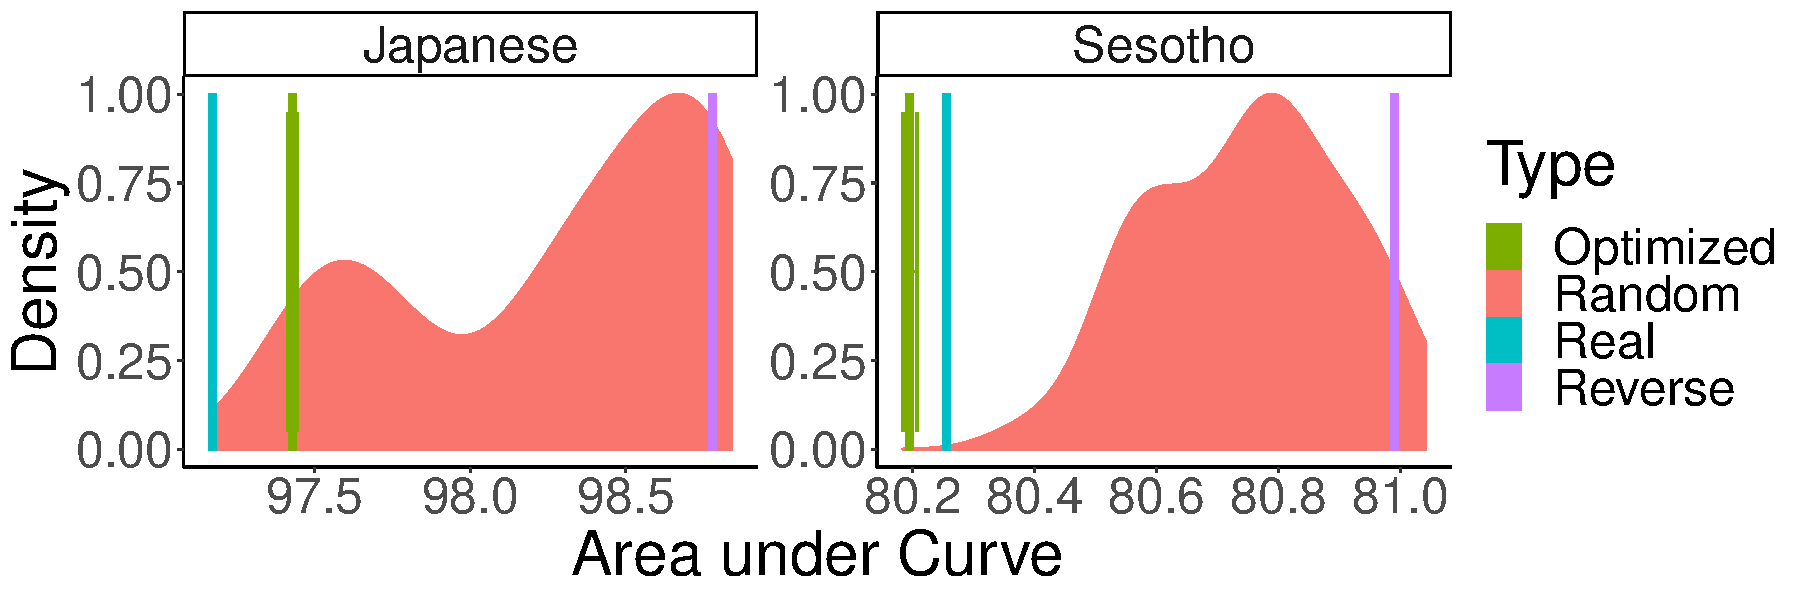
\includegraphics[width=\textwidth]{figures/Both-suffixes-byMorphemes-auc-hist-heldout.pdf}
\end{center}
	\caption{Areas under the curve for the memory--surprisal tradeoff for verb affixes in Japanese (left) and Sesotho (right). For the baseline grammars, we show a Kernel Density estimate.
	For the approximately optimized grammars, we show the mean AUC, with error bars ranging from minimal to maximal AUC among the ten grammars (almost imperceptible in Sesotho).
	In both Japanese and Sesotho, the AUC of the real orderings falls in the range of approximately optimized grammars.}
	\label{fig:morph-auc}
\end{figure}



%\begin{figure}
%	\begin{center}
%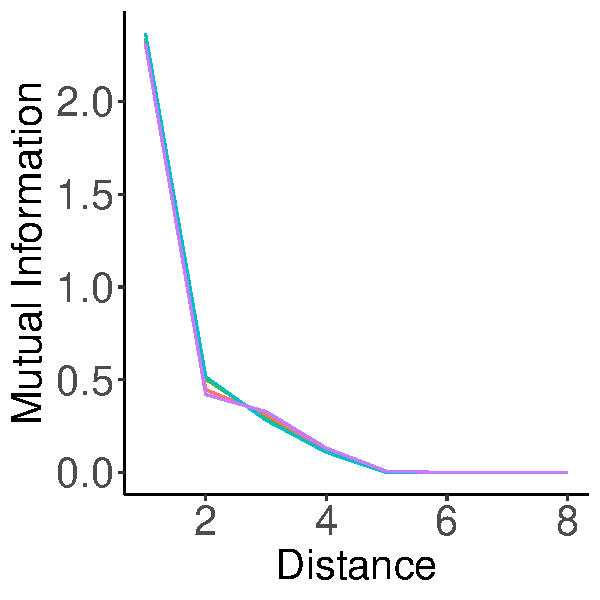
\includegraphics[width=0.3\textwidth]{figures/Japanese-suffixes-byPhonemes-it-heldout.pdf}
%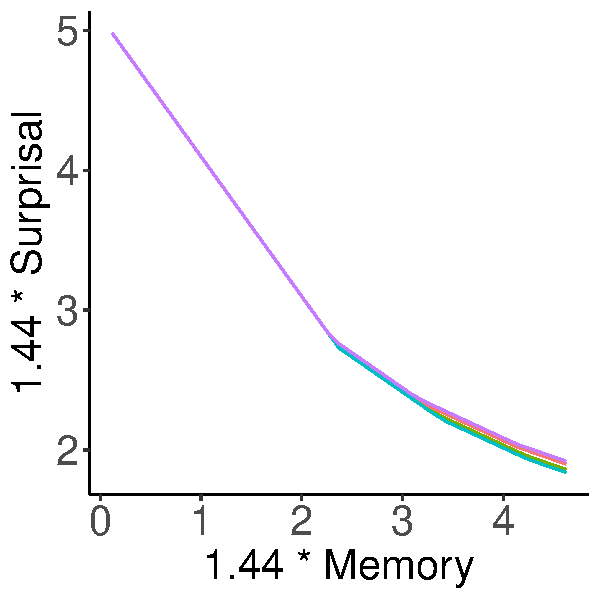
\includegraphics[width=0.3\textwidth]{figures/Japanese-suffixes-byPhonemes-memsurp-heldout.pdf}
%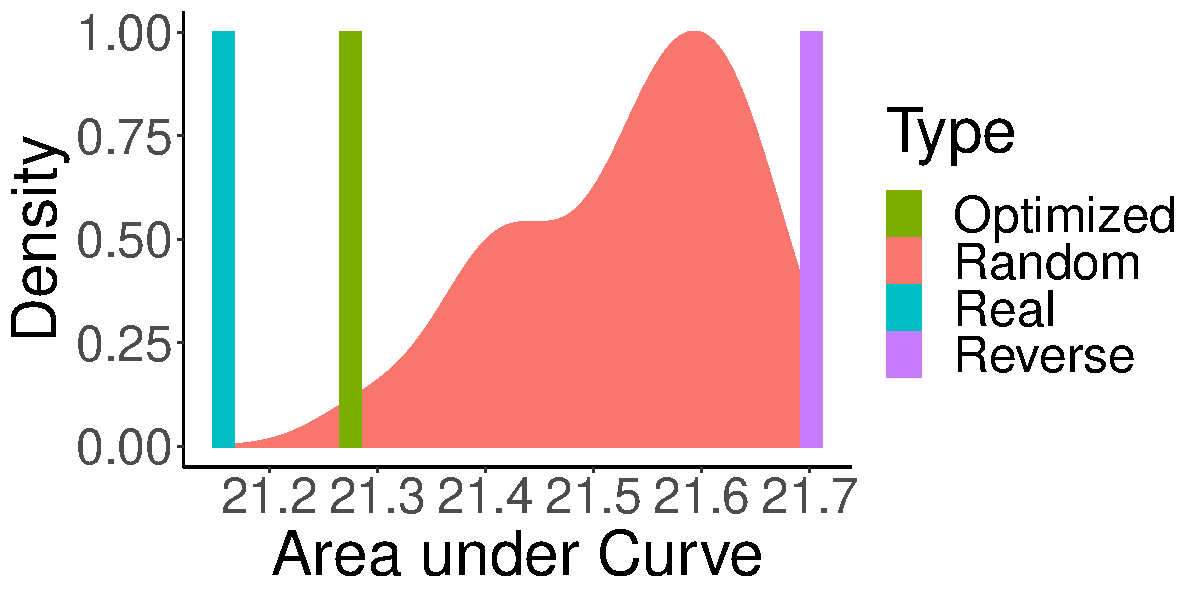
\includegraphics[width=0.3\textwidth]{figures/Japanese-suffixes-byPhonemes-auc-hist-heldout.pdf}
%
%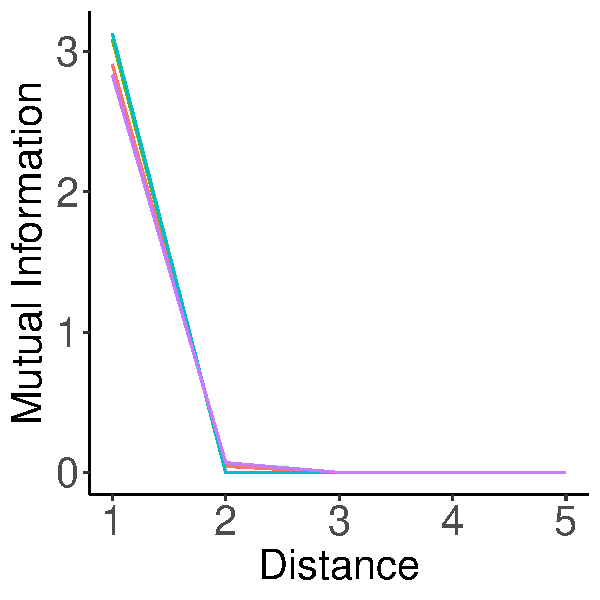
\includegraphics[width=0.3\textwidth]{figures/Japanese-suffixes-byMorphemes-it-heldout.pdf}
%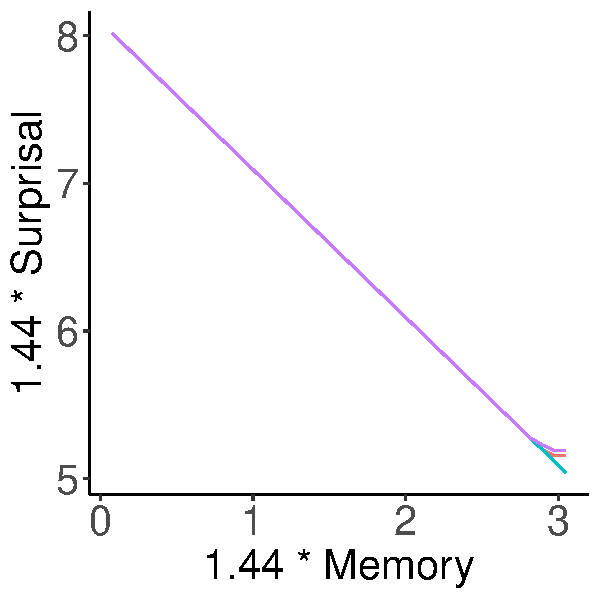
\includegraphics[width=0.3\textwidth]{figures/Japanese-suffixes-byMorphemes-memsurp-heldout.pdf}
%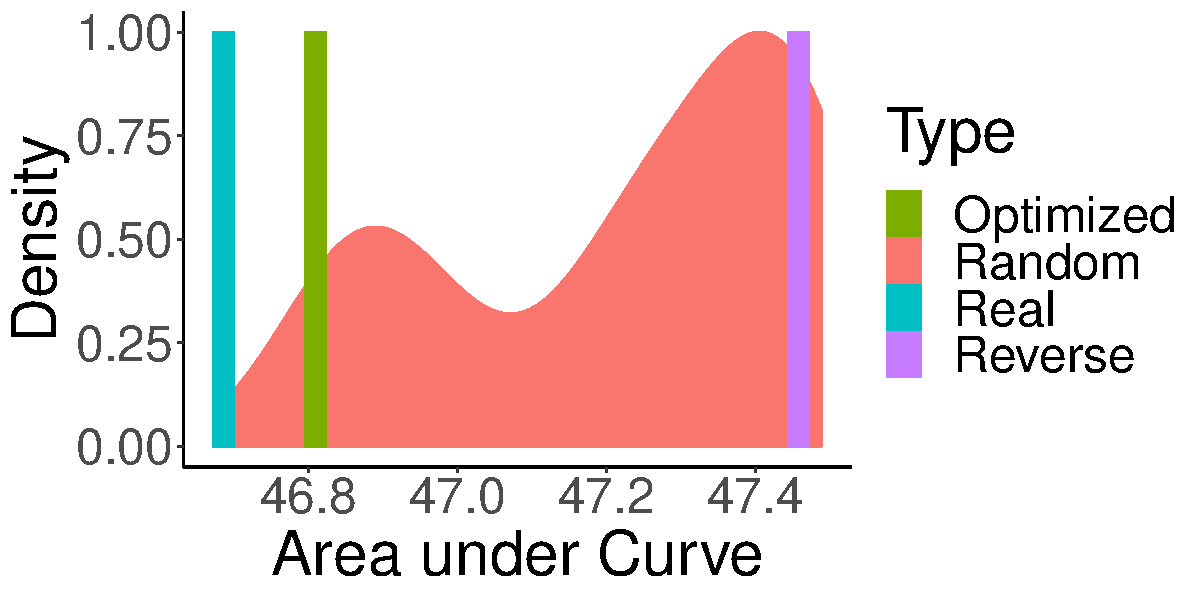
\includegraphics[width=0.3\textwidth]{figures/Japanese-suffixes-byMorphemes-auc-hist-heldout.pdf}
%\end{center}
%	\caption{Areas under the memory--surprisal tradeoff curve for Japanese verb suffixes.}\label{fig:jap-phon-morph}
	%\caption{Japanese verb suffixes, measuring prediction on the level of phonemes (top) and morphemes (bottom), for real (blue), random (green), and approximately optimized (red) orderings. Left: $I_t$ as a function of $t$. Center: Memory-surprisal tradeoff. Right: Areas under the curve for the memory--surprisal tradeoff.}\label{fig:jap-phon-morph}
%\end{figure}


We now ask to what extent the observed morpheme ordering is predicted correctly by approximately optimized grammars.
In Table~\ref{tab:morph-acc}, we give summary statistics about the accuracy of optimized grammars in predicting affix order in the corpus, together with random baseline figures.
We evaluate accuracy using two methods:
In one method (`Pairs'), we consider, for each verb form in the corpus, all pairs of prefixes (or suffixes).
We report the proportion of these pairs in the corpus for which the relative order of the two affixes is as predicted by the grammar.
In the other method, (`Full'), we report the proportion of verb forms in the corpus that has exactly the affix ordering predicted by the grammar.
In both measures, we average over all ten approximately optimized grammars for each language.

\begin{table}
\begin{tabular}{cc||ll|ll}
             &              & \multicolumn{2}{c}{Prefixes}    & \multicolumn{2}{|c}{Suffixes} \\
             &              & Pairs & Full & Pairs & Full \\ \hline\hline
Japanese    & Optimized   & -- &  -- &   0.953 (SD 0.011) & 0.943 (SD 0.014) \\ % updated
             & Baseline    & -- & --  & 0.497 (SD 0.287) & 0.425 (SD 0.29) \\ \hline % updated
Sesotho &   Optimized  &  0.988 (SD 0.0) & 0.989 (SD 0.0) & 0.756 (SD 0.014) & 0.676 (SD 0.017) \\
&   Baseline  &  0.672 (SD 0.305) & 0.604 (SD 0.338) & 0.423 (SD 0.204) & 0.332 (SD 0.211) \\ 
\end{tabular}
\caption{Accuracy of approximately optimized orderings, and of random baseline orderings, in predicting verb affix order in Japanese and Sesotho. `Pairs' denotes the rate of pairs of morphemes that are ordered correctly, and `Full' denotes the rate of verb forms where order is predicted entirely correctly. We show means and standard deviations over ten different runs of the optimization algorithm (`Optimized'), and over different random orderings (`Random').}\label{tab:morph-acc}
\end{table}

\paragraph{Japanese results.} In Japanese, by both measures, optimized grammars recover the observed orders with high accuracy.
We compare the real grammar with the approximately optimized grammar that achieved the lowest AUC value in Table~\ref{tab:grammar-table-jap}; the main divergence is that desiderative suffixes are placed after the negation suffix (slot 6), whereas real Japanese orders place them before the politeness suffix (slot 5).
We conducted an error analysis comparing the real Japanese morpheme order against our approximately optimized orders.
We extracted the pairs of morphemes whose relative order is incorrectly predicted, excluding pairs involving low-frequency morphemes not discussed here. 
Results are shown in Table~\ref{tab:jap-err-analysis}.
The most frequent divergence for this grammar is that politeness and negation suffixes are consistently ordered incorrectly; this affects 74 corpus examples (out of 15K total examples).

We also found that prediction was more accurate when modeling on the level of phonemes, suggesting that divergence between model predictions and actual order might be related to phonological pressure (see SI Section 4.3).

\begin{table} % updated forWords_Japanese_OptimizeOrder_MorphemeGrammar_Normalized_FullData_HeldoutClip/optimized_forWords_Japanese_OptimizeOrder_MorphemeGrammar_Normalized_FullData_HeldoutClip.py
    \centering
    \begin{tabular}{llllllll}
	    &	    Real & Optimized \\ \hline\hline
	    &    Stem & Stem \\ \hline
1 & suru & suru \\
2 & causative & causative \\
3 & passive/potential & passive/potential \\
4 & desiderative & negation \\
5 & politeness & future \\
6 & negation & politeness \\
7 & future & desiderative \\
 & past & nonfinite \\
 & nonfinite & past \\
 \hline
    \end{tabular}
    \caption{Comparing order of Japanese affixes in the observed orders (left) and according to an approximately optimized grammar (right). We organize the affixes in the real order into the seven slots described above.}
    \label{tab:grammar-table-jap}
\end{table}

\begin{table} % updated forWords_Japanese_OptimizeOrder_MorphemeGrammar_Normalized_FullData_HeldoutClip/optimized_forWords_Japanese_OptimizeOrder_MorphemeGrammar_Normalized_FullData_HeldoutClip.py
    \centering
    \begin{tabular}{ll|ll}
    \multicolumn{2}{c|}{Error} & Frequency \\ \hline\hline
politeness & negation & 74 \\
desiderative & negation & 14 \\
politeness & future & 9 \\
\end{tabular}
    \caption{Errors in Japanese: We show pairs of morphemes that are ordered incorrectly by the approximately optimized grammar with the lowest AUC value.
    We indicate the number of such pairs occurring in the corpus.
    We only show errors where both morphemes are among the high-frequency ones studied here.
    }
    \label{tab:jap-err-analysis}
\end{table}

\paragraph{Sesotho results.} We compare the real Sesotho grammar with the approximately optimized grammar that achieved the lowest AUC value in Table~\ref{tab:grammar-table-sesotho}. %\jd{hm, is it the case that the lowest-AUC optimized grammars differ in the predicted order? if so, that suggests further analyses}
In Sesotho, for prefixes, all optimized grammars almost exactly recover the ordering described above.
The only divergence among the high-frequency morphemes is that negation and the tense/aspect prefix are ordered incorrectly; this accounts for only 12 occurrences in the data set, as the two prefixes rarely co-occur (Table~\ref{tab:sesotho-prefix-err-analysis}, top).

For Sesotho suffixes, order is recovered at above-chance accuracies (Table~\ref{tab:morph-acc}, bottom), though with some divergences.
The most common error (Table~\ref{tab:sesotho-prefix-err-analysis}, bottom) is that relative and interrogative suffixes are consistently placed closer to the verb stem than the mood suffix.
We conjecture that this happens because all Sesotho verbs uniformly have a mood suffix, suggesting that there might be lower mutual information between the stem and the mood suffix than between the stem and these two suffixes.
Furthermore, valence-changing suffixes are ordered farther away from the stem than various other suffixes, in contrast with the actual orders.
Interestingly, we found that prediction was more accurate in this respect when estimating $I_t$ naively  on the training set (see SI Section 4.3), suggesting that the available corpus data does not sufficiently determine the optimal ordering.


\begin{table}
    \centering
    \begin{tabular}{llllllll}
	    &	    Real & Optimized \\ \hline\hline
	    1 & Subject & Subject \\
	      & Subject (rel.) & Subject (rel.) \\
	    2 & Negation & Tense/aspect \\
	    3& Tense/aspect & Negation \\
	    4 &Object & Object \\ \hline
	    &Stem & Stem  \\ \hline
	    1 & Reversive & Passive \\
	    2& Causative & Reciprocal \\
	    &Neuter & Tense/aspect \\
	    &Applicative & Neuter \\
	    &Reciprocal & Relative \\
	    3&Passive & Causative \\
	    4&Tense/aspect & Applicative \\
	    5&Mood & Interrogative \\
	    6&Interrogative & Reversive \\
	    &Relative & Mood \\ \hline
    \end{tabular}
	\caption{Comparing order of Sesotho affixes in the observed orders (left) and according to an approximatively optimized grammar (right). Note that order was separately optimized for prefixes and suffixes.}
    \label{tab:grammar-table-sesotho}
\end{table}

\begin{table}
    \centering
    \begin{tabular}{ll|ll}
    \multicolumn{2}{c|}{Error} & Frequency \\ \hline\hline
Negation & Tense/aspect & 12 \\
\\
    \multicolumn{2}{c|}{Error} & Frequency \\ \hline\hline
Mood & Interrogative & 2204 \\
Mood & Relative & 858 \\
Applicative & Tense/aspect & 347 \\
%Tense/aspect & Passive & 302 \\
Causative & Tense/aspect & 174 \\
Neuter & Tense/aspect & 155 \\
\end{tabular}
    \caption{Errors in Sesotho prefixes (top) and suffixes (bottom). %We only count divergences as errors here if they are predicted by the order (TODO figure out where exceptions come from). Also, w
    We only show errors where both morphemes are among the high-frequency ones studied here.}
    \label{tab:sesotho-prefix-err-analysis}
\end{table}






%\begin{figure}
%\begin{center}
%\begin{tabular}{c||llll}
%             &       Pairs & Full \\ \hline\hline
%Optimized for Phoneme Prediction   &   0.962 (SD 0.001) & 0.957 (SD 0.002) \\
%Optimized  &   0.954 (SD 0.009) & 0.945 (SD 0.012) \\ 
%Random Baseline    &  0.504 (SD 0.0) & 0.414 (SD 0.0) \\ 
%\end{tabular}
%\end{center}
%\caption{Accuracy of approximately optimized orderings, and of random baseline orderings, in predicting verb suffix order in Japanese. `Pairs' denotes the rate of pairs of morphemes that are ordered correctly, and `Full' denotes the rate of verb forms where order is predicted entirely correctly. We show means and standard deviations over different runs of the optimization algorithm (`Optimized'), and over different random orderings (`Random').}\label{fig:acc-japanese}
%\end{figure}










\subsection{Discussion}
We have found that the ordering of verb affixes in Japanese and Sesotho provides approximately optimal memory--surprisal tradeoffs, close to the efficiency of orderings computationally optimized for efficiency.
We further found that parts of these languages' ordering rules can be derived from optimizing order for efficient tradeoffs.

Here we argue that the memory--surprisal tradeoff provides an explanation of previously-existing typological generalizations, and an operationalization of previous functionally-motivated explanations for them; in particular, we argue that the notion of mutual information operationalizes the concept of `relevance.'

One prominent typological generalization due to \citet{bybee-morphology-1985} claims that there exists a universal ordering of verbal inflectional morphemes across languages:
\begin{quote}
\begin{tabular}{llllllllllllllllllllllllll}
verb stem & valence & voice & aspect & tense& mood & modality & subj. person & subj.number 
\end{tabular}
\end{quote}
Morphemes are claimed either to go in the order above (suffixes), or its reverse (prefixes). This hierarchy makes no statements as to which affixes are realized as prefixes or suffixes.

Japanese and Sesotho verb affixes are broadly in agreement with Bybee's generalization.
For instance, valence and voice suffixes are closer to the stem than tense/aspect/mood markers.
Subject agreement in Sesotho is farther away from the verb than tense/aspect/mood prefixes.
This ordering is reproduced closely by optimization in Japanese and for Sesotho prefixes, and to some extent also for Sesotho suffixes.

\citet[p. 37]{bybee-morphology-1985} argues further that morpheme order is determined by the degree of \emph{relevance} between the affix and the stem, that is, the degree to which ``the semantic content of the first [element] directly affects or modifies the semantic content of the second'' (p. 13).
She argues that elements whose meanings are more relevant to each other appear closer together.
For instance, the meaning of a verb is impacted more strongly by a causative affix than by a tense affix:
Combining a verb with a causative marker results in a form that denotes a different action, whereas a tense affix only locates the action in time.

We conjecture that this notion of relevance is related to mutual information.
If an affix has a stronger impact on the meaning of the verb, it will typically not be applicable to all verbs.
For instance, causative markers will only attach to verbs whose semantics is compatible with causation.
In contrast, a past tense marker can attach to all verbs that are compatible with actions that can have occurred in the past.
Therefore, we expect that affixes that are more relevant to a verb stem will also tend to have higher mutual information with the verb stem.
If they have higher mutual information with the verb stem, then the principle of information locality predicts that they will go close to the verb stem.



\section{General Discussion}\label{sec:discussion}

\paragraph{The Roles of Speakers and Listeners}
Our derivation of the memory-surprisal tradeoff considers the listener.

Debate about the roles of speaker and listener in shaping language.


\paragraph{Nature of the Bound}
We have a lower bound, not an exact estimate of the tradeoff curve

\paragraph{Extralinguistic Context}
The assumption about information flow disregards the role of information sources that are external to the linguistic material in the sentence.
For instance, the interlocutors might have common knowledge of the weather, and the listener might use this to construct predictions for the speaker's utterances, even if no relevant information has been mentioned in the prior discourse.
Such sources of information are disregarded in our model.

\paragraph{Capacity vs Retrieval}
Our theoretical analysis places the main memory bottleneck in the capacity of short-term memory.
Not all models of memory in sentence processing make this assumption.
Indeed, there is evidence that difficulty of retrieving items is an important bottleneck in sentence processing.
In SI Section X, we show that our theoretical bounds are also compatible with a retrieval-based model such as ACT-R.


\paragraph{Limitations of Grammar Model}


\subsection{Other Models of Sentence Processing}

i think it would be nice to show how our theorem relates to all kinds of memory metric that have been proposed

\paragraph{Early Models}

\cite{yngve1960model} production model with memory complexity measure (but problematically predicts left-branching structures to be hard)

\cite{miller-finitary-1963}

\cite{frazier1985syntactic} local nonterminal count

Rambow and Joshi 1994 using TAG

Marcus 1980 deterministic parsing

(Sabrina Gerth, Memory Limitations in Sentence Processing)

\cite{gerth2009unifying}

memory metrics based on minimalist parsers
\cite{desanto2020parsing}
\cite{GrafEtAl17JLM}
\cite{GrafEtAl15MOL}

\paragraph{Dependency Locality Theory}
The quantity described in Proposition~\ref{prop:lower-bound} is formally similar to Storage Cost in the Dependency Locality Theory (DLT) \citep{gibson-linguistic-1998}: Storage cost at a given timestep is defined as the number of predictions that are held in memory.
Storage cost only considers predictions that are certain, and each prediction takes an equal amount of memory.
In contrast, the result in Proposition~\ref{prop:lower-bound} can be seen as weighting predictions by their certainty and the amount of predictive information.
In this sense, DLT storage cost can be seen as an approximation to Proposition~\ref{prop:lower-bound}.
DLT integration cost can be seen as surprisal given an imperfect memory representation, following \cite{futrell-noisy-context-2017}.

\paragraph{Cue-Based Retrieval Models}

\paragraph{Lossy-Context Surprisal}
\citet{futrell-noisy-context-2017} describe a processing model where listeners make predictions (and incur surprisal) based on lossy memory representations.
In particular, they consider loss models that delete, erase, or replace words in the past.
Under the assumption that loss affects words more strongly that are further in the past, they derive a principle of information locality:
A listener will incur surprisal
$$ -\log P(w_t) - \sum_{j=1}^{t-1} f(i-j) pmi(w_i; w_j) + R$$
where the `survival probability' $f(d)$ decreases as the distance $d$ between two words increases, and $R$ is a remainder term that can be argued to be small.
Given that $f$ is assumed to be decreasing, this prediction loss will be smaller when words with high mutual information are closer together in the input.
Our Proposition~\ref{prop:suboptimal} can be seen as an analogous result for general models of memory.




\subsection{Statistical Studies of Language}

\paragraph{Statistical Complexity}
Our formalization of listener memory is related to studies of dynamic systems in the Physics literature.
The tradeoff between listener memory and surprisal is formally equivalent to the \emph{Recursive Information Bottleneck} considered by \cite{still-information-2014}.
In the limit of optimal prediction and minimal surprisal, our formalization of listener memory is equivalent to the notion of \emph{Statistical Complexity} \citep{crutchfield-inferring-1989}.
In the limit $T \rightarrow \infty$, the quantity in (\ref{eq:memory}) is equal to the \emph{excess entropy} \citep{crutchfield-inferring-1989}.
However, the link between memory and information locality provided by our Theorem~\ref{prop:suboptimal} appears to be a novel theoretical contribution.
Relatedly, \cite{sharan-prediction-2016} shows a link between excess entropy and approximability by $n$-th order Markov models, noting that processes with low excess entropy can be approximated well with Markov models of low order.


\paragraph{Decay of Mutual Information}
In Propositions~\ref{prop:lower-bound} and \ref{prop:suboptimal}, we showed a close link between memory and the decay of \emph{conditional} mutual information $I_t := I[w_t, w_0 | w_{1\dots t-1}]$.
Prior work has studied the decay of \emph{unconditional} mutual information $I[w_t, w_0]$ in natural language \citep{ebeling-entropy-1994,lin-critical-2017}, and linked it to locality and memory \citep{futrell-noisy-context-2017}.

The decay of unconditional mutual information is less closely linked to memory requirements than conditional mutual information:
While the decay of conditional mutual informations provides a lower bound on memory need, unconditional mutual information does not:
Consider the constant process where with probability 1/2 all $w_t = 0$, and with probability 1/2 all $w_t = 1$. %%$w_t = c$, where $c$ is random but independent of $t$ for each specific draw from the process.
The unconditional mutual information is 1 at all distances, so does not decay at all, but the process only requires 1 bit of memory.
Conversely, one can construct processes where the unconditional mutual informations are 0 for all $t$, but where $P > 0$ and this predictive information is actually spread out over arbitrarily large distances (that is, the ratio of memory $M$ and predictability $P$ can be made arbitrarrily large).\footnote{First, consider the process (called X by REF) consisting of 2 random bits and their XOR. This one has bounded nonzero $J$, but zero unconditional MI. To get unbounded $J$, consider the following process for any $N \in \mathbb{N}_{>2}$: Every $w_t$ is equal to the XOR of $w_{t-1}$ and $w_{t-N}$, such that each $w_t$ has $Bernoulli(1/2)$ as its marginal. The unconditional mutual information between any two timesteps is zero, but modeling the process requires $N$ bits of memory.}



\paragraph{Long-range dependencies in text}    % excess entropy
\cite{debowski-excess-2011} has studied the excess entropy of language across long ranges of text, in particular studying whether it is finite. % compute excess entropy in text
Our work contrasts with this work in that we are interested in dependencies within sentences.


\paragraph{Decay vs Interference}
Work has suggested that interference and memory overload is more appropriate than decay \cite[p. 408]{lewis-activation-based-2005} for modeling locality and memory in sentence processing.
The bounds in Propositions~\ref{prop:lower-bound} and \ref{prop:suboptimal} hold for any type of memory model, and are thus compatible with decay- or interference-based models.
The formula in (\ref{eq:memory-bound}) might suggest that boundedness of memory entails that memory has to decay.
This is not the case:
A long dependency can be maintained perfectly with low average memory:
Informally, if every sentence is $N$ words long and has one long-distance dependency spanning the entire sentence, this dependency can be modeled perfectly with a memory cost that is independent of $N$.
In contrast, if every symbol strongly and non-redundantly depends on the character $T$ steps in the past, with $T$ large, this will create a memory cost proportional to $T$.




\paragraph{Memory and Hierarchical Structure; Finiteness of Memory}
Processing nontrivial hierarchical structures typically requires unbounded amounts of memory.
However, crucially, the \emph{average} memory demand for prediction can be finite, if the probability mass assigned to long dependencies is small.
For instance, languages defined by Probabilistic Context Free Grammars (PCFG) always have finite average memory.
The reason is that PCFGs assign low probabilities to long sequences.\footnote{Proposition 2 in \cite{chi-statistical-1999} implies that words drawn from a PCFG have finite expected length. This implies that average memory demands are finite.}



%\paragraph{Center Embeddings}
%\cite{miller-finitary-1963} attributed the unacceptability of multiple center-embedding to memory limitations.
%\cite{gibson-linguistic-1998}
%\paragraph{Other Psycholinguistic Predictions}
% RF: the fact that you would get locality effects given medium WM capacity, but not very high or very low WM capacity, as Bruno Nicenboim found. And maybe some speaker-listener asymmetries. 
%\paragraph{Speakers}
% RF: what matters for the speaker is not I[w_t, w_0 | w_1, …, w_{t-1}], but I[w_t, w_0 | w_1, …, w_{t-1}, G] where G is some representation of the speaker’s goal (like in the van Dijk paper). This changes the interpretation of the mutual information. For the listener, it’s just redundancy. For the speaker, it’s redundancy *conditional on the goal*—which you could interpret as something like conceptual relatedness of linguistic elements. Then the speaker’s pressure is to keep conceptually related things close. 






\section{Conclusion}\label{sec:conclusion}

In this work, we have provided evidence that human languages order elements in a way that reduces cognitive resource requirements, in particular memory effort.
We provided an information-theoretic formalization of memory requirements as a tradeoff of memory and surprisal.
We showed theoretically that languages have more efficient tradeoffs when they show stronger degrees of information locality.
Information locality provides a formalization of various locality principles from the linguistic literature, including dependency locality \citep{gibson1998linguistic}, domain minimization \citep{hawkins2004efficiency}, and the proximity principle \citep{givon1985iconicity}.
Using this result, we provided evidence that languages order words and morphemes in such a way as to provide efficient memory--surprisal tradeoffs.



Our result shows that wide-ranging principles of order in natural language can be explained from highly generic cognitively-motivated information-theoretic principles. The locality properties we have discussed are some of the most characteristic properties of natural language, setting natural language apart from other codes studied in information theory.
Therefore, our result raises the question of whether other distinctive characteristics of language---for example, mildly context-sensitive syntax, duality of patterning, and compositionality---might also be explained in terms of information-theoretic resource constraints on production and comprehension.



\bibliographystyle{apalike}
\bibliography{literature}

\end{document}






